\documentclass[12pt, a4paper]{article}

\usepackage{amsmath}
\usepackage{amssymb}
\usepackage{booktabs}
\usepackage{array}
\usepackage{longtable}
\usepackage{tabularx}
\usepackage{geometry}
\usepackage{hyperref}
\usepackage{xcolor}
\usepackage{graphicx}
\usepackage{pdflscape}
\usepackage{multirow}
\usepackage{caption}
\usepackage{subcaption}
\usepackage{setspace}
\usepackage{parskip}
\usepackage{fancyhdr}
\usepackage{titlesec}
\usepackage{enumitem}
\usepackage{textcomp}
\usepackage{float}
\usepackage{ragged2e}
\usepackage{makecell}
\newcolumntype{P}[1]{>{\RaggedRight\arraybackslash}p{#1}}
\newcolumntype{C}[1]{>{\Centering\arraybackslash}p{#1}}
\newcolumntype{R}[1]{>{\RaggedLeft\arraybackslash}p{#1}}

\geometry{margin=2.2cm, top=2.8cm, bottom=2.8cm}
\setstretch{1.15}
\setlength{\headheight}{14pt}
\setlength{\tabcolsep}{4pt}
\renewcommand{\arraystretch}{1.16}
\captionsetup[table]{skip=7pt}
\setlength{\emergencystretch}{3em}

\definecolor{darkblue}{RGB}{0,51,102}
\hypersetup{colorlinks=true, linkcolor=darkblue, urlcolor=darkblue, citecolor=darkblue}

\pagestyle{fancy}
\fancyhf{}
\rhead{\small BOAMP Renewal Linking --- Technical Report}
\lhead{\small Gigalis Internship --- Phase 1 \& 2}
\cfoot{\thepage}

\title{
  \textbf{BOAMP Procurement Renewal Linking}\\[0.4em]
  \large Final Technical Report --- Phase 1 and Phase 2\\[0.3em]
  \normalsize Data Audit, Preprocessing, Renewal Event Construction, and Survival Analysis
}
\author{Internship Project --- Gigalis}
\date{June 2026}

\begin{document}

\maketitle
\thispagestyle{fancy}

\begin{abstract}
This report covers the complete Phase 1 and Phase 2 methodology for
reconstructing renewal links and fitting survival models on BOAMP public
procurement data. BOAMP notices do not contain an explicit field identifying
whether a call-for-tender (\textit{appel d'offre}) renews a previous contract.
The renewal relationship must therefore be inferred from observable signals:
buyer identity, contract description, CPV classification, and timing relative
to the expected contract end date.

\textbf{Phase 1.} Starting from 1,933 \textit{APPEL\_OFFRE} notices over
2015--2024, the pipeline defines 1,100 eligible source contracts and links 697
of them to a later renewal candidate, giving a final linking rate of 63.4\%.
The linking algorithm uses Sentence-Transformer embeddings with a four-component
composite score. The official Phase-2 modeling input,
\texttt{boamp\_phase2\_survival.csv}, contains one row per eligible source
contract with a binary \texttt{event} indicator and an
\texttt{observed\_duration\_months} survival time.

\textbf{Phase 2.} Survival analysis on the 1,100-contract dataset (697 events,
403 right-censored) yields a global Kaplan--Meier median survival of 48 months.
The Cox proportional hazards model achieves an in-sample concordance of 0.6528 (C-index);
the best-fitting parametric model is log-normal with AIC = 7\,119.9 and
concordance 0.6707. Statistically significant predictors are
\texttt{declared\_duration\_months} (HR = 0.990, $p < 0.001$) and
\texttt{start\_year} (HR = 1.098, $p < 0.001$). A sensitivity analysis
restricting to high-confidence links (composite $\geq 0.50$, 553 events)
yields a median survival of 53 months and a Cox concordance of 0.6202,
supporting the stability of the main qualitative conclusions under a stricter
event definition.
\end{abstract}

\section*{Executive Summary}
\addcontentsline{toc}{section}{Executive Summary}

The objective of Phase 1 is not to prove with legal certainty that two BOAMP
notices are renewals of one another. The objective is to build a transparent,
auditable, and reproducible proxy event variable for survival modeling. The
final algorithm uses four signals: semantic similarity of the contract
description, CPV compatibility, temporal proximity to the expected renewal date,
and buyer identity.

The final method links 697 out of 1,100 eligible source contracts, or 63.4\%.
The gain comes mainly from two methodological changes: using Sentence-Transformer
embeddings instead of lexical Jaccard/TF-IDF matching, and treating CPV as a
scored compatibility signal rather than as a hard grouping constraint. The
largest remaining weakness is buyer identification: only 12.8\% of unique buyer
entities are identified by SIRET, so most grouping relies on
normalised buyer names. This can fragment the same public entity into several
buyer keys and create false negatives.

The \texttt{event} variable should be interpreted carefully. \texttt{event = 1}
means that the algorithm found a plausible renewal candidate. \texttt{event = 0}
means that no candidate passed the linking rule in the observed data. It should
not be read as proof that the contract was never renewed.

\tableofcontents
\newpage

% =============================================================================
\section{Context and Objective}

\subsection{Business Context}

Gigalis manages a portfolio of public digital infrastructure contracts in the
Pays-de-la-Loire region. A critical operational question is: \textit{when is a
procurement contract likely to be renewed?} Knowing this in advance allows
account managers to anticipate renewal campaigns, prepare competitive offers,
and reduce the risk of losing contracts by default.

\subsection{Why BOAMP?}

The \textbf{Bulletin Officiel des Annonces de March\'es Publics} (BOAMP) is the
official French public procurement gazette. All public contracts above the
relevant thresholds must be published there, making it the most complete source
of historical procurement data in France. It covers the full lifecycle:
pre-information, call for tender (\textit{appel d'offre}), award
(\textit{attribution}), and modification notices.

\subsection{Core Problem}

BOAMP does \textbf{not} provide an explicit field linking an original call for
tender to its renewal. Each notice is a standalone record. The renewal
relationship must therefore be \textbf{inferred} from a combination of signals:
the same buyer re-issuing a contract for a similar service in the expected
time-window after the original contract was due to expire.

\subsection{Scope of Phase 1}

Phase 1 produces a single BOAMP-only output table: one row per eligible
\textit{APPEL\_OFFRE} with a binary column \texttt{event}. In this report,
\texttt{event = 1} means that a plausible renewal was found by the linking
algorithm, while \texttt{event = 0} means that no renewal link was observed
under the chosen rule. The official Phase-2 handoff is
\texttt{boamp\_phase2\_survival.csv}, where the event definition and censoring
treatment are made explicit for survival modeling.

% =============================================================================
\section{Raw Dataset}

\subsection{Source and Extraction}

The dataset was extracted from the BOAMP API and covers notices published from \textbf{2015-03-02 to 2024-12-29}. The raw file after initial cleaning is \texttt{data/processed/boamp\_full\_clean.csv}.

\begin{table}[h]
\centering
\caption{Dataset overview}
\begin{tabular}{lrr}
\toprule
Notice type & Count & Share \\
\midrule
\textbf{APPEL\_OFFRE} (calls for tender) & \textbf{1,933} & \textbf{60.8\%} \\
ATTRIBUTION (award notices)              & 1,081          & 34.0\% \\
RECTIFICATIF (corrections)               & 150            &  4.7\% \\
PRE-INFORMATION                          & 7              &  0.2\% \\
MODIFICATION                             & 5              &  0.2\% \\
INTENTION\_CONCLURE                      & 4              &  0.1\% \\
PERIODIQUE                               & 1              &  0.0\% \\
\midrule
\textbf{Total}                           & \textbf{3,181} & 100\% \\
\bottomrule
\end{tabular}
\end{table}

The renewal linking algorithm operates exclusively on the 1,933
\textit{APPEL\_OFFRE} notices. ATTRIBUTION notices are used only as a secondary
source to extract more precise contract start dates (via the \texttt{annonce\_lie}
back-reference field).

% =============================================================================
\subsection{Column Dictionary --- Raw Dataset (44 columns)}

Table~\ref{tab:columns} describes all 44 columns in
\texttt{boamp\_full\_clean.csv}. Columns are grouped by origin: raw BOAMP
fields and fields added by the cleaning pipeline.

\scriptsize
\begin{longtable}{@{}P{4.30cm}P{1.25cm}P{1.25cm}P{8.00cm}@{}}
\caption{Full column dictionary --- \texttt{boamp\_full\_clean.csv}}
\label{tab:columns} \\
\toprule
\textbf{Column} & \textbf{Type} & \textbf{Coverage} & \textbf{Description} \\
\midrule
\endfirsthead
\multicolumn{4}{c}{\tablename\ \thetable{} (continued)} \\
\toprule
\textbf{Column} & \textbf{Type} & \textbf{Coverage} & \textbf{Description} \\
\midrule
\endhead
\midrule
\multicolumn{4}{r}{\small Continued on next page} \\
\endfoot
\bottomrule
\endlastfoot

\multicolumn{4}{l}{\textit{--- Identifiers and dates ---}} \\[2pt]
\texttt{idweb}        & string  & 100\% & Unique BOAMP notice identifier (e.g.\ \texttt{22-111359}). Primary key. \\
\texttt{dateparution} & date    & 100\% & Official publication date of the notice. Used as contract start proxy when no award date exists. \\
\texttt{datefindiffusion} & date & 100\% & End-of-diffusion date (administrative). Not used in modelling. \\
\texttt{datelimitereponse} & datetime & 42.8\% & Deadline for tender submission. Only partially filled. \\
\texttt{date\_attribution} & date & 0\%$^*$ & Award date parsed from the notice body (0\% on AO records; populated only on ATTRIBUTION notices). \\
\texttt{date\_publication\_anterieure} & date & 0.4\% & Reference to a prior publication. Sparse; not used. \\[6pt]

\multicolumn{4}{l}{\textit{--- Buyer information ---}} \\[2pt]
\texttt{nomacheteur}     & string  & 100\%  & Raw buyer name as published. Inconsistent casing and accents. \\
\texttt{code\_departement} & string & 100\%  & French department code (e.g.\ \texttt{44} for Loire-Atlantique). \\
\texttt{buyer\_siret}    & string  & 9.1\%  & SIRET number (14-digit unique company ID). Low coverage. \\
\texttt{buyer\_cp}       & string  & 96.5\% & Postal code of the buyer. \\
\texttt{buyer\_ville}    & string  & 99.6\% & City name of the buyer. \\
\texttt{buyer\_key}$^\dagger$ & string & 100\% & \textbf{Constructed key}: \texttt{SIRET:XXXXXXXX} when SIRET is available, else \texttt{NAME:normalised\_name}. Used as the grouping key for renewal matching. \\[6pt]

\multicolumn{4}{l}{\textit{--- Contract classification ---}} \\[2pt]
\texttt{famille}         & string  & 100\%  & BOAMP family code (\texttt{JOUE} = EU Journal, or other). \\
\texttt{nature}          & string  & 100\%  & Notice type (see Table 1 above). \\
\texttt{nature\_libelle} & string  & 100\%  & Human-readable notice type label. \\
\texttt{type\_procedure} & string  & 98.5\% & Procurement procedure: OUVERT (62.4\%), PROCEDURE\_ADAPTE (24.3\%), NEGOCIE (8.9\%), RESTREINT (1.9\%), other. \\
\texttt{type\_marche}    & string  & 91.6\% & Contract type: SERVICES (53.6\%), FOURNITURES (32.0\%), TRAVAUX (5.4\%), mixed. \\
\texttt{type\_avis}      & string  & 95.1\% & Notice subtype codes (e.g.\ \texttt{5|1|}). 100\% on AO notices. \\
\texttt{etat}            & string  & 100\%  & Publication state (\texttt{INITIAL} 97.6\%, \texttt{ANNULE}, \texttt{RECTIFIE}). \\
\texttt{contractfolderid} & string & 9.8\%  & Internal contract folder ID. Very sparse; not used. \\[6pt]

\multicolumn{4}{l}{\textit{--- Contract description ---}} \\[2pt]
\texttt{objet}               & string  & 100\%  & Free-text contract description. Mean length: 105 characters (range: 6--201). The primary text signal for semantic matching. \\
\texttt{descripteur\_libelle} & string & 100\%  & Thematic descriptor in natural language (e.g.\ ``Informatique (prestations de services)''). 549 unique values. \\
\texttt{titulaire}           & string  & 0\%    & Winning contractor (populated only on ATTRIBUTION, not AO). \\
\texttt{annonce\_lie}        & string  & 2.9\%  & Back-reference to an earlier notice. On ATTRIBUTION records: 82.9\% filled. Used as partial ground truth for calibration. \\[6pt]

\multicolumn{4}{l}{\textit{--- CPV codes ---}} \\[2pt]
\texttt{cpv\_principal}  & float   & 98.1\% & Raw CPV code (8-digit integer) as published. \\
\texttt{cpv\_all}        & string  & 100\%  & Pipe-delimited list of all CPV codes for the notice. \\
\texttt{cpv\_clean}$^\dagger$ & float & 98.1\% & Cleaned primary CPV code. Generic codes (ending in \texttt{000000}) flagged separately. \\
\texttt{cpv\_div2}$^\dagger$  & float & 98.1\% & First 2 digits of CPV (division-level, e.g.\ 72 = IT services). Range: 15--98. \\
\texttt{cpv\_class4}$^\dagger$ & float & 98.1\% & First 4 digits of CPV (class-level granularity). \\
\texttt{category\_id}$^\dagger$ & string & 100\% & Internal category code (CAT01--CAT10, plus CAT\_UNKNOWN) derived from CPV. \\
\texttt{category\_label}$^\dagger$ & string & 100\% & Human-readable category (see Table~\ref{tab:categories}). \\[6pt]

\multicolumn{4}{l}{\textit{--- Contract amount ---}} \\[2pt]
\texttt{amount\_eur}      & float  & 43.0\% & Raw amount in euros as parsed from the notice. \\
\texttt{amount\_raw}      & float  & 43.0\% & Amount before cleaning transformations. \\
\texttt{amount\_clean}$^\dagger$ & float & 41.1\% & Cleaned amount: zero-values, suspiciously small values, and ceiling-flagged amounts removed. Range: \texteuro{}2,000 -- \texteuro{}9.6M; median \texteuro{}350,000. \\
\texttt{flag\_amount\_zero}$^\dagger$ & int & 100\% & 1 if \texttt{amount\_eur} = 0 (reported but missing). \\
\texttt{flag\_amount\_tiny}$^\dagger$ & int & 100\% & 1 if amount $<$ \texteuro{}1,000 (likely misreported). \\
\texttt{flag\_amount\_ceiling}$^\dagger$ & int & 100\% & 1 if amount $\geq$ \texteuro{}10,000,000 (likely a framework ceiling, not actual spend). \\[6pt]

\multicolumn{4}{l}{\textit{--- Contract duration ---}} \\[2pt]
\texttt{duration\_months}     & float  & 47.7\% & Duration in months as parsed from the notice. \\
\texttt{duration\_raw\_boamp} & float  & 47.7\% & Raw parsed value before cleaning. \\
\texttt{duration\_source\_field} & string & 47.7\% & Source field from which duration was extracted (\texttt{DUREE\_MOIS}, \texttt{DUREE\_JOURS}, etc.). \\
\texttt{flag\_duration\_suspect}$^\dagger$ & int & 100\% & 1 if duration $>$ 120 months (10 years) or $= 0$. \\
\texttt{duration\_clean}$^\dagger$ & float & 47.3\% & Cleaned duration: suspect values set to missing. Range: 1--120 months; median 24 months (among non-imputed). \\[6pt]

\multicolumn{4}{l}{\textit{--- Other ---}} \\[2pt]
\texttt{url\_avis}    & string & 100\% & Direct URL to the notice on boamp.fr. \\
\texttt{donnees\_format} & string & 100\% & Data format flag (\texttt{legacy} 87.3\%, \texttt{json} 12.7\%). \\

\multicolumn{4}{@{}P{0.96\textwidth}@{}}{\scriptsize $^\dagger$ Column added or derived by the cleaning pipeline. Not present in the original BOAMP API response.} \\
\multicolumn{4}{@{}P{0.96\textwidth}@{}}{\scriptsize $^*$ \texttt{date\_attribution} is 0\% for AO notices; it is populated on ATTRIBUTION notices and used indirectly via \texttt{annonce\_lie}.} \\
\end{longtable}
\normalsize

% =============================================================================
\subsection{Contract Category Distribution}

The 10 internal categories (CAT01--CAT10, plus an Unknown bucket for missing CPV)
are derived from the CPV classification and cover exclusively the ICT/digital
services scope of the Gigalis portfolio.

\begin{table}[h]
\centering
\caption{Category distribution among APPEL\_OFFRE notices}
\label{tab:categories}
\begin{tabular}{llrr}
\toprule
Category ID & Label & Count & Share \\
\midrule
CAT02 & IT Services \& Consulting     & 583 & 30.2\% \\
CAT01 & Software \& Applications      & 373 & 19.3\% \\
CAT04 & Telecom \& Networks           & 337 & 17.4\% \\
CAT03 & Cybersecurity                 & 211 & 10.9\% \\
---   & Unknown (CPV missing)         & 176 &  9.1\% \\
CAT07 & Digital Workplace \& Collab.  &  89 &  4.6\% \\
CAT08 & Data \& AI                    &  54 &  2.8\% \\
CAT06 & IT Hardware \& Equipment      &  45 &  2.3\% \\
CAT10 & IT Maintenance \& Support     &  31 &  1.6\% \\
CAT05 & Cloud \& Infrastructure       &  25 &  1.3\% \\
CAT09 & GIS \& Mapping                &   9 &  0.5\% \\
\midrule
      & \textbf{Total AO}             & \textbf{1,933} & 100\% \\
\bottomrule
\end{tabular}
\end{table}

% =============================================================================
\subsection{Buyer Landscape}

\begin{table}[h]
\centering
\caption{Buyer concentration among APPEL\_OFFRE notices}
\begin{tabular}{lr}
\toprule
Metric & Value \\
\midrule
Total unique buyers (\texttt{buyer\_key}) & 475 \\
Buyers identified by SIRET & 61 (12.8\%) \\
Buyers identified by normalised name only & 414 (87.2\%) \\
Buyers with $\geq 2$ AO notices & 225 (47.4\%) \\
Buyers with $\geq 5$ AO notices & 78 (16.4\%) \\
\midrule
\multicolumn{2}{l}{\textit{Top 5 buyers by number of AO notices}} \\
Nantes M\'etropole        & 128 \\
Des Pays de la Loire      & 109 \\
De Nantes                 &  61 \\
Saint-Nazaire             &  50 \\
Angers Loire M\'etropole  &  46 \\
\bottomrule
\end{tabular}
\end{table}

The dominance of name-based buyer keys (87.2\%) is the primary structural
risk: variant spellings of the same buyer (e.g.\ ``Nantes'' vs.\ ``Nantes
M\'etropole'' vs.\ ``NM'') fragment the buyer group, creating structural
misses that the algorithm cannot recover.

% =============================================================================
\subsection{Data Source Comparison: BOAMP vs.\ DECP}
\label{sec:source_comparison}

Table~\ref{tab:source_comparison} provides a field-level comparison of both sources
within scope (PdL digital contracts, 2015--2024). This informed the primary/enrichment
architecture adopted for the rest of the analysis.

\begin{table}[H]
\centering
\caption{Field availability and completion by source ($n_{\text{BOAMP}}=3{,}181$;
$n_{\text{DECP}}=3{,}039$)}
\label{tab:source_comparison}
\small
\begin{tabular}{@{}P{3.8cm}C{1.3cm}R{1.0cm}C{1.3cm}R{1.0cm}P{2.5cm}@{}}
\toprule
Field & \multicolumn{2}{c}{BOAMP} & \multicolumn{2}{c}{DECP} & Recommended \\
      & Avail.? & Fill\% & Avail.? & Fill\% & source \\
\midrule
Buyer SIRET             & Partial & 9.1   & Yes     & 100.0 & DECP \\
Buyer name              & Yes     & 100.0 & Yes     & 100.0 & Both \\
Contract object (text)  & Yes     & 100.0 & Yes     &  99.9 & BOAMP \\
CPV code                & Yes     &  98.1 & Yes     & 100.0 & Both \\
Amount (EUR)            & Partial &  43.0 & Yes     &  95.6 & DECP \\
Contract duration       & Partial &  47.7 & Yes     &  99.4 & DECP \\
Notification date       & No      & ---   & Yes     & 100.0 & DECP \\
Publication date        & Yes     & 100.0 & Yes     &  98.0 & BOAMP \\
Award date              & Partial &  31.8 & No      & ---   & BOAMP \\
Winner identity         & Partial &  27.6 & Yes     &  95.5 & Both \\
Procedure type          & Yes     &  92.9 & Yes     &  85.4 & Both \\
Offers received         & No      & ---   & Partial &  26.4 & DECP \\
Notice type (AAPC/award)& Yes     & 100.0 & No      & ---   & BOAMP \\
Linked notices          & Partial &  34.9 & No      & ---   & BOAMP \\
\bottomrule
\end{tabular}
\normalsize
\end{table}

\noindent\textbf{Architecture decision.} BOAMP was retained as the primary corpus: it is
the only source covering the full 2015--2024 period, it distinguishes contract notices from
award notices (the event structure survival analysis requires), and provides the richest
free-text objects for Phase-2 NLP classification. Although DECP was explored as a possible
enrichment source, the current official handoff remains BOAMP-only because BOAMP and DECP do
not share a robust direct contract-level linking key. DECP therefore remains a later
enrichment path rather than part of the present modeling dataset.

% =============================================================================
\subsection{Duration Field: Scientific Reliability Analysis}
\label{sec:duration_science}

\subsubsection*{Scientific Question}

\textit{Is the declared duration field (\texttt{duration\_clean}) reliable as
a survival target?}

The answer is \textbf{no}. The declared duration is preserved as a covariate
and as a temporal search prior for the linking algorithm, but it is not the
survival target. The true survival target --- the actual time elapsed between
a contract start and its renewal --- is the linked gap
$\Delta(i, j^*) = t_{j^*} - t_i$, stored in \texttt{observed\_duration\_months}
in the output file.

\subsubsection*{Evidence}

Of the 1,933 \textit{APPEL\_OFFRE} notices, 1,480 (76.6\%) have a valid, non-suspect
\texttt{duration\_clean} value. Table~\ref{tab:duration_dist} shows the distribution
of these values.

\begin{table}[H]
\centering
\caption{Distribution of declared duration values (non-missing AO, $n = 1{,}480$)}
\label{tab:duration_dist}
\begin{tabular}{rrrr}
\toprule
Duration (months) & Count & Share & Cumulative \\
\midrule
48 & 462 & 31.2\% & 31.2\% \\
12 & 316 & 21.4\% & 52.6\% \\
24 & 151 & 10.2\% & 62.8\% \\
36 &  99 &  6.7\% & 69.5\% \\
\midrule
\textit{Subtotal: exactly 12/24/36/48 months} & \textit{1,028} & \textit{69.5\%} & \\
\midrule
60 &  70 &  4.7\% & 74.2\% \\
 4 &  67 &  4.5\% & 78.7\% \\
 6 &  52 &  3.5\% & 82.2\% \\
72 &  20 &  1.4\% & 83.6\% \\
(other values) & 243 & 16.4\% & 100.0\% \\
\midrule
\textbf{Total} & \textbf{1,480} & 100\% & \\
\bottomrule
\multicolumn{4}{l}{\small Mean: 30.8 months;\; Median: 24 months;\; Std: 21.2 months.} \\
\end{tabular}
\end{table}

The diagnostic signal is the extreme clustering at round multiples of 12. Real
contract durations driven by operational timelines would produce a continuous
distribution with noise. Instead, nearly 70\% of all values fall on exactly
four integers --- all multiples of 12 months --- and the next clear spikes are
the administrative 5-year and 6-year ceilings (60 and 72 months), which again
reflect legal maxima rather than empirically measured durations.

\begin{figure}[H]
\centering
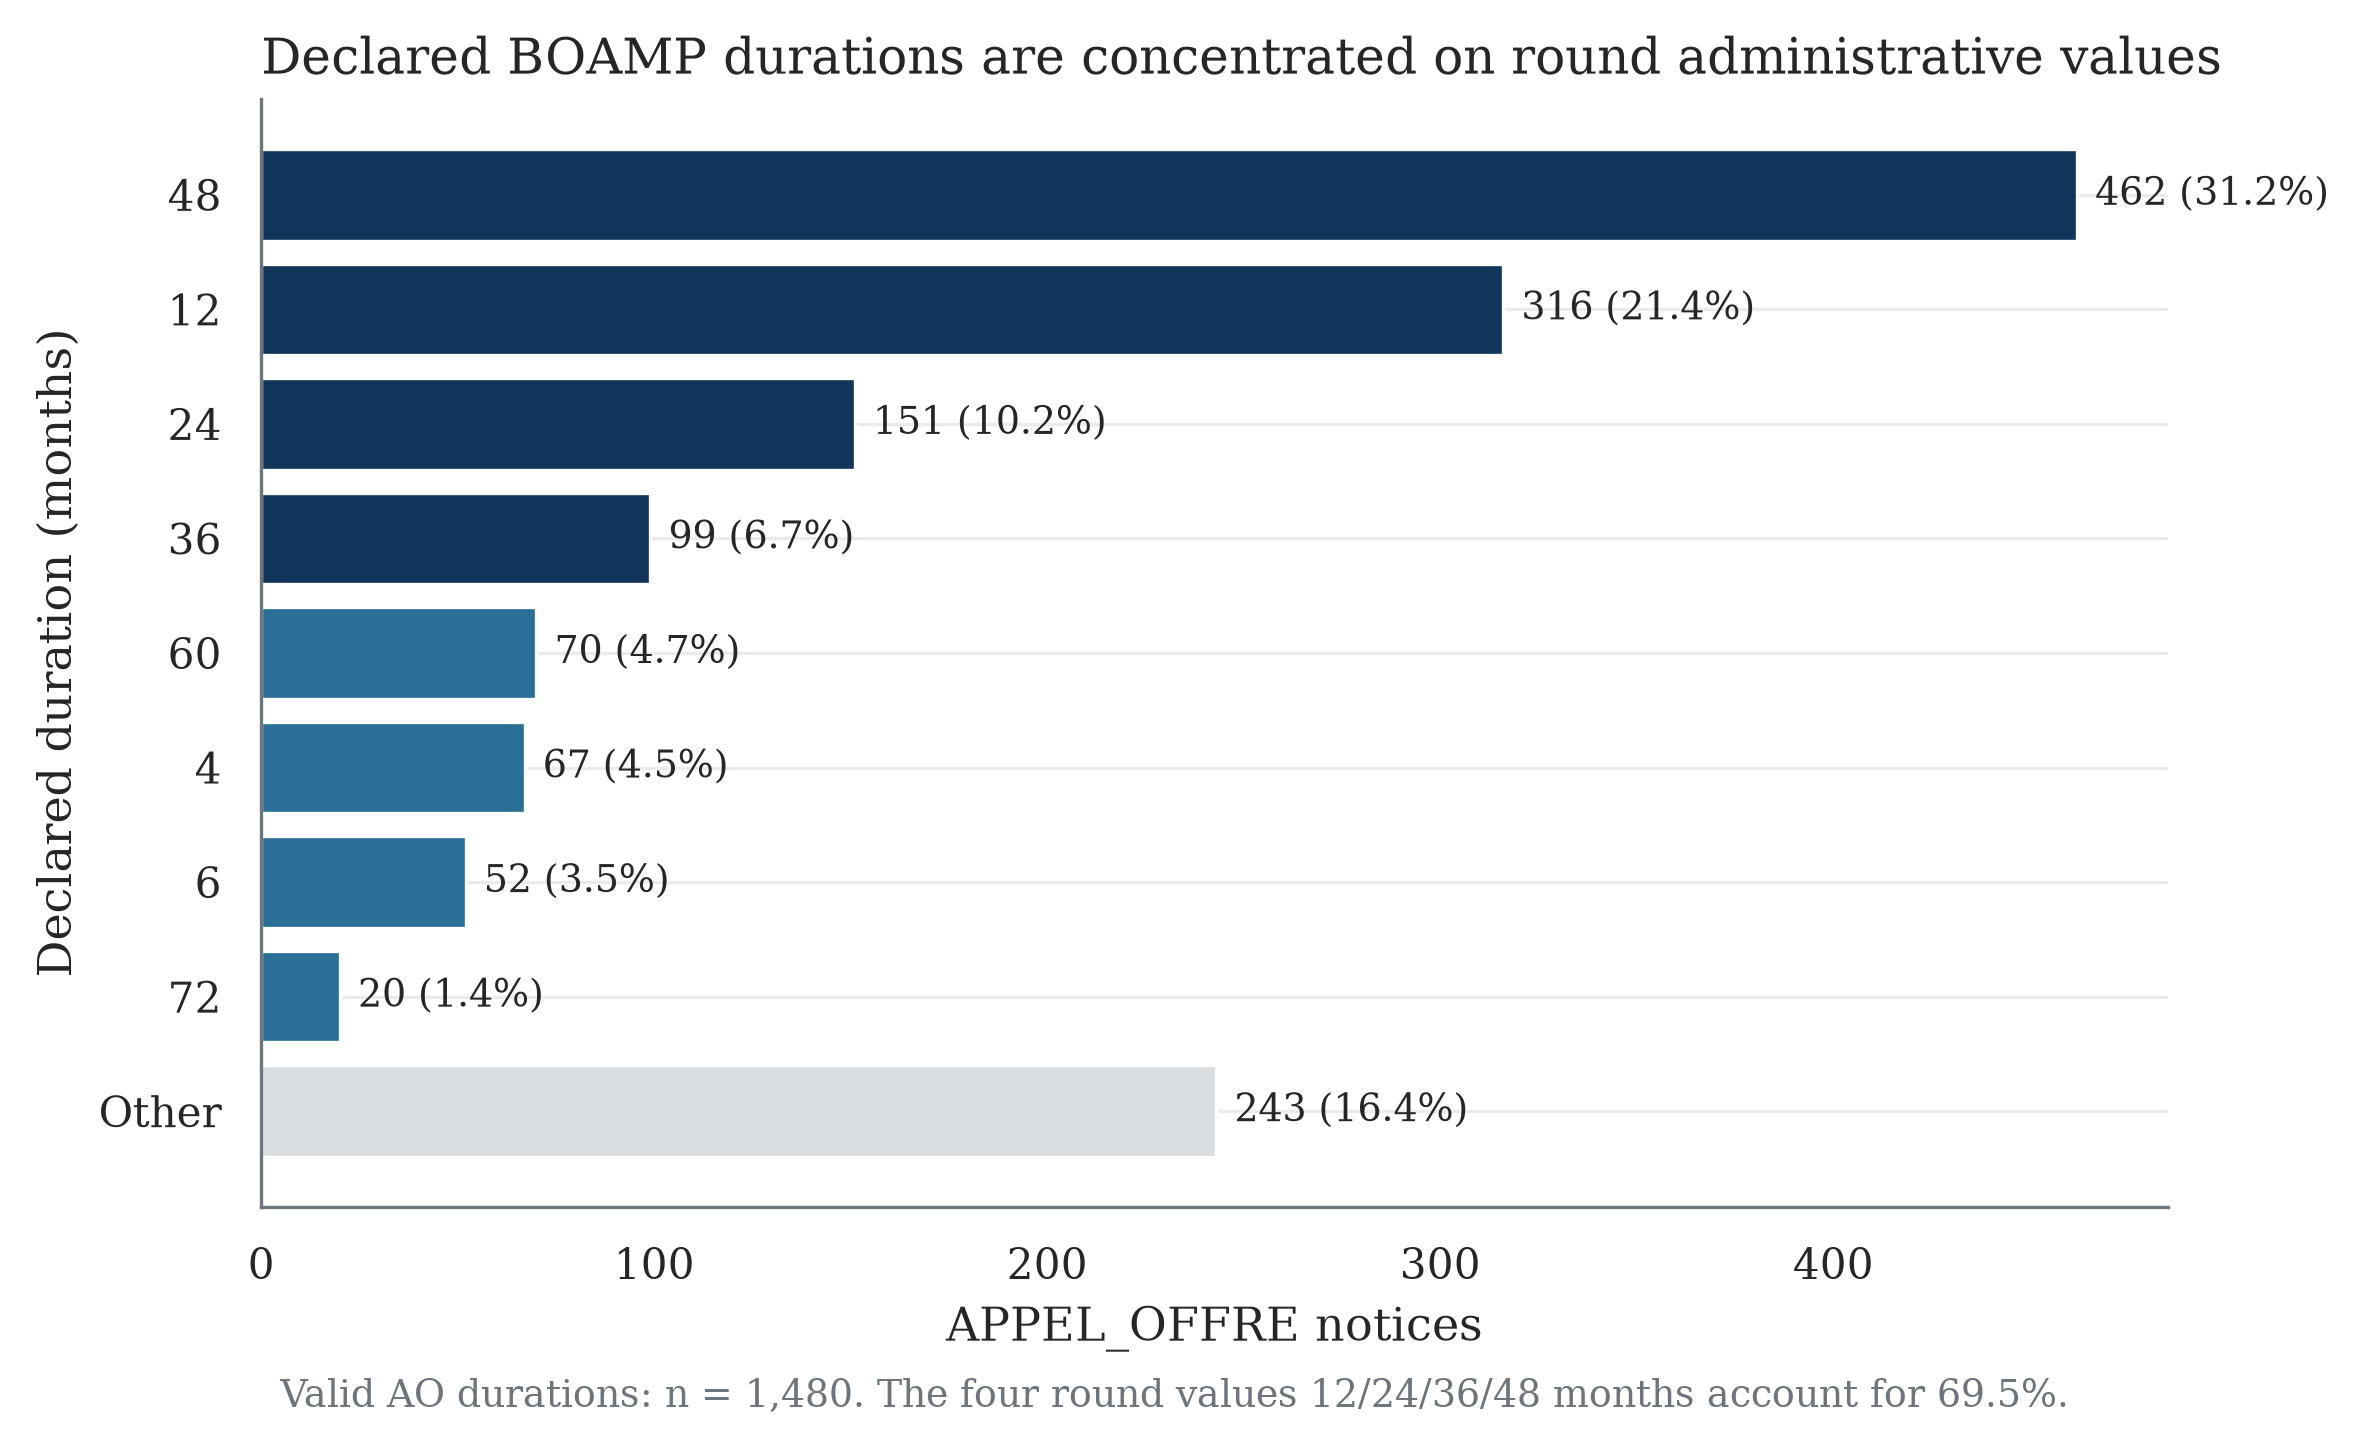
\includegraphics[width=0.90\textwidth]{figures/fig_duration_dist}
\caption{Distribution of declared duration values for the 1,480 \textit{APPEL\_OFFRE}
notices with a valid \texttt{duration\_clean}. Dark bars mark the four exact round
values (12, 24, 36, 48 months) that together account for 69.5\% of all valid
durations. Light-blue bars are other specific values; grey is all remaining values
combined. The concentration at round multiples of 12 reflects the administrative
maximum declaration required by French procurement law, not empirically measured
contract lifetimes.}
\label{fig:duration_dist}
\end{figure}

\subsubsection*{Explanation}

French public procurement law (Code de la commande publique) requires the buyer
to declare the \textbf{administrative maximum duration} of the contract at the
time of publication. This is defined as the base period plus all possible
renewal tranches stacked end-to-end. A buyer writing a 12-month base contract
with three possible 12-month renewal options declares
\texttt{duration\_months = 48}. The 48 months is a legal ceiling approved at
signature, encoding the outer boundary of the contract, not a forecast of when
the buyer intends to re-enter the market.

Using this field as the survival target would mean training the model on
administrative ceilings rather than on observed behaviour. An AO that declares
48 months but renews after 12 months (at the end of the first base period)
would be incorrectly labelled as a 48-month contract. The error is not random
noise: it is systematically biased upward, because buyers default to the
maximum configured option when completing the publication form.

\subsubsection*{Resolution: What the Field Is Used For}

The declared duration $d_i$ is retained for three specific purposes:

\begin{enumerate}
  \item \textbf{Search prior in the linking algorithm.} The estimated end date
        $\hat{e}_i = t_i + d_i$ defines the centre of the temporal candidate
        window (Section~\ref{sec:duration_science} and Step 2 of the algorithm
        in Section~5). The declared duration tells the algorithm
        \textit{where to look} for a renewal notice, not \textit{what the
        answer is}.

  \item \textbf{Covariate in survival models.} The administrative duration
        choice encodes the contractual structure the buyer selected (single-year
        vs.\ multi-year framework). This is predictive of renewal behaviour
        even when the raw value does not equal the actual time-to-renewal.

  \item \textbf{Right-censoring indicator.} Contracts for which
        $\hat{e}_i = t_i + d_i > T_{\max}$ (December 2024) are excluded from
        the eligible denominator: their renewal window is not observable in the
        study period, regardless of algorithm quality.
\end{enumerate}

\noindent The \textbf{actual survival target} is the observed gap:

\begin{equation}
  T_i^{\text{obs}} = \Delta(i, j^*) = t_{j^*} - t_i \quad \text{(months)}
\end{equation}

stored in \texttt{observed\_duration\_months} in \texttt{boamp\_renewal\_links.csv}.
This quantity is available only for the 697 linked contracts (\texttt{event = 1})
and is the correct input duration for the Cox and Kaplan--Meier models in
Phase 2. For right-censored contracts (\texttt{event = 0}), the survival
model requires a censoring time, which is typically taken as the study end
date minus the contract start date.

% =============================================================================
\section{Data Quality Issues Diagnosed}

Nine data quality issues were identified through systematic EDA. Each directly
affects the accuracy or recall of the renewal linking algorithm.

\clearpage
\begin{landscape}
\thispagestyle{empty}
\begin{table}[p]
\centering
\caption{Data quality issues and their impact on the linking algorithm}
\small
\begin{tabularx}{\linewidth}{@{}C{0.7cm}P{4.3cm}X X@{}}
\toprule
\# & Issue & Observation & Impact on linking \\
\midrule
1 & SIRET coverage low
  & Only 5.8\% of \textit{APPEL\_OFFRE} notices have a SIRET-anchored \texttt{buyer\_key}. The SIRET \emph{field} is present on 9.8\% of AO (9.1\% across all 3,181 notices), but $\sim$46\% of those values fail validation and fall back to the name key; 12.8\% of the 475 unique buyer keys are SIRET-anchored. The rest use normalised name as buyer key
  & Variant spellings split buyer groups $\Rightarrow$ structural misses \\[4pt]
2 & Buyer name variants
  & Same buyer appears under multiple spellings after normalisation
  & False negative links where buyers are split \\[4pt]
3 & CPV missing or generic
  & 3.2\% of AO have no CPV; no records use a generic catch-all code
  & CPV score defaults to neutral (0.5) for those pairs \\[4pt]
4 & Contract amount sparse
  & Only 21.4\% of AO report a valid, non-flagged amount
  & Amount cannot be used as a matching signal \\[4pt]
5 & Duration missing
  & 23.4\% of AO have no duration; imputed to 48 months
  & Wrong imputed duration shifts the temporal window \\[4pt]
6 & Duration suspect values
  & Some raw durations $> 120$ months or $= 0$
  & Removed; fall into imputation bucket \\[4pt]
7 & Contract start date imprecise
  & \texttt{date\_attribution} is 0\% on AO records; publication date used as proxy for 59.3\%
  & Up to several weeks of noise in temporal scoring \\[4pt]
8 & Short or generic \textit{objet}
  & 24 notices have \texttt{objet} $<$ 20 characters
  & Semantic embeddings less discriminative for short texts \\[4pt]
9 & \texttt{annonce\_lie} interpretation
  & Present only on ATTRIBUTION notices (82.9\%); refers to same-contract back-link, not a renewal
  & Used as calibration signal, not as a direct renewal label \\[4pt]
\bottomrule
\end{tabularx}
\normalsize
\end{table}
\end{landscape}
\clearpage

% =============================================================================
\section{Preprocessing Pipeline}

\subsection{Buyer Key Construction}

\begin{equation}
  \texttt{buyer\_key}_i =
  \begin{cases}
    \texttt{SIRET:} s_i & \text{if SIRET } s_i \text{ is available} \\
    \texttt{NAME:} \phi(n_i) & \text{otherwise}
  \end{cases}
\end{equation}

where $\phi(\cdot)$ is the name normalisation function: lowercase, strip
accents, remove punctuation, collapse whitespace.

\subsection{Contract Start Date Refinement}

Award date from linked ATTRIBUTION notices is used when available, falling
back to the publication date:

\begin{equation}
  t_i =
  \begin{cases}
    \text{award\_date}(j) & \text{if } \exists\, j \in \text{ATTR} : \texttt{annonce\_lie}(j) = i \\
    \texttt{dateparution}_i & \text{otherwise}
  \end{cases}
\end{equation}

In practice, 40.7\% of eligible AO obtain a more precise start date through
this refinement.

\subsection{Duration Imputation}

\begin{equation}
  d_i =
  \begin{cases}
    \texttt{duration\_clean}_i & \text{if not missing and not suspect} \\
    d_0 = 48 \text{ months}    & \text{otherwise (23.4\% of AO)}
  \end{cases}
\end{equation}

\subsection{Estimated End Date}

\begin{equation}
  \hat{e}_i = t_i + d_i
\end{equation}

\subsection{Text Normalisation}

The \textit{objet} field is normalised for TF-IDF (used in calibration) and
passed raw to Sentence-Transformers:

\begin{enumerate}
  \item Lowercase
  \item Strip Unicode accents (NFD normalisation)
  \item Keep only characters matching \texttt{[a-z0-9 ]}
  \item Collapse multiple spaces
\end{enumerate}

\subsection{Sentence-Transformer Embeddings}

Each normalised \textit{objet} $\mathbf{o}_i$ is encoded into a 384-dimensional
unit-norm vector:

\begin{equation}
  \mathbf{v}_i = \text{ST}\bigl(\mathbf{o}_i\bigr) \in \mathbb{R}^{384},
  \qquad \|\mathbf{v}_i\|_2 = 1
\end{equation}

Model used: \texttt{paraphrase-multilingual-MiniLM-L12-v2}
(multilingual, 384 dimensions, $\sim$120 MB).

\subsection{Cleaning Statistics Summary}
\label{sec:cleaning_stats}

Tables~\ref{tab:amount_cleaning}--\ref{tab:buyer_norm} quantify the impact of the
Week-2 cleaning rules applied to both sources.

\begin{table}[H]
\centering
\caption{Amount cleaning flags and fill rates by source}
\label{tab:amount_cleaning}
\small
\begin{tabular}{@{}l rrrr@{}}
\toprule
Source & Zero ($=0$) & Tiny ($<$\texteuro1\,k) & Ceiling ($\geq$\texteuro10\,M) & \texttt{amount\_clean} fill \\
\midrule
BOAMP ($n=3{,}181$) & 1 & 9 & 53 & 41.1\% \\
DECP  ($n=3{,}039$) & 31 & 20 & 23 & 93.1\% \\
\bottomrule
\end{tabular}
\normalsize
\end{table}

\noindent Flagged values are set to \texttt{NaN} in \texttt{amount\_clean} but the raw field
is preserved. The low BOAMP fill rate reflects the structural gap documented in
Table~\ref{tab:source_comparison}: amount reporting was mandatory only for eForms
notices (2024+). No amount imputation is applied; median-by-segment imputation is deferred
to Phase 3 modelling.

\begin{table}[H]
\centering
\caption{Duration cleaning and fill rates by source}
\label{tab:duration_cleaning}
\small
\begin{tabular}{@{}l rr@{}}
\toprule
Source & Suspect flags (outside [1, 120] months) & \texttt{duration\_clean} fill \\
\midrule
BOAMP ($n=3{,}181$) & 12 & 47.3\% \\
DECP  ($n=3{,}039$) &  6 & 99.2\% \\
\bottomrule
\end{tabular}
\normalsize
\end{table}

\begin{table}[H]
\centering
\caption{Buyer key normalization results}
\label{tab:buyer_norm}
\small
\begin{tabular}{@{}l rrl@{}}
\toprule
Source & Raw unique names & Canonical keys & SIRET-anchored \\
\midrule
BOAMP & 525 & 502 & 156 rows (4.9\%) \\
DECP  & 278 & 294 & 3,039 rows (100.0\%) \\
\bottomrule
\end{tabular}
\normalsize
\end{table}

\noindent The cross-source buyer bridge is saved to \texttt{buyer\_bridge.csv}. Name
normalisation applies lowercase, accent stripping, punctuation removal, and legal-form
suffix removal (e.g.\ \textit{Commune de}, \textit{SARL}).

% =============================================================================
\section{Renewal Linking Algorithm}

\subsection{Notation}

Let $\mathcal{A}$ denote the set of all \textit{APPEL\_OFFRE} notices. Each
notice $i \in \mathcal{A}$ is represented by:

\begin{itemize}[leftmargin=*]
  \item $t_i$: contract start date, defined as the award date when available,
        otherwise the BOAMP publication date;
  \item $d_i$: contract duration in months, after cleaning and imputation;
  \item $\hat{e}_i = t_i + d_i$: estimated contract end date;
  \item $\text{CPV}_i$: main CPV classification code;
  \item $\mathbf{o}_i$: contract description text (\textit{objet});
  \item $b_i$: buyer identifier, using SIRET when available and normalised
        buyer name otherwise.
\end{itemize}

The goal is to construct, for each eligible source notice $i$, an algorithmic
binary outcome $Y_i$ indicating whether a plausible renewal candidate can be found among later
BOAMP calls-for-tender.

\subsection{Step 1 --- Eligibility Filter}

A notice is \textbf{eligible} to be a renewal source if its estimated renewal
date falls within the study period $[T_{\min}, T_{\max}]$:

\begin{equation}
  i \in \mathcal{A}_{\text{elig}}
  \iff
  T_{\min} \leq \hat{e}_i \leq T_{\max}
  \quad
  \bigl(T_{\min} = \text{2015-01-01},\; T_{\max} = \text{2024-12-31}\bigr)
\end{equation}

\begin{table}[h]
\centering
\caption{Eligibility breakdown}
\begin{tabular}{lr}
\toprule
Population & Count \\
\midrule
Total APPEL\_OFFRE              & 1,933 \\
Not eligible: estimated end date after 2024 & 833 \\
\textbf{Eligible} ($\mathcal{A}_{\text{elig}}$) & \textbf{1,100} \\
\bottomrule
\end{tabular}
\end{table}

Contracts with $\hat{e}_i > T_{\max}$ are excluded from the Phase 1 linking
denominator because the renewal opportunity is not sufficiently observable in
the 2015--2024 dataset.

\subsection{Step 2 --- Candidate Pool}

For each eligible source $i$, the candidate pool is:

\begin{equation}
  \mathcal{C}(i) = \bigl\{
    j \in \mathcal{A} :
    b_j = b_i,\quad
    t_j > t_i,\quad
    |t_j - \hat{e}_i| \leq W
  \bigr\},
  \quad W = 12 \text{ months}
\end{equation}

The gap between source and candidate is:

\begin{equation}
  \Delta(i,j) = t_j - t_i \quad \text{(in months)}
\end{equation}

\textbf{Key design choice:} candidates are grouped by \texttt{buyer\_key} only.
The previous baseline grouped by \texttt{[buyer\_key, cpv\_div2]}, which
rejected valid renewals where the buyer reclassified the service under a
different CPV code.

\subsection{Step 3 --- Component Scores}

\paragraph{Text similarity.}
Cosine similarity between unit-norm embeddings (dot product = cosine when
both vectors are $\ell_2$-normalised):

\begin{equation}
  s_{\text{text}}(i,j) = \mathbf{v}_i \cdot \mathbf{v}_j
\end{equation}

\noindent In theory, cosine similarity lies in $[-1,1]$. In this application,
the hard text-similarity filter below retains only candidate pairs with
$s_{\text{text}}(i,j) \geq 0.20$.

\paragraph{CPV compatibility.}
A 4-level step function. A CPV code is treated as generic if it ends in
\texttt{000000}, for example \texttt{72000000} for generic IT services.

\begin{equation}
  s_{\text{cpv}}(i,j) =
  \begin{cases}
    0.5 & \text{either CPV missing} \\
    0.5 & \text{either generic \& same 2-digit div.} \\
    0.0 & \text{either generic \& different div.} \\
    1.0 & \text{CPV}[:4]_i = \text{CPV}[:4]_j \text{ (same class)} \\
    0.7 & \text{CPV}[:2]_i = \text{CPV}[:2]_j \text{ (same division)} \\
    0.3 & \text{CPV}[:1]_i = \text{CPV}[:1]_j \text{ (same section)} \\
    0.0 & \text{otherwise}
  \end{cases}
\end{equation}

\paragraph{Temporal proximity.}
Linear decay from 1.0 at the exact expected renewal date to 0.0 at the
window boundary $W = 12$ months:

\begin{equation}
  s_{\text{temp}}(i,j) = \max\!\left(0,\; 1 - \frac{|\Delta(i,j) - d_i|}{W}\right)
\end{equation}

\paragraph{Buyer match.}
Always 1.0 within the same-buyer grouping loop:

\begin{equation}
  s_{\text{buyer}}(i,j) = 1.0
\end{equation}

\noindent Buyer identity is therefore mainly a \emph{blocking rule}: candidates
are first restricted to the same buyer group. The constant buyer score does not
change the ranking among candidates for the same source contract, but it is kept
explicit to document the full matching design and to allow future extension to
cross-buyer matching.

\subsection{Step 4 --- Composite Score}

\begin{equation}
  \boxed{
    S(i,j) =
    0.40\cdot s_{\text{text}} +
    0.25\cdot s_{\text{cpv}} +
    0.20\cdot s_{\text{temp}} +
    0.15\cdot s_{\text{buyer}}
  }
\end{equation}

\begin{table}[h]
\centering
\caption{Weight rationale}
\begin{tabular}{@{}P{2.5cm}R{1.4cm}P{9.0cm}@{}}
\toprule
Component & Weight & Rationale \\
\midrule
$s_{\text{text}}$   & 0.40 & Strongest discriminator. Semantic similarity captures service identity beyond
                              lexical overlap. Calibration shows ST cosine $\geq$ 0.30 for 96\% of verified
                              same-contract pairs. \\[4pt]
$s_{\text{cpv}}$    & 0.25 & Structured and reliable when specific. Degrades gracefully through 4 levels.
                              Not used as a hard gate because buyers sometimes reclassify. \\[4pt]
$s_{\text{temp}}$   & 0.20 & Rewards timing alignment without hard-excluding distant candidates
                              (hard filters apply separately). \\[4pt]
$s_{\text{buyer}}$  & 0.15 & Constant within the loop; kept explicit so all weights sum to 1.0.
                              Included for future extension to cross-buyer matching. \\
\bottomrule
\end{tabular}
\end{table}

\subsection{Step 5 --- Hard Filters}

Two hard gates are applied before best-match selection:

\begin{align}
  s_{\text{text}}(i,j) &\geq 0.20 \label{eq:f1} \\
  \Delta(i,j) &\in [6,\; 72] \text{ months} \label{eq:f2}
\end{align}

The minimum gap of 6 months prevents matching a contract to itself or to an
immediate amendment. The maximum gap of 72 months (6 years) covers contracts
with the longest expected durations.

\noindent CPV is intentionally \textbf{not} used as a hard filter. Requiring CPV
agreement as a gate would exclude legitimate renewals when the same buyer
reclassifies a similar service under a different CPV code.

Let $\mathcal{F}(i)$ denote the filtered candidate set:

\begin{equation}
  \mathcal{F}(i) =
  \bigl\{
    j \in \mathcal{C}(i) :
    s_{\text{text}}(i,j) \geq 0.20,\;
    \Delta(i,j) \in [6,72]
  \bigr\}.
\end{equation}

\subsection{Step 6 --- Best-Match Selection}

For each source, keep the single highest-scoring candidate:

\begin{equation}
  j^*(i) = \operatorname*{arg\,max}_{j \in \mathcal{F}(i)}\; S(i,j)
\end{equation}

where $\mathcal{F}(i) \subseteq \mathcal{C}(i)$ is the subset passing both
hard filters~(\ref{eq:f1}) and (\ref{eq:f2}).

\subsection{Step 7 --- Outcome Variable}

The Phase 1 binary outcome is an \emph{algorithmic linking outcome}. It records
whether the matching rule found a plausible renewal candidate for source
contract $i$.

\begin{equation}
  Y_i =
	  \begin{cases}
	    1 & \text{if } \mathcal{F}(i) \neq \emptyset \quad \text{(renewal found)} \\
	    0 & \text{if } \mathcal{F}(i) = \emptyset    \quad \text{(no renewal link observed)}
	  \end{cases}
\end{equation}

\noindent The final linking rate is:

\begin{equation}
  \text{Linking rate}
  =
  \frac{\sum_{i \in \mathcal{A}_{\text{elig}}} Y_i}
       {|\mathcal{A}_{\text{elig}}|}
  =
  \frac{697}{1{,}100}
  =
  63.4\%.
\end{equation}

The value $Y_i = 0$ should be interpreted as an unobserved link under the
available data and chosen thresholds, not as definitive evidence that no renewal
occurred.

% =============================================================================
\section{Output Dataset --- Modeling Input}

\subsection{File: \texttt{boamp\_phase2\_survival.csv}}

This is the official BOAMP-only Phase-2 handoff. It is exported from the
notebook linking output and contains one row per eligible
\textit{APPEL\_OFFRE} (1,100 rows, 26 columns).

\small
\begin{longtable}{@{}P{5.0cm}P{1.7cm}P{9.0cm}@{}}
\caption{Column dictionary --- \texttt{boamp\_phase2\_survival.csv} (modeling input)}
\label{tab:links_cols} \\
\toprule
\textbf{Column} & \textbf{Type} & \textbf{Description} \\
\midrule
\endfirsthead
\multicolumn{3}{c}{\tablename\ \thetable{} (continued)} \\
\toprule
\textbf{Column} & \textbf{Type} & \textbf{Description} \\
\midrule
\endhead
\bottomrule
\endlastfoot

\multicolumn{3}{l}{\textit{--- Identifiers ---}} \\[2pt]
\texttt{contract\_id}       & string  & Source contract BOAMP ID (e.g.\ \texttt{BOAMP:15-31464}). \\
\texttt{renewal\_contract\_id} & string & Best-matched renewal contract ID. Empty when \texttt{event=0}. \\[6pt]

\multicolumn{3}{l}{\textit{--- Buyer and classification ---}} \\[2pt]
\texttt{source}            & string  & Constant value \texttt{BOAMP}; makes the handoff schema explicit. \\
\texttt{buyer\_key}         & string  & Buyer identifier (\texttt{SIRET:...} or \texttt{NAME:...}). 308 unique buyers. In practice every row in the final eligible cohort carries a \texttt{NAME:}-based key: no SIRET was populated for any of the 1,100 eligible digital-sector AO contracts, so the \texttt{NAME:} fallback applied universally and name-based grouping governs the entire modeled cohort (and its full candidate pool). This is structural, not incidental: every SIRET-anchored AO is a 2024 eForms notice, and all 2024 contracts are censored upfront (their estimated renewal window falls after the 2024-12-31 study end), so SIRET coverage in the eligible cohort is necessarily zero. SIRET enrichment can therefore only help future (post-2024) data, not the historical survival window. \\
\texttt{cpv\_div2}          & float   & 2-digit CPV division of the source contract. 95.3\% coverage. \\
\texttt{category\_label}    & string  & Internal category (11 levels; see Table~\ref{tab:categories}). \\[6pt]

\multicolumn{3}{l}{\textit{--- Temporal variables ---}} \\[2pt]
\texttt{start\_date}        & date    & Source contract start date (refined from award date where available). \\
\texttt{declared\_duration\_months} & float & Contract duration as declared (or imputed). Mean: 31.5 months. \\
\texttt{dur\_was\_imputed}  & bool    & True if duration was set to the default 48-month imputation (25.1\% of rows). \\
\texttt{estimated\_end\_date} & date  & $\hat{e}_i = t_i + d_i$; defines the renewal search window. \\
\texttt{observed\_duration\_months} & float & Survival time in months, always filled. For \texttt{event=1}: actual renewal gap $\Delta(i,j^*)$. For \texttt{event=0}: right-censoring duration from contract start to end of study period. \\
\texttt{renewal\_duration\_months} & float & Observed renewal gap for linked contracts only. Filled on 63.4\% of rows (the \texttt{event=1} subset). \\
\texttt{censoring\_duration\_months} & float & Observed time-to-study-end for censored contracts only. Filled on 36.6\% of rows (the \texttt{event=0} subset). \\[6pt]

\multicolumn{3}{l}{\textit{--- Outcome variable ---}} \\[2pt]
\texttt{event}              & int     & \textbf{Target variable}. 1 = plausible renewal link found (697), 0 = no renewal link observed under the algorithm (403). \\[6pt]

\multicolumn{3}{l}{\textit{--- Matching scores (linked rows only) ---}} \\[2pt]
\texttt{composite\_score}   & float   & $S(i,j^*)$. Mean: 0.624, range: 0.251--0.998. \\
\texttt{text\_similarity}   & float   & $s_{\text{text}}(i,j^*)$. Mean: 0.513, range: 0.200--1.000. \\
\texttt{cpv\_match\_score}  & float   & $s_{\text{cpv}}(i,j^*)$. Mean: 0.527, range: 0.000--1.000. \\
\texttt{temporal\_score}    & float   & $s_{\text{temp}}(i,j^*)$. Mean: 0.684, range: 0.007--1.000. \\[6pt]

\multicolumn{3}{l}{\textit{--- Metadata ---}} \\[2pt]
\texttt{start\_date\_source} & string & How $t_i$ was obtained: \texttt{publication\_date} (59.3\%) or \texttt{attribution\_award\_date} (40.7\%). \\
\texttt{link\_method}       & string  & Algorithm used: \texttt{sentence\_transformers} (697 rows) or \texttt{none} (403 rows). \\[6pt]

\multicolumn{3}{l}{\textit{--- Covariates (joined from \texttt{boamp\_full\_clean.csv}) ---}} \\[2pt]
\texttt{amount\_clean}      & float   & Contract amount (EUR) after quality filtering; NaN when any amount flag is True. Fill rate: 20.3\% (BOAMP-only limitation). \\
\texttt{flag\_amount\_zero} & bool    & True if raw amount = 0 (encoding artefact). \\
\texttt{flag\_amount\_tiny} & bool    & True if raw amount $\in$ (0, 1\,000) EUR (implausible for an IT contract). \\
\texttt{flag\_amount\_ceiling} & bool & True if raw amount $\geq$ 10\,000\,000 EUR (likely framework-agreement ceiling). \\
\texttt{type\_procedure}    & string  & Procurement procedure type (e.g.\ \textit{Proc\'edure adapt\'ee}, \textit{Appel d'offres ouvert}). Fill rate: 99.7\%. \\
\texttt{type\_marche}       & string  & Contract type (e.g.\ \textit{March\'e}, \textit{Accord-cadre}). Fill rate: 85.6\%. \\
\end{longtable}
\normalsize

\subsection{Score Distributions for Linked Contracts}

Table~\ref{tab:score_dist} reports the distribution of matching scores among
the 697 linked contracts. These statistics are useful diagnostics, but they
should not be interpreted as independent validation: the same scores are used
by the algorithm to select the links. The low minimum values, especially for
the composite, CPV, and temporal scores, indicate that some accepted links are
low-confidence cases that should be checked in the Phase 2 validation sample.

\begin{table}[H]
\centering
\caption{Descriptive statistics of matching scores (event=1 rows only, n=697)}
\label{tab:score_dist}
\begin{tabular}{lrrrrrrr}
\toprule
Score & Mean & Std & Min & Q25 & Median & Q75 & Max \\
\midrule
\texttt{composite\_score}  & 0.624 & 0.143 & 0.251 & 0.520 & 0.622 & 0.716 & 0.998 \\
\texttt{text\_similarity}  & 0.513 & 0.202 & 0.200 & 0.360 & 0.475 & 0.619 & 1.000 \\
\texttt{cpv\_match\_score} & 0.527 & 0.353 & 0.000 & 0.300 & 0.500 & 0.700 & 1.000 \\
\texttt{temporal\_score}   & 0.684 & 0.255 & 0.007 & 0.541 & 0.758 & 0.896 & 1.000 \\
\bottomrule
\end{tabular}
\end{table}

\begin{figure}[H]
\centering
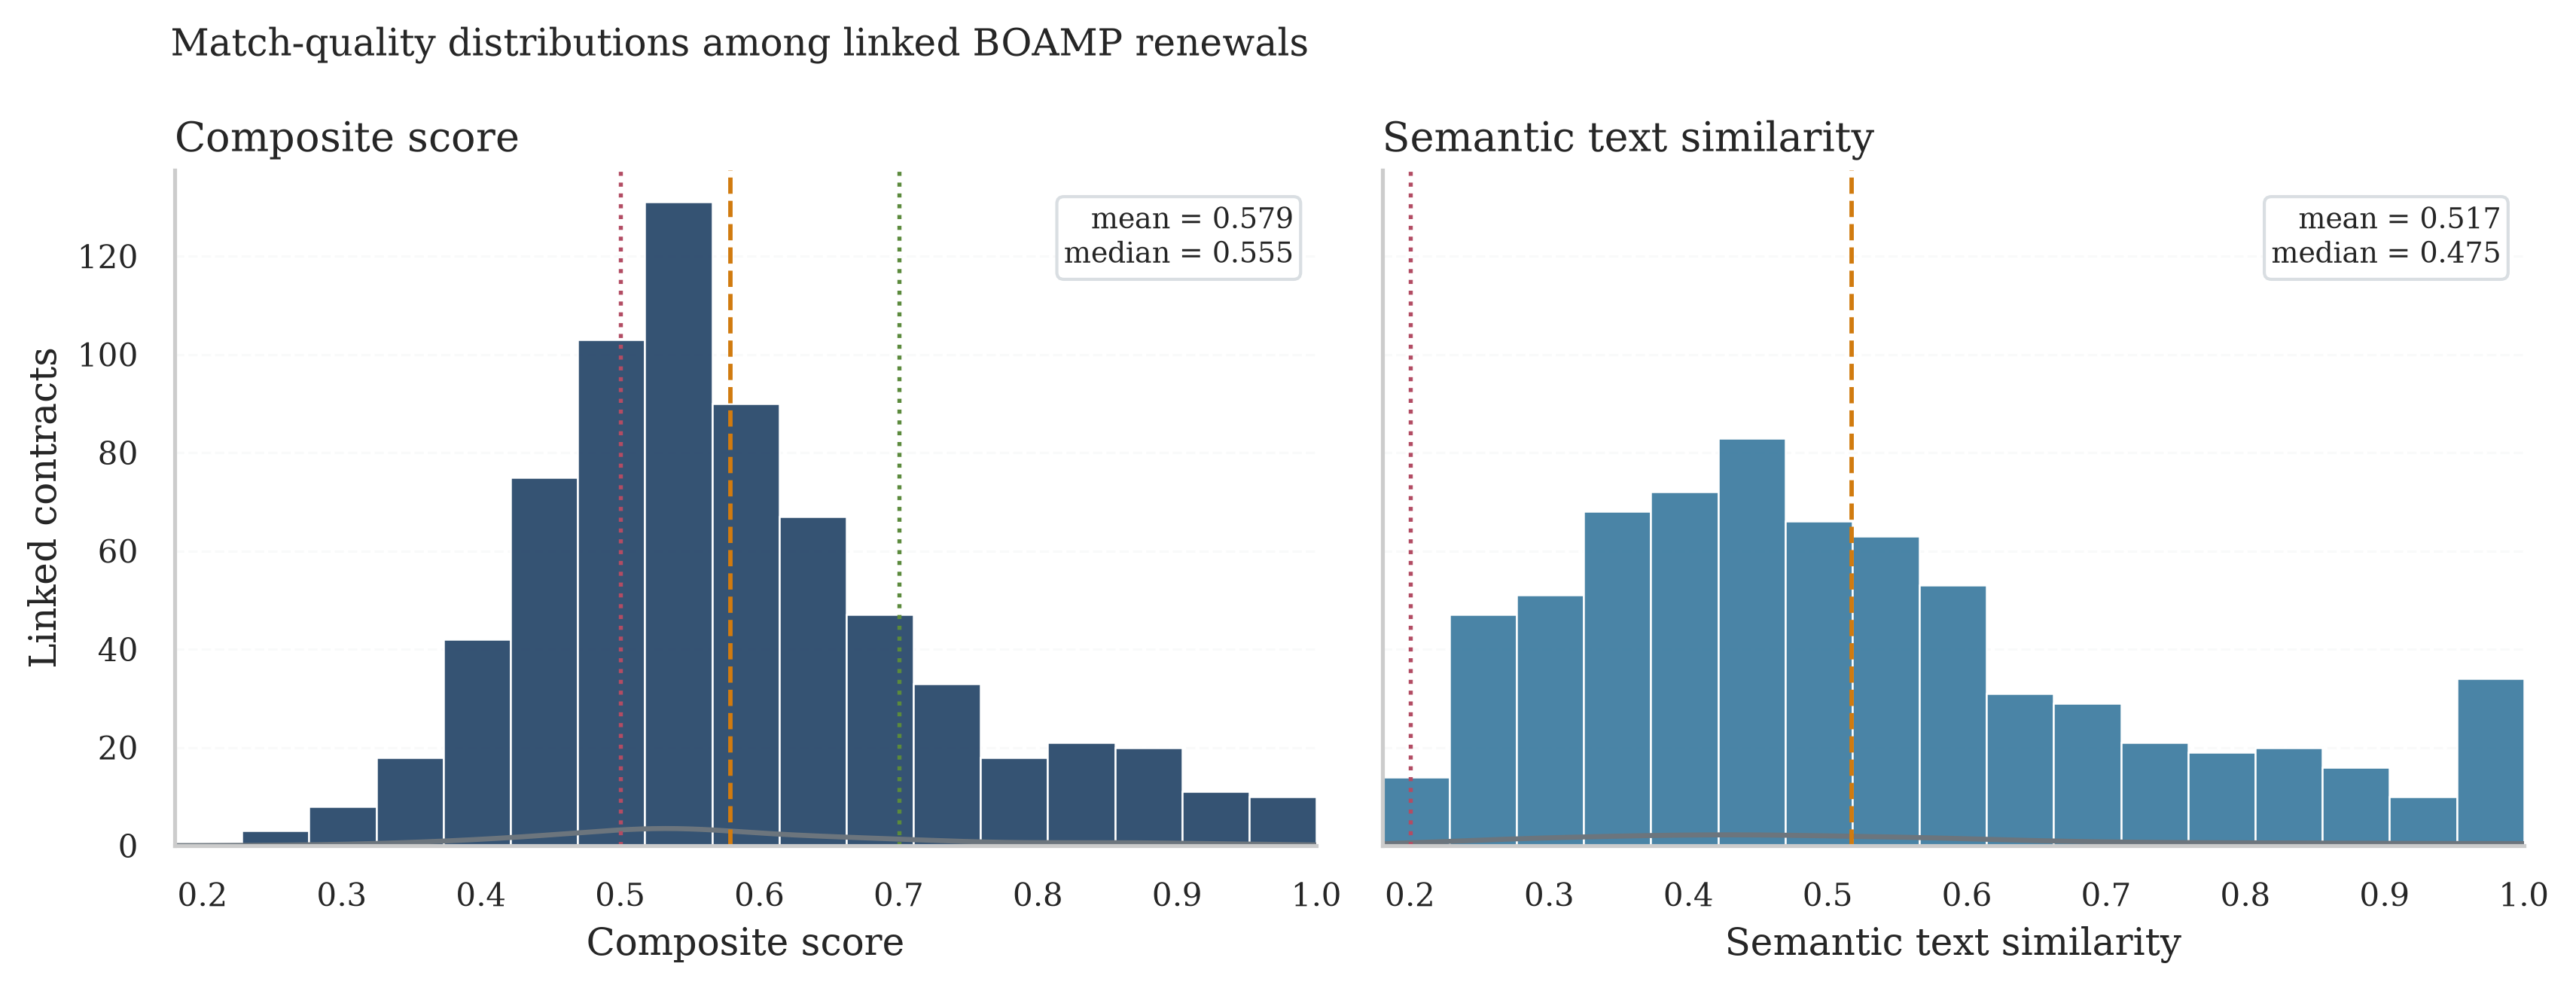
\includegraphics[width=0.96\textwidth]{figures/fig_score_distributions}
\caption{Score distributions for the 697 linked contracts (\texttt{event = 1}).
\textbf{Left:} composite score $S(i,j^*)$ with confidence-tier shading: LOW
(composite $< 0.50$, red, $n = 144$), MEDIUM ($0.50$--$0.70$, orange, $n = 348$),
HIGH ($\geq 0.70$, green, $n = 205$). The dashed line marks the mean (0.624).
\textbf{Right:} text similarity $s_{\text{text}}(i,j^*)$ with the hard-filter
threshold at 0.20 (dotted red). The shaded band (0.20--0.30) flags 89 pairs
(12.8\%) whose semantic similarity is low, representing the highest false-positive
risk.}
\label{fig:score_dist}
\end{figure}

\subsection{Declared vs.\ Observed Duration}

Table~\ref{tab:duration_stats} compares the declared contract duration with the
gap between the source notice and the selected renewal candidate. This is a
consistency check for the temporal matching logic, not external proof that the
selected pairs are true renewals, because declared duration is already used to
define the candidate window and the temporal score.

\begin{table}[H]
\centering
\caption{Duration statistics (months)}
\label{tab:duration_stats}
\begin{tabular}{lrrrrrrr}
\toprule
 & Mean & Std & Min & Q25 & Median & Q75 & Max \\
\midrule
\texttt{declared\_duration\_months} (all 1,100) & 31.5 & 17.7 & 1 & 12 & 36 & 48 & 72 \\
\texttt{observed\_duration\_months} (697 linked) & 32.3 & 17.0 & 6 & 13 & 37 & 48 & 71 \\
\bottomrule
\end{tabular}
\end{table}

The close medians, 36 months for declared duration and 37 months for the linked
candidate gap, are therefore reassuring but partly mechanical. A stronger
validation should examine the error
$\texttt{observed\_duration\_months} - \texttt{declared\_duration\_months}$,
separately for imputed and non-imputed durations, and combine this with manual
review of a stratified sample of linked pairs.

\begin{figure}[H]
\centering
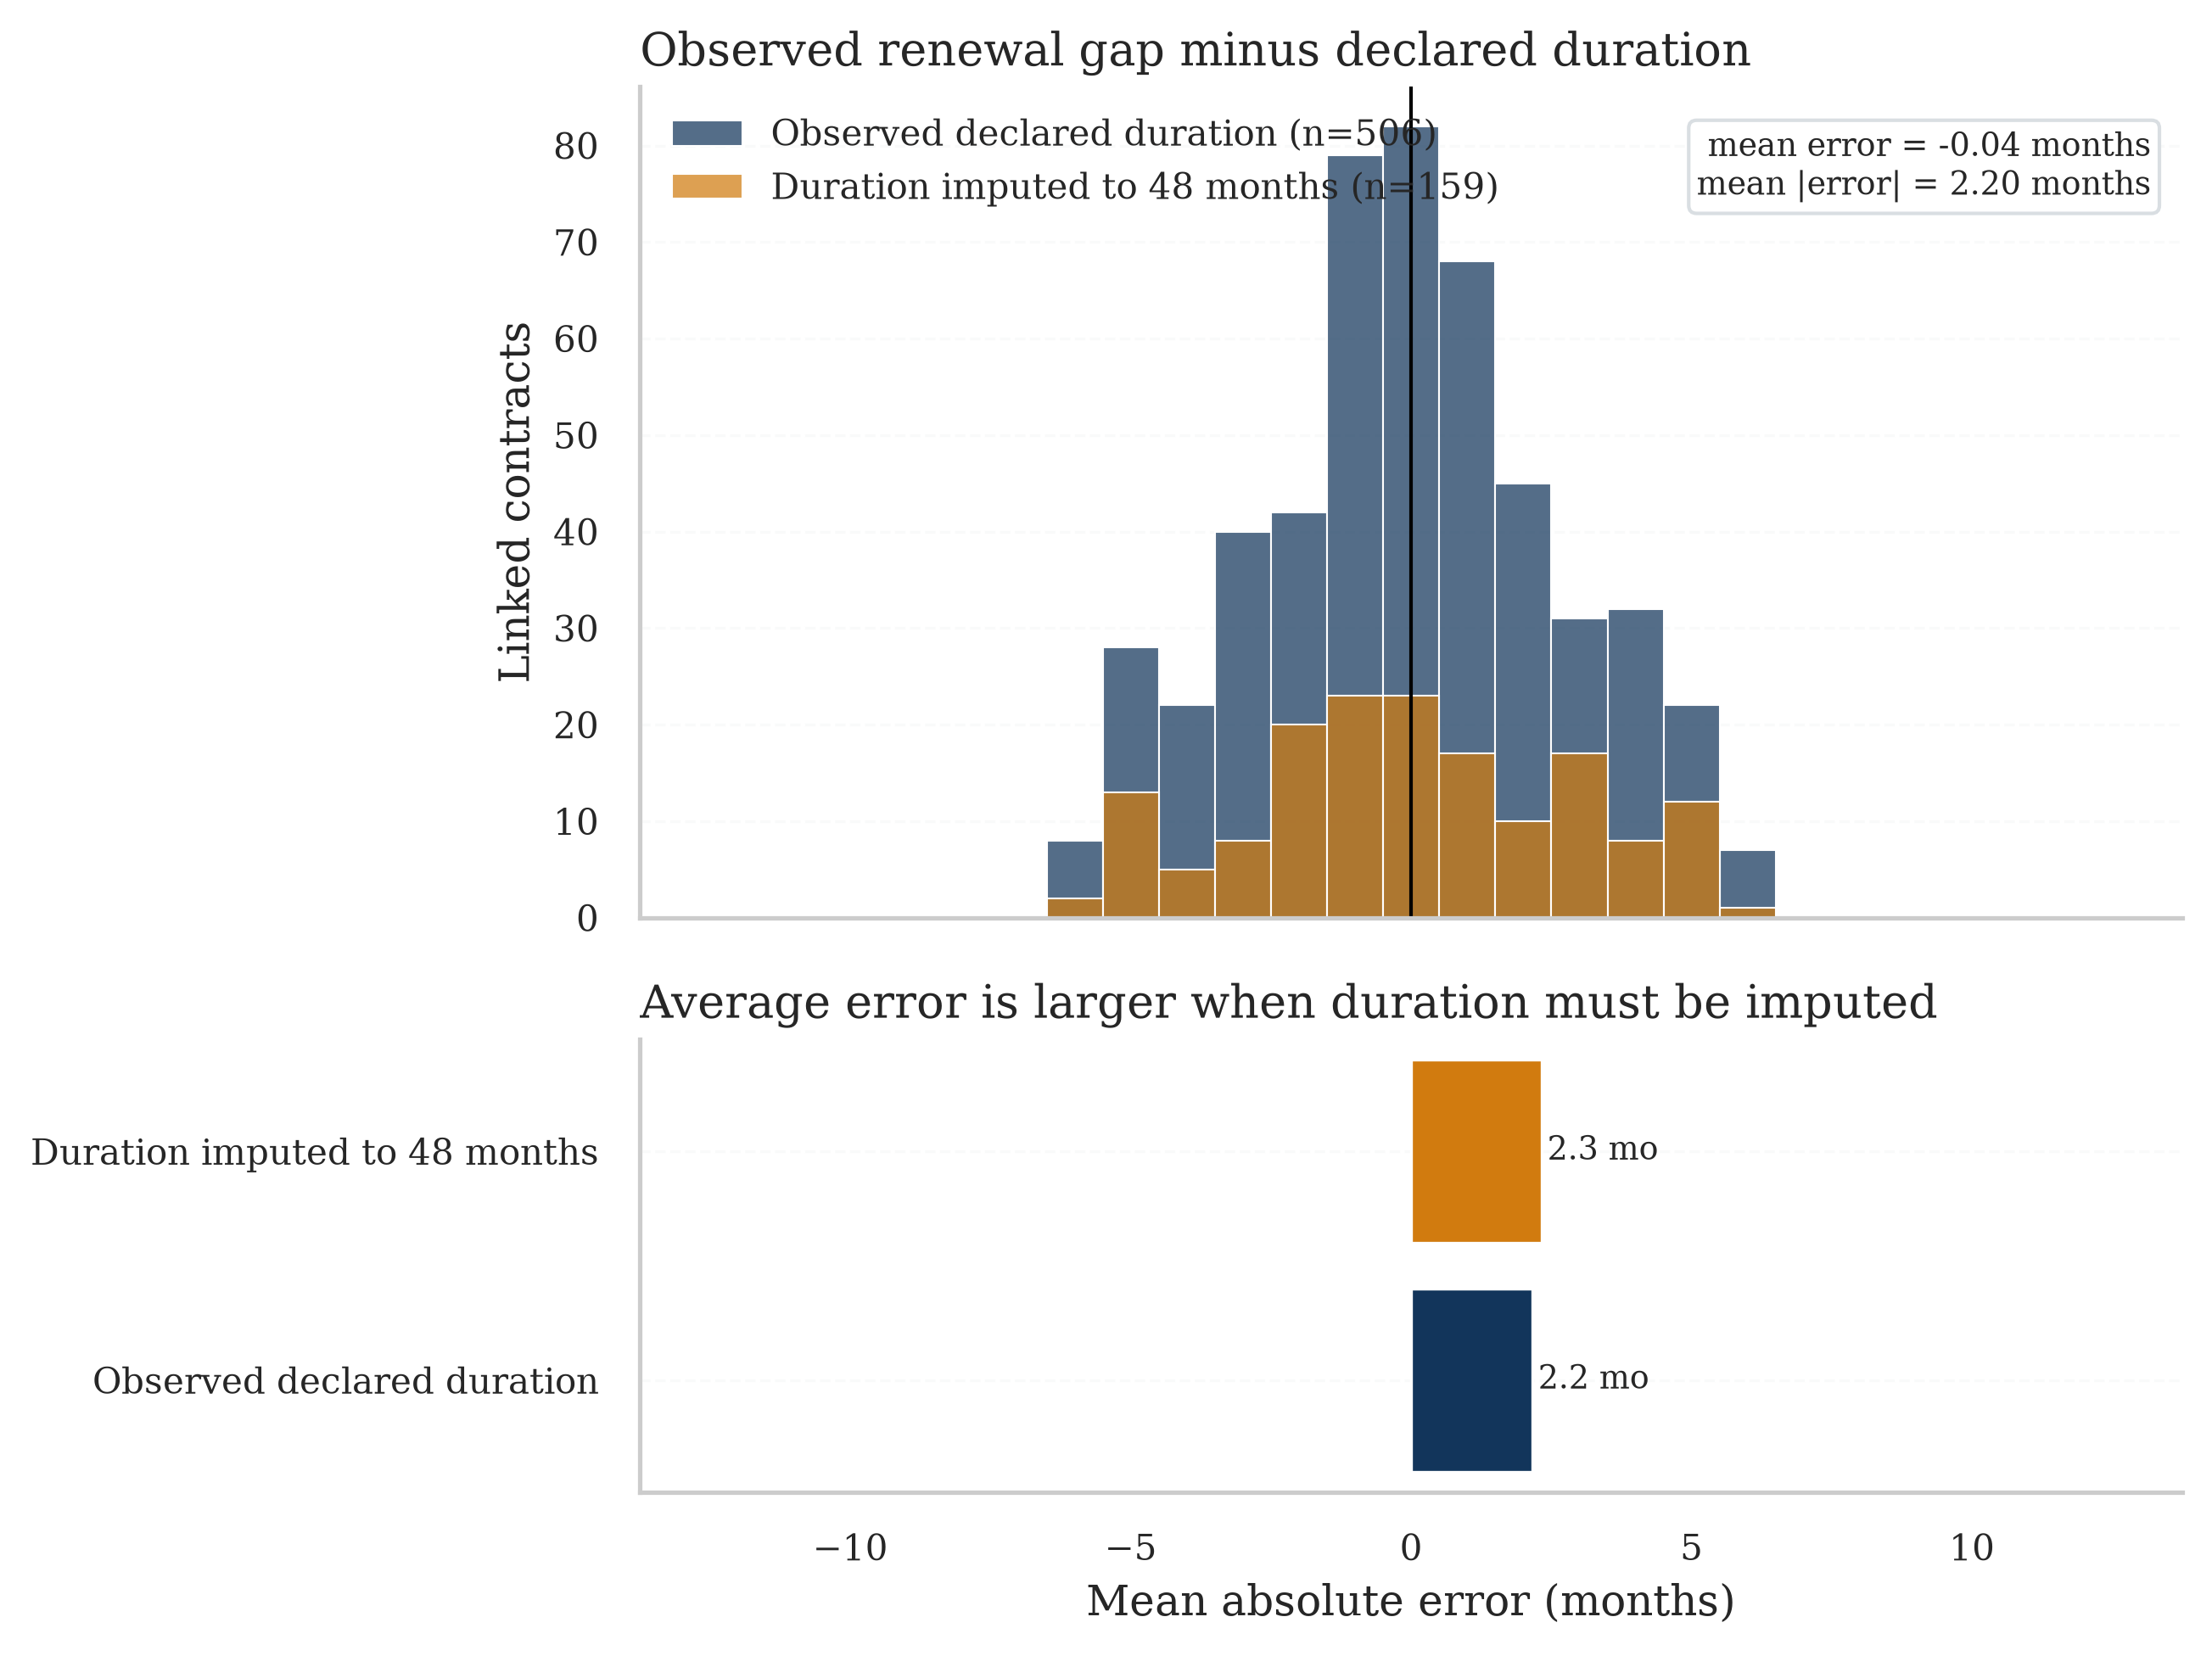
\includegraphics[width=0.82\textwidth]{figures/fig_temporal_error}
\caption{Distribution of the temporal error $\Delta(i,j^*) - d_i$ (observed gap
minus declared duration) for the 697 linked contracts. Blue bars correspond to
the 527 contracts with a valid non-imputed duration; orange bars to the 170
contracts whose duration was imputed to 48 months. The overall mean error is
$-0.04$ months (effectively zero bias) with a standard deviation of 4.87 months.
All pairs fall within $\pm 12$ months by construction of the hard filter, but
the near-zero mean confirms there is no systematic temporal shift in the matches.
Imputed-duration contracts show slightly larger spread (mean $|$error$| = 4.1$
vs.\ $3.7$ months for non-imputed).}
\label{fig:temporal_error}
\end{figure}

% =============================================================================
\section{Results}

\subsection{Linking Rate Comparison}

\begin{table}[h]
\centering
\caption{Linking rate by method}
\begin{tabular}{@{}P{8.7cm}R{1.6cm}R{2.2cm}R{1.5cm}@{}}
\toprule
Method & Linked & Denominator & Rate \\
\midrule
Baseline (Jaccard + buyer $\times$ CPV groupby) & 219 & 1,933 & 11.3\% \\
TF-IDF cosine (intermediate)                    & 279 & 1,100 & 25.4\% \\
\textbf{Sentence-Transformers (final)}          & \textbf{697} & \textbf{1,100} & \textbf{63.4\%} \\
\bottomrule
\end{tabular}
\end{table}

The two key changes responsible for the improvement are:

\begin{enumerate}
  \item \textbf{Grouping by buyer only} (removing CPV as a hard gate): recovers
        contracts where the buyer reclassified the service. The final method
        also reports performance on the 1,100 contracts whose expected renewal
        date is observable within the study period, instead of using all 1,933
        AO notices as the denominator.
  \item \textbf{Sentence-Transformers over TF-IDF}: semantic similarity captures
        meaning beyond lexical overlap, contributing approximately +38 percentage
        points in linking rate compared to TF-IDF alone.
\end{enumerate}

\subsection{Failure Analysis}

Of the 403 unlinked eligible AO, three failure modes are identified:

\begin{table}[h]
\centering
\caption{Failure mode breakdown (403 unlinked eligible AO)}
\small
\begin{tabular}{@{}P{4.4cm}R{1.2cm}R{1.4cm}P{7.5cm}@{}}
\toprule
Failure reason & Count & Share & Description \\
\midrule
\texttt{NO\_TEMPORAL\_PARTNER} & 339 & 84.1\% & No other AO from the same buyer fell in the $\pm$12-month window. Likely structural (buyer issued only one contract in the period). \\[4pt]
\texttt{TEXT\_MISMATCH}        &  40 &  9.9\% & Temporal candidates existed but all had $s_{\text{text}} < 0.20$. Text was too dissimilar even at the semantic level. \\[4pt]
\texttt{CPV\_MISMATCH}         &  24 &  6.0\% & Temporal candidates existed, but the closest diagnostic candidate was in an incompatible CPV section. This label is a diagnostic warning, not a separate CPV hard gate in the final scoring rule. \\
\midrule
\textbf{Total unlinked}        & \textbf{403} & 100\% & \\
\bottomrule
\end{tabular}
\normalsize
\end{table}

The dominant failure mode (\texttt{NO\_TEMPORAL\_PARTNER}, 84.1\%) reflects a
structural ceiling: buyers who published only one call-for-tender within the
study period cannot be linked regardless of algorithm quality. This is the main
remaining ceiling on the 36.6\% unlinked fraction.

\subsection{Linking Rate by Contract Start Year}

Figure~\ref{fig:linking_by_year} disaggregates the linking rate by year of
contract start. Rates are stable between 55\% and 75\% for contracts from
2015 to 2022. The sharp drop to 33\% in 2023 ($n = 12$) is expected: a
contract starting in late 2023 has its estimated renewal window in 2025 or
beyond, outside the study period, so most of these contracts are structurally
right-censored and cannot be linked regardless of algorithm quality.

\begin{figure}[H]
\centering
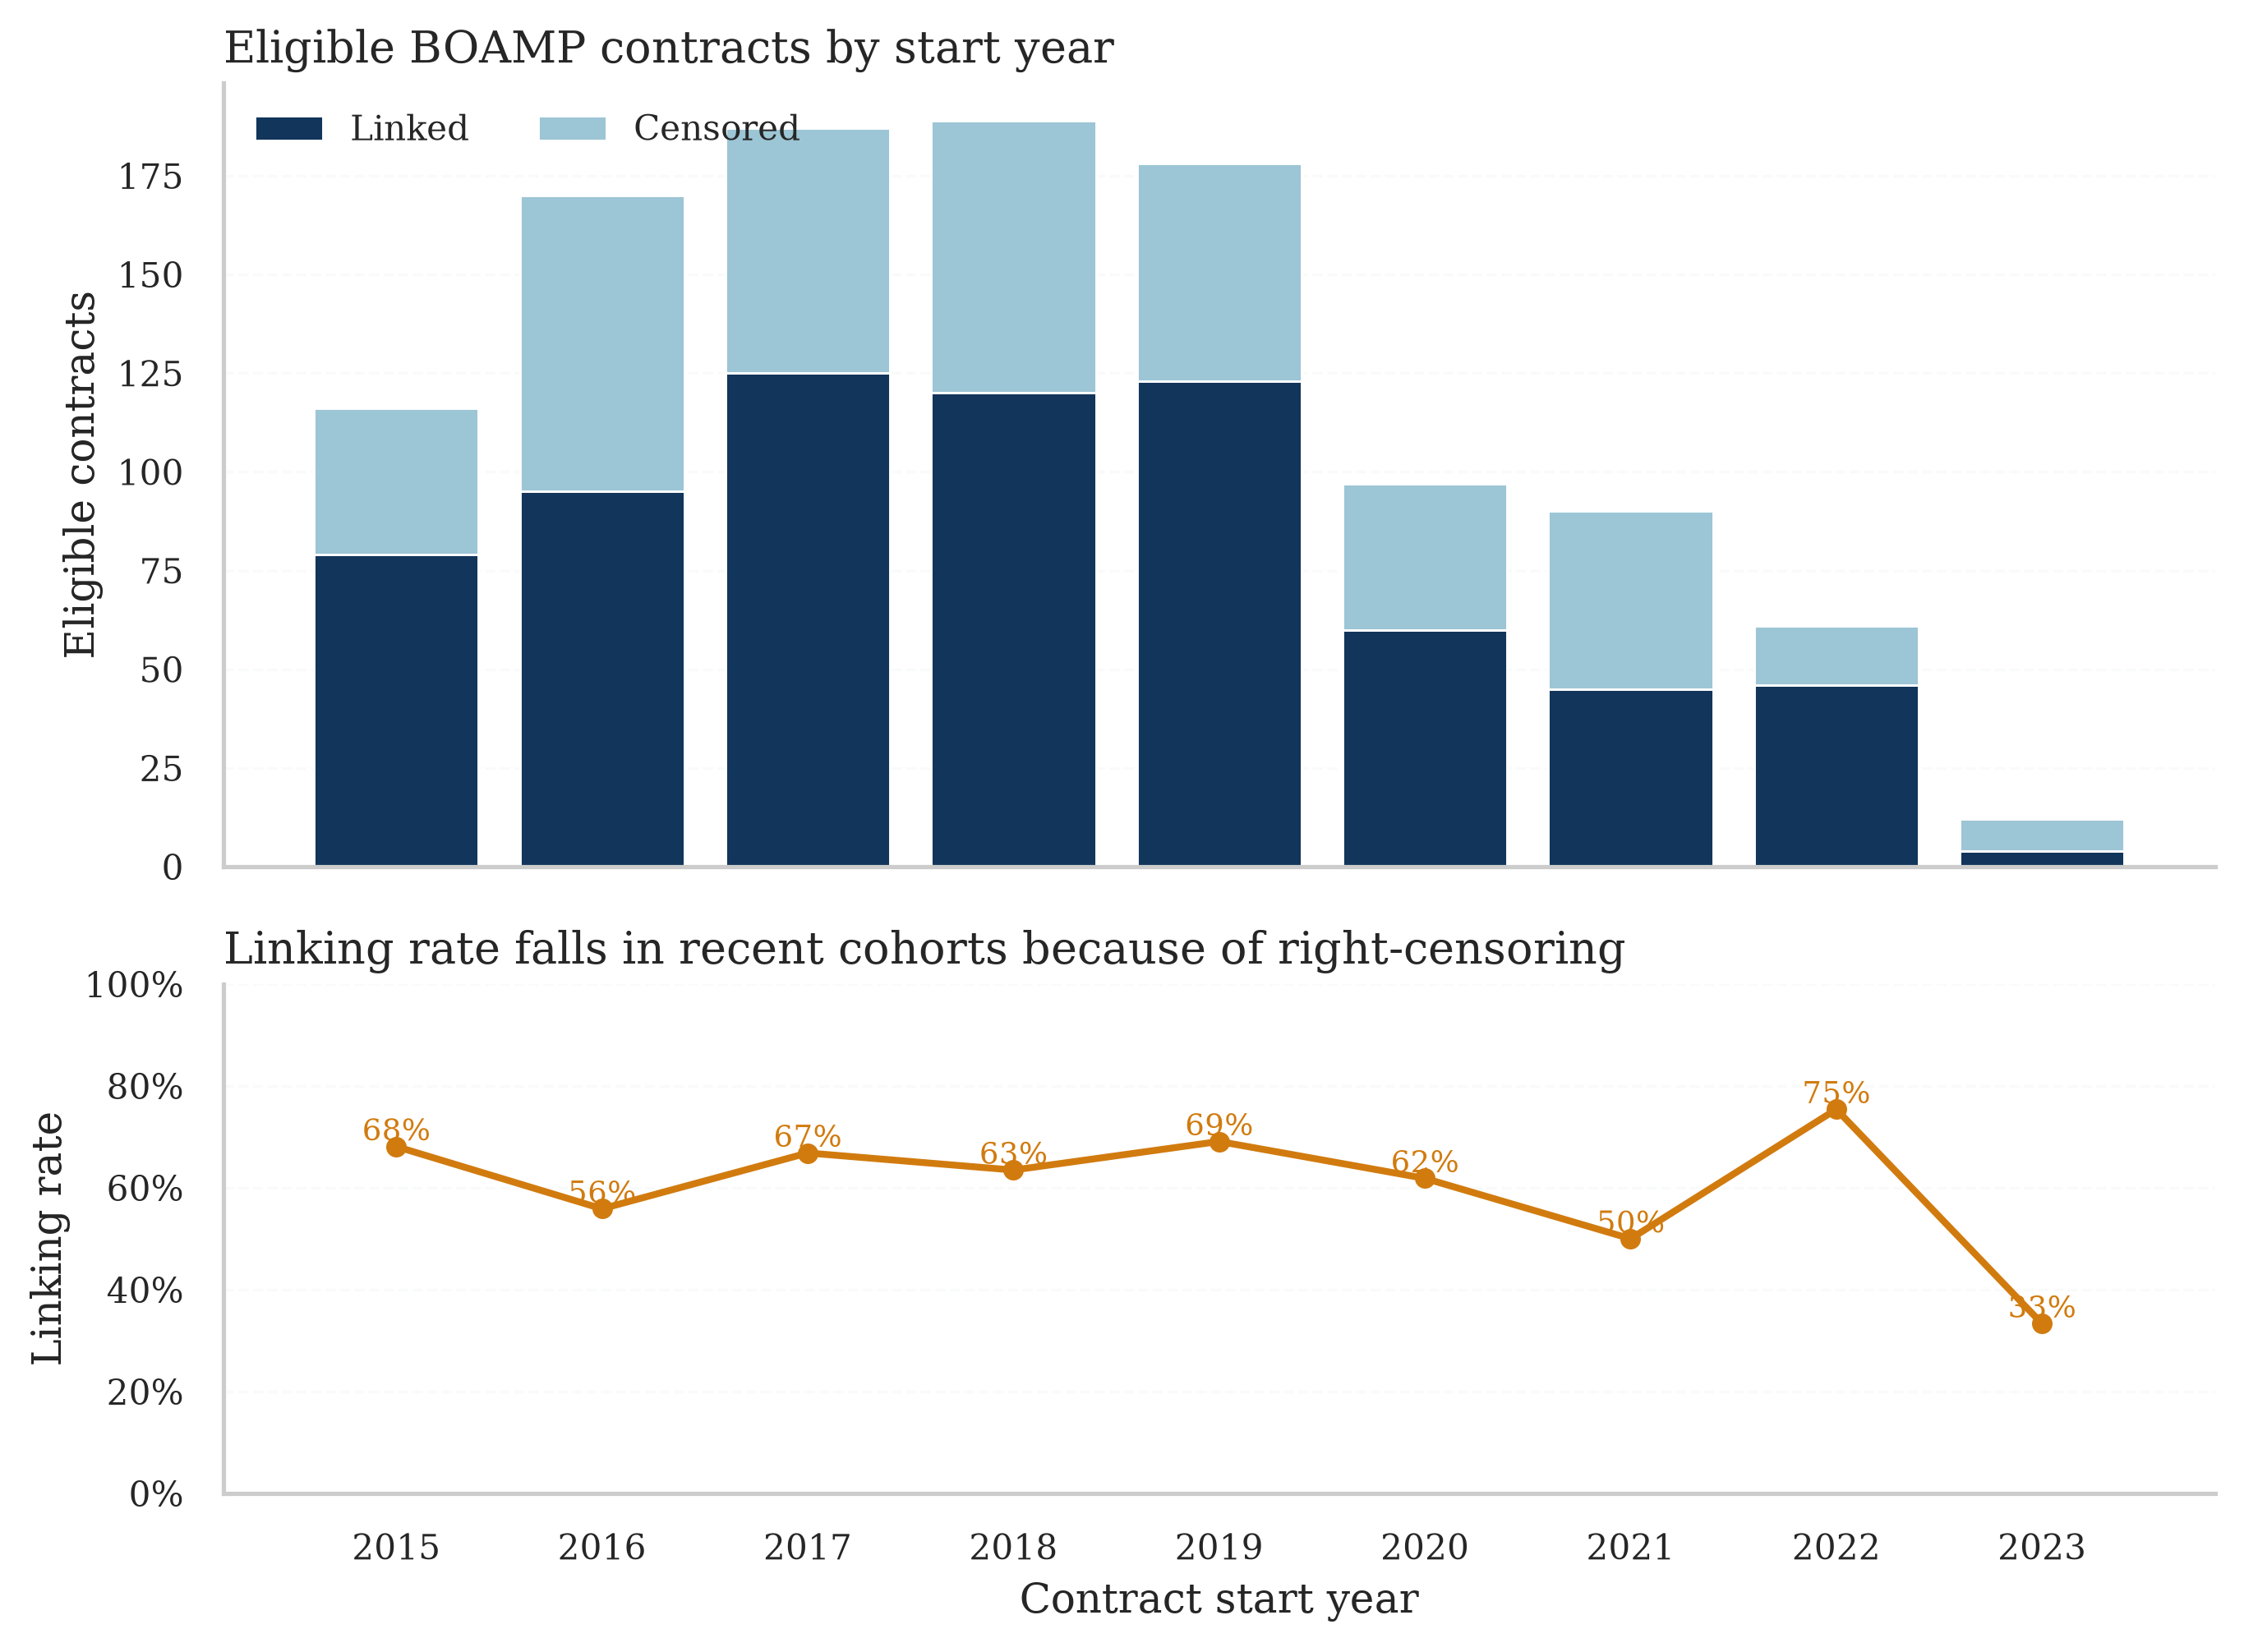
\includegraphics[width=0.92\textwidth]{figures/fig_linking_by_year}
\caption{Linked (dark blue) and unlinked (light blue) eligible contracts by
year of contract start, with the linking rate overlaid as an orange line
(right axis). Rates for 2015--2022 are stable in the range 50--75\%.
The 2023 cohort ($n = 12$) has a 33\% rate due to structural right-censoring:
most contracts starting in late 2023 have their expected renewal window after
December 2024 and cannot be linked in the current study period.}
\label{fig:linking_by_year}
\end{figure}

\subsection{Threshold Sensitivity Analysis}

The linking rate depends on the minimum text-similarity threshold applied as
a hard filter. Figure~\ref{fig:threshold_sensitivity} shows how the number of
retained events and the overall eligible linking rate change as the threshold
is raised from the current value of 0.20 to 0.50.

\begin{figure}[H]
\centering
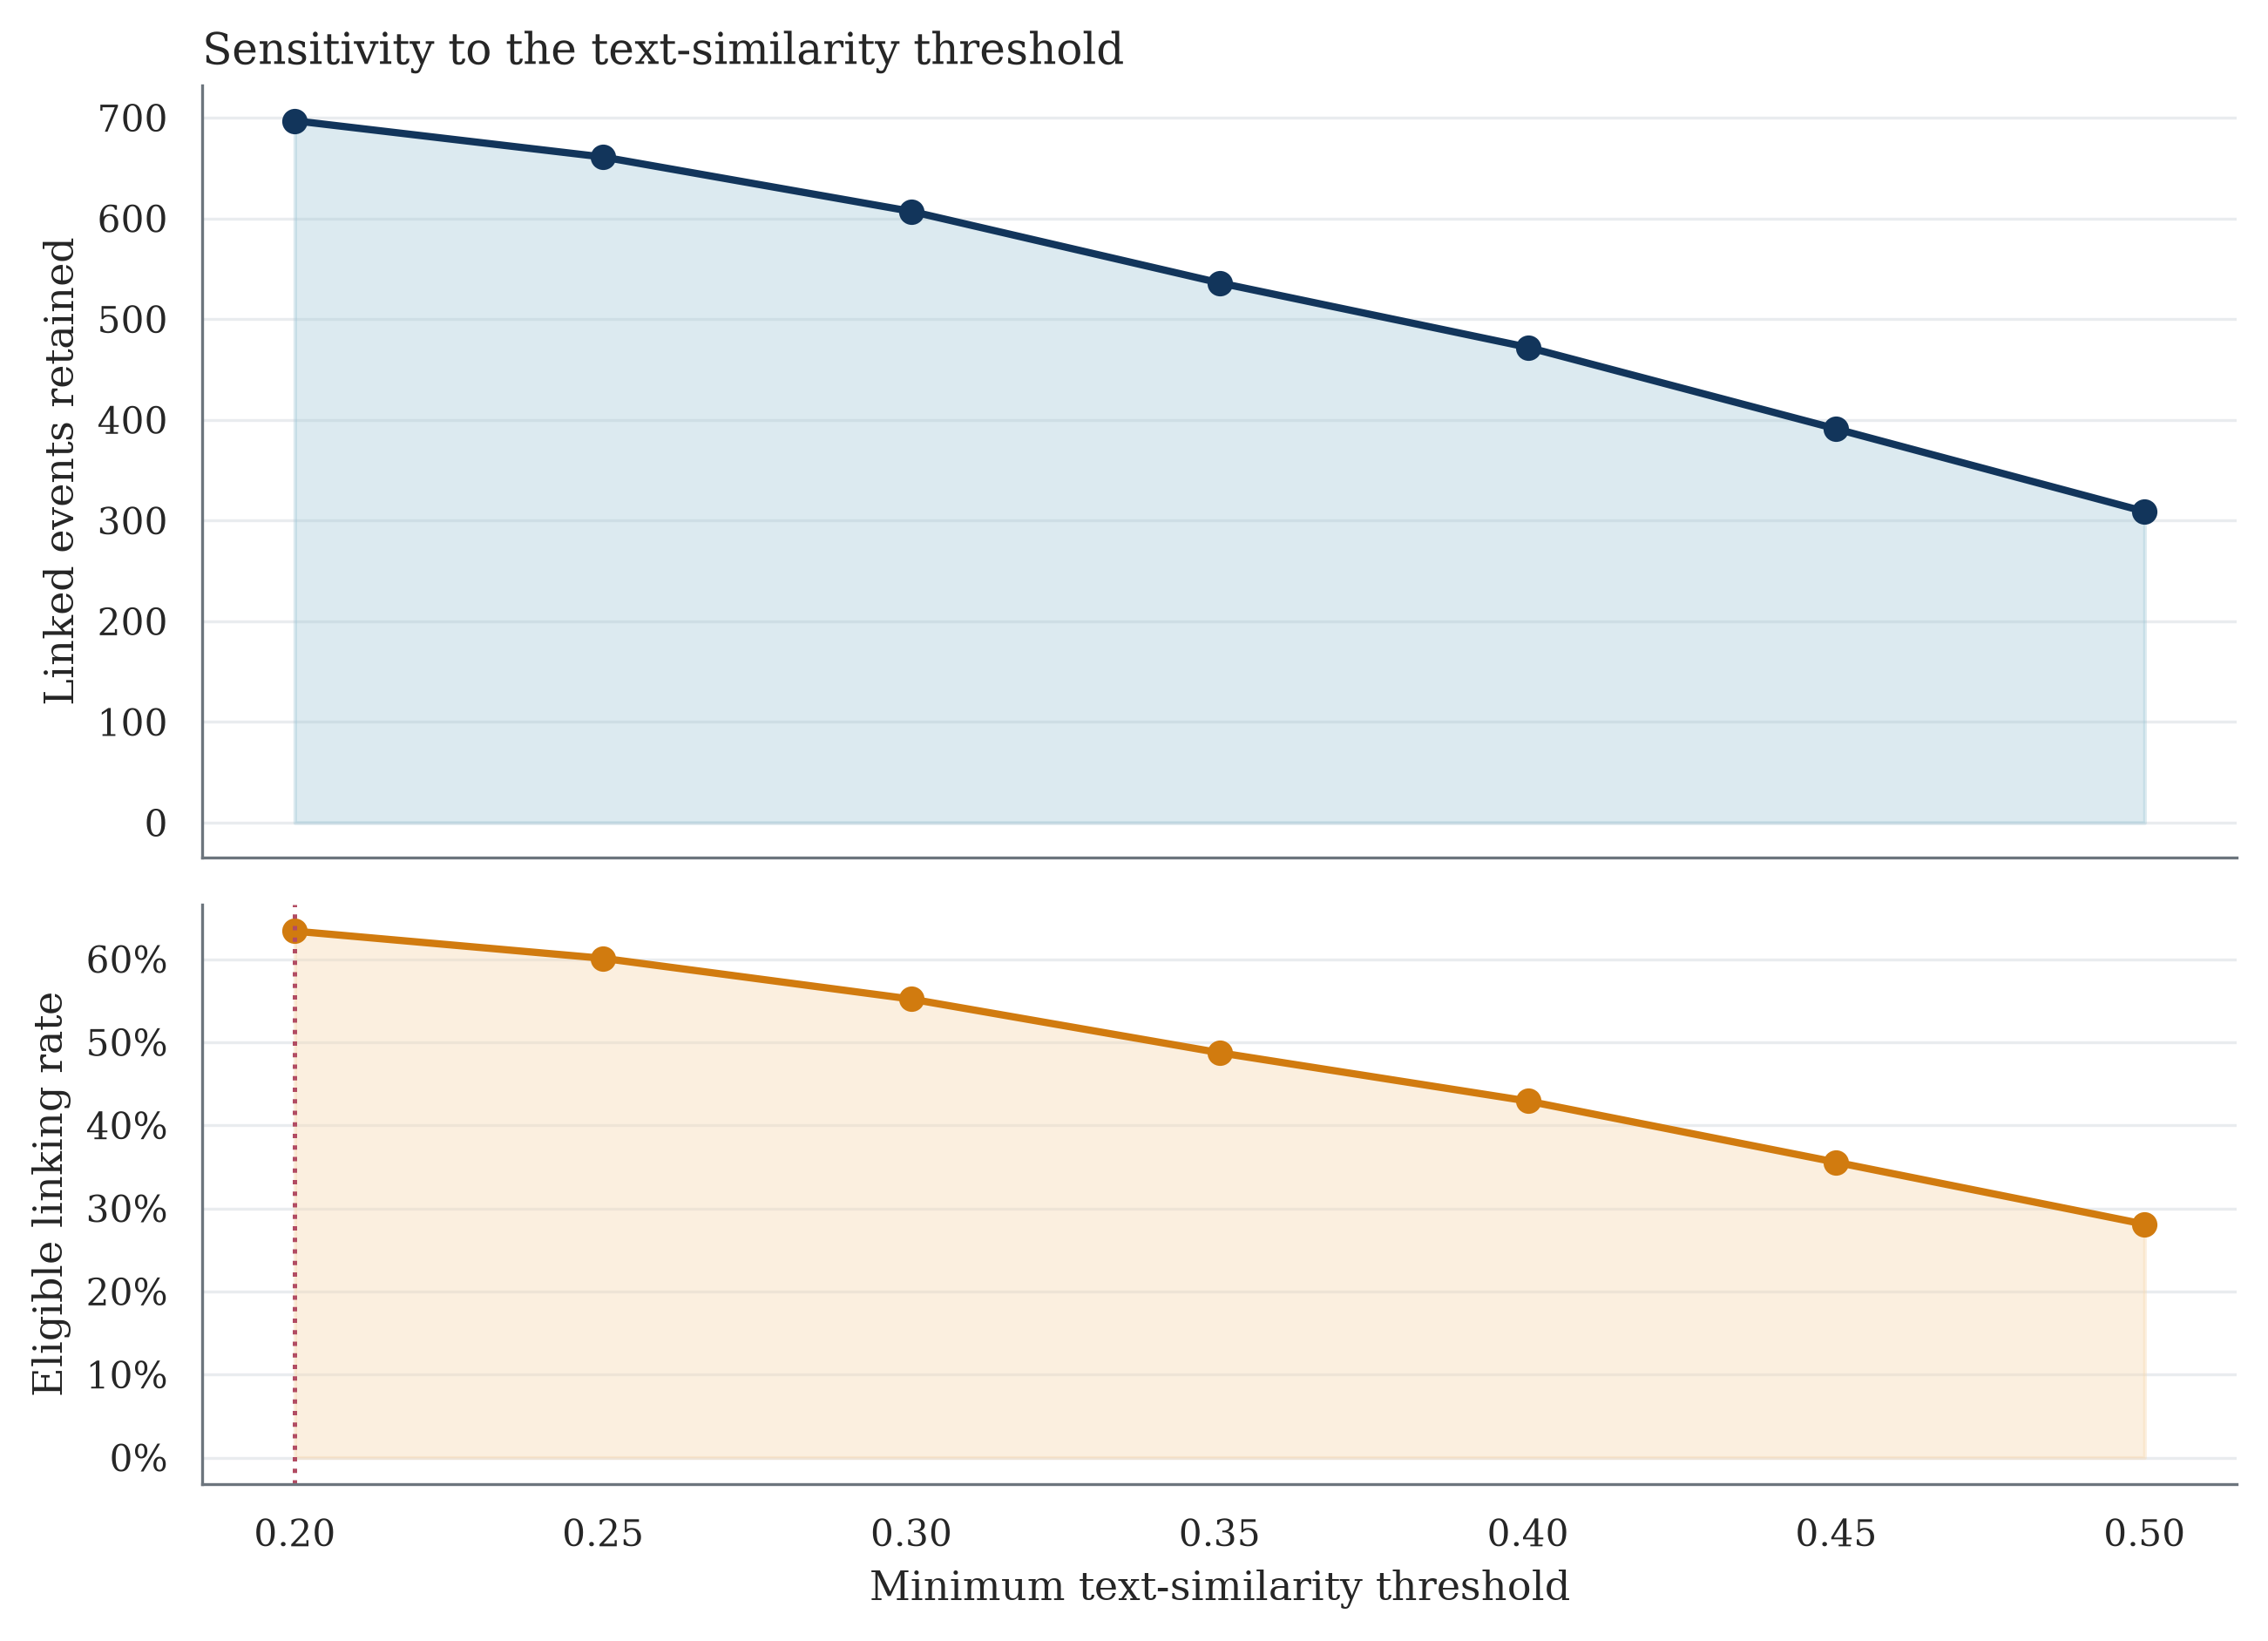
\includegraphics[width=0.82\textwidth]{figures/fig_threshold_sensitivity}
\caption{Number of linked events (blue bars, left axis) and eligible linking
rate (orange line, right axis) as a function of the minimum text-similarity
threshold. At the current threshold of 0.20 (dotted red line), 697 events
are retained (63.4\%). Raising the threshold to 0.30 reduces the count to
607 (55.2\%) and eliminates the 89 pairs with the weakest semantic similarity;
raising it to 0.50 yields 309 events (28.1\%). Note that this 0.50 threshold is
on \emph{text similarity} $s_{\text{text}}$ and is distinct from the Model~B
sensitivity definition in Section~\ref{sec:phase2}, which thresholds the
\emph{composite} score $S(i,j^*) \geq 0.50$ (553 events). This analysis informs the
sensitivity check in Phase~2: the survival model should be run at both 0.20
and 0.30 to assess whether conclusions are stable.}
\label{fig:threshold_sensitivity}
\end{figure}

% =============================================================================
\section{Worked Example}

Table~\ref{tab:example} illustrates the score computation for the first pair in
\texttt{boamp\_renewal\_candidates.csv}.

\begin{table}[h]
\centering
\caption{Score calculation for pair (\texttt{15-31464} $\to$ \texttt{17-176560})}
\label{tab:example}
\begin{tabular}{llr}
\toprule
Quantity & Description & Value \\
\midrule
$t_i$           & Source start date          & 2015-03-02 \\
$d_i$           & Declared duration          & 36 months \\
$\hat{e}_i$     & Estimated end date ($t_i + d_i$) & 2018-03-01 \\
$t_j$           & Candidate start date       & 2017-12-17 \\
$\Delta(i,j)$   & Gap ($t_j - t_i$)          & 33.54 months \\
\midrule
$s_{\text{text}}$ & ST cosine of \textit{objet} embeddings & 0.6922 \\
$s_{\text{cpv}}$  & Source CPV missing $\Rightarrow$ neutral & 0.5000 \\
$s_{\text{temp}}$ & $1 - |33.54 - 36| / 12 = 1 - 2.46/12$ & 0.7951 \\
$s_{\text{buyer}}$& Same buyer group           & 1.0000 \\
\midrule
$S(i,j)$        & $0.40(0.6922) + 0.25(0.5) + 0.20(0.7951) + 0.15(1.0)$ & \textbf{0.7109} \\
\bottomrule
\end{tabular}
\end{table}

\noindent This pair passes both hard filters ($s_{\text{text}} = 0.69 \geq 0.20$;
gap $= 33.5 \in [6, 72]$ months) and is selected as the best match for source
\texttt{15-31464}.

\textbf{Concrete step}

This part illustrates how the renewal-linking score is computed for one
concrete candidate pair. The example comes from the first row of
\texttt{boamp\_renewal\_candidates.csv}.

The source contract is:

\[
\texttt{src} = \texttt{15-31464}
\]

The candidate renewal notice is:

\[
\texttt{cand} = \texttt{17-176560}
\]

Both notices belong to the same buyer group:

\[
\text{Buyer} = \text{D\'epartement de la Mayenne}
\]

\subsection*{Source and Candidate Information}

\begin{table}[h]
\centering
\caption{Source contract and candidate renewal}
\begin{tabular}{lll}
\toprule
Element & Notation & Value \\
\midrule
Source contract ID & $i$ & \texttt{15-31464} \\
Source start date & $t_i$ & 2015-03-02 \\
Declared duration & $d_i$ & 36 months \\
Estimated end date & $\hat{e}_i = t_i + d_i$ & 2018-03 \\
Candidate contract ID & $j$ & \texttt{17-176560} \\
Candidate start date & $t_j$ & 2017-12-17 \\
Buyer match & $b_i = b_j$ & Yes \\
\bottomrule
\end{tabular}
\end{table}

The source contract started on 2015-03-02 and had a declared duration of
36 months. Therefore, the expected renewal date is around March 2018:

\[
\hat{e}_i = 2015\text{-}03\text{-}02 + 36 \text{ months}
\approx 2018\text{-}03
\]

The candidate notice was published on 2017-12-17. This is close to the expected
end date of the original contract, so it is a plausible renewal candidate.

\subsection*{Step 1: Time Gap}

The time gap between the source contract and the candidate is:

\[
\Delta(i,j) = t_j - t_i
\]

In this example:

\[
\Delta(i,j)
=
2017\text{-}12\text{-}17
-
2015\text{-}03\text{-}02
=
33.54 \text{ months}
\]

The declared duration was:

\[
d_i = 36 \text{ months}
\]

So the candidate appears:

\[
36 - 33.54 = 2.46 \text{ months}
\]

before the expected contract end date.

\subsection*{Step 2: Temporal Score}

The temporal score is:

\[
s_{\text{temp}}(i,j)
=
1 -
\frac{|\Delta(i,j) - d_i|}{W}
\]

with:

\[
W = 12
\]

Therefore:

\[
s_{\text{temp}}(i,j)
=
1 -
\frac{|33.54 - 36|}{12}
\]

\[
s_{\text{temp}}(i,j)
=
1 -
\frac{2.46}{12}
\]

\[
s_{\text{temp}}(i,j)
=
0.7951
\]

This is a high temporal score because the candidate appears only about
2.5 months before the expected renewal date.

\subsection*{Step 3: Other Component Scores}

The text similarity score is computed using the cosine similarity between the
two Sentence-Transformer embeddings:

\[
s_{\text{text}}(i,j) = 0.6922
\]

This means that the two contract descriptions are semantically close.

The CPV score is:

\[
s_{\text{cpv}}(i,j) = 0.5
\]

because the source CPV code is missing. The algorithm gives a neutral score
instead of rejecting the pair. This is important because missing CPV should not
automatically imply that two notices are unrelated.

The buyer score is:

\[
s_{\text{buyer}}(i,j) = 1.0
\]

because the two notices belong to the same buyer group.

\subsection*{Step 4: Composite Score}

The composite score is the weighted sum of the four component scores:

\[
S(i,j)
=
0.40s_{\text{text}}
+
0.25s_{\text{cpv}}
+
0.20s_{\text{temp}}
+
0.15s_{\text{buyer}}
\]

Substituting the values:

\[
S(i,j)
=
0.40(0.6922)
+
0.25(0.5)
+
0.20(0.7951)
+
0.15(1.0)
\]

\[
S(i,j)
=
0.2769
+
0.1250
+
0.1590
+
0.1500
\]

\[
S(i,j)
=
0.7109
\]

So the final composite score is:

\[
\boxed{S(i,j) = 0.7109}
\]

This matches the \texttt{composite\_score} reported in the candidate file.

\subsection*{Interpretation}

This pair is considered a plausible renewal link because all main signals are
consistent:

\begin{itemize}
  \item the buyer is the same;
  \item the candidate appears close to the expected contract end date;
  \item the contract descriptions are semantically similar;
  \item the CPV code is missing for the source, but this is treated neutrally
        rather than as evidence against the match.
\end{itemize}

The pair also passes the two hard filters:

\[
s_{\text{text}} = 0.6922 \geq 0.20
\]

and:

\[
\Delta(i,j) = 33.54 \in [6,72]
\]

Therefore, this candidate remains in the filtered candidate set. If it has the
highest composite score among all surviving candidates for source
\texttt{15-31464}, it is selected as the best renewal match:

\[
j^*(i) = \texttt{17-176560}
\]

This example shows exactly how the algorithm transforms raw BOAMP notices into
a renewal-linking score. The score is not legal proof of renewal. It is an
algorithmic measure of plausibility based on buyer identity, timing, text
similarity, and CPV compatibility.

% =============================================================================
\section{Limitations and Risks}

\begin{enumerate}[leftmargin=*, label=\textbf{L\arabic*.}]

  \item \textbf{No explicit ground truth.} BOAMP does not provide a renewal
        field. The \texttt{annonce\_lie} signal on ATTRIBUTION notices
        calibrates text similarity thresholds but is not a direct renewal label.
        The true precision of the 697 links is unknown without manual validation.

  \item \textbf{Name-based buyer fragmentation.} 87.2\% of buyer keys are
        name-based. Variant spellings of the same public entity (abbreviations,
        accents, word order) create separate groups, producing structural false
        negatives that cannot be recovered by tuning thresholds alone.

  \item \textbf{Duration imputation introduces noise, and declared duration is
        an administrative ceiling.} 25.1\% of eligible AO had their duration
        imputed to 48 months. If the true duration differs significantly, the
        temporal window is shifted and the correct renewal candidate may fall
        outside the $\pm$12-month window. More fundamentally, even when duration
        is not imputed, the declared value is the administrative maximum of the
        contract (base period plus all renewal tranches), not the expected actual
        first renewal date. It cannot therefore be used as the survival target.
        See Section~\ref{sec:duration_science} for the full analysis.

  \item \textbf{False positives in sparse-buyer groups.} Relaxing CPV from a
        hard filter to a scored component increases recall but also increases the
        risk of linking two unrelated contracts from the same buyer that happen to
        use similar procurement language (e.g.\ generic IT services descriptions).

  \item \textbf{Sample scope.} The dataset covers only the Pays-de-la-Loire
        region and is focused on ICT/digital services. Linking rates and score
        distributions may differ significantly for other regions or sectors.

\end{enumerate}

% =============================================================================
\clearpage
\section{Dataset Reliability Analysis}
\label{sec:reliability}

This section consolidates the quantitative reliability checks performed on
\texttt{boamp\_renewal\_links.csv} before it is used as input to the survival
model. The goal is to characterise the confidence gradient across the 697
linked pairs and provide a principled basis for the threshold sensitivity
analysis recommended in Phase~2.

\subsection{Confidence Tiers}

Each linked contract is assigned to one of three confidence tiers based on its
composite score $S(i,j^*)$:

\begin{table}[H]
\centering
\caption{Confidence tiers for linked contracts (event = 1, $n = 697$)}
\begin{tabular}{lccc}
\toprule
Tier & Criterion & Count & Share \\
\midrule
HIGH   & $S(i,j^*) \geq 0.70$ & 205 & 29.4\% \\
MEDIUM & $0.50 \leq S(i,j^*) < 0.70$ & 348 & 49.9\% \\
LOW    & $S(i,j^*) < 0.50$ & 144 & 20.7\% \\
\midrule
\multicolumn{2}{l}{Censored (event = 0)} & 403 & --- \\
\bottomrule
\end{tabular}
\end{table}

\begin{figure}[H]
\centering
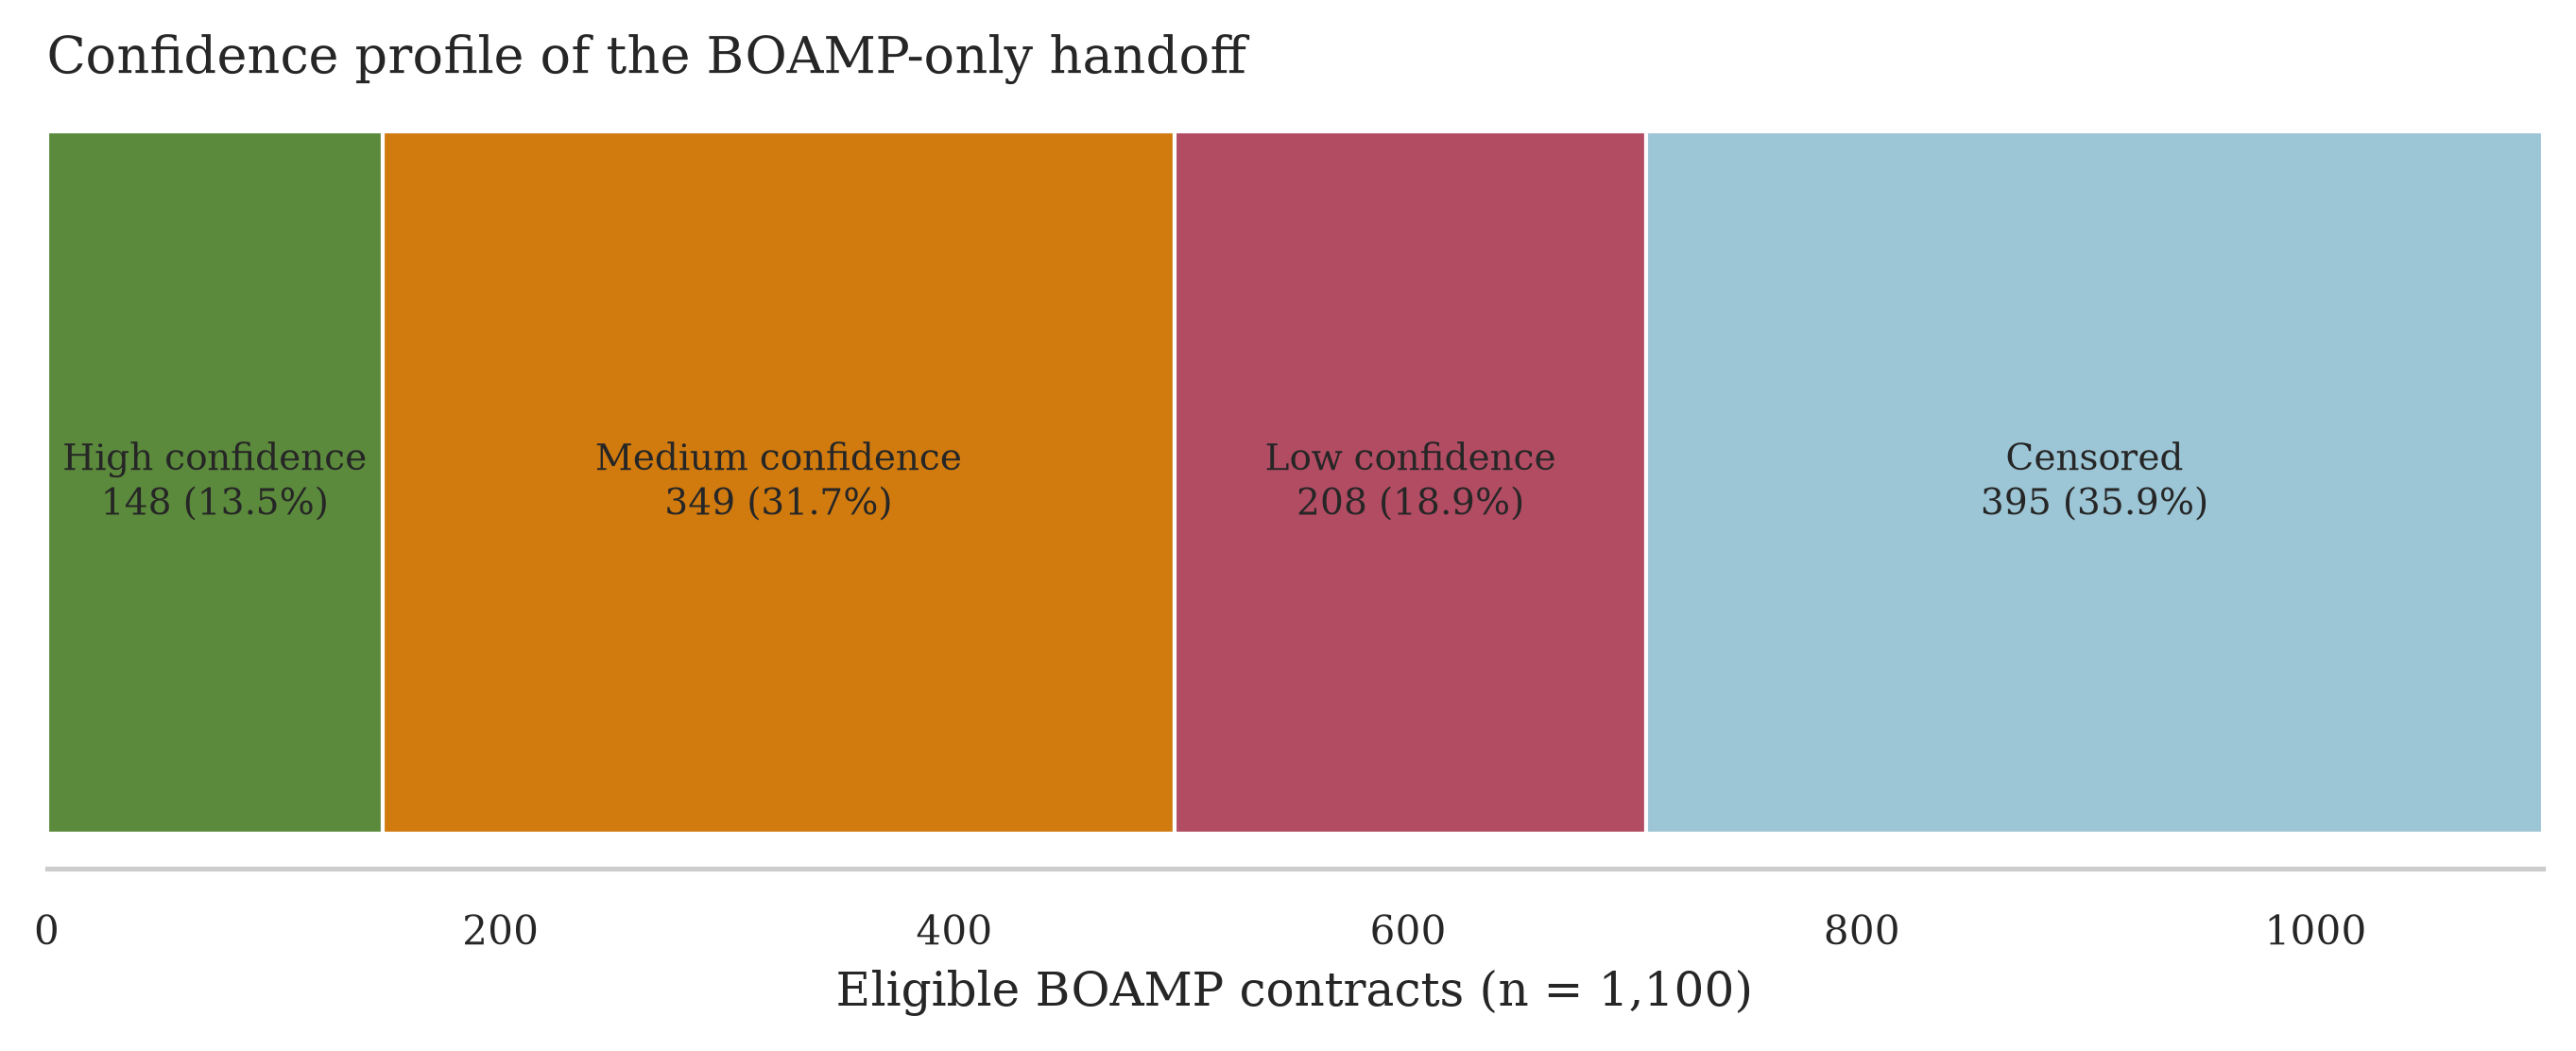
\includegraphics[width=0.90\textwidth]{figures/fig_confidence_tiers}
\caption{Confidence tier breakdown across all 1,100 eligible contracts. Green
= HIGH ($S \geq 0.70$, $n = 205$); orange = MEDIUM ($0.50 \leq S < 0.70$,
$n = 348$); red = LOW ($S < 0.50$, $n = 144$); light blue = censored
(event = 0, $n = 403$). The HIGH and MEDIUM tiers together cover 553 of the
697 linked contracts (79.3\%), providing a reliable core dataset for survival
modeling. LOW-tier links represent the greatest false-positive risk and should
be downgraded to censored in the sensitivity check.}
\label{fig:confidence_tiers}
\end{figure}

For the survival model in Phase~2, the recommended protocol is:

\begin{enumerate}
  \item \textbf{Primary model}: all 697 events (composite $\geq 0.20$, text $\geq 0.20$).
  \item \textbf{Sensitivity check}: 553 events only (drop LOW tier, i.e.\ composite $\geq 0.50$).
  \item If hazard ratios and survival curve shapes are stable between the two
        runs, the LOW-confidence links are not distorting conclusions --- they add noise
        but not bias. If results change substantially, report the sensitivity-check
        model as the primary.
\end{enumerate}

\subsection{Score Disambiguation: Margin Between Best and Second-Best Candidate}

For source contracts that had more than one candidate, the margin between the
best and second-best composite score measures how clearly the algorithm resolved
the ambiguity. A small margin (best $\approx$ second-best) indicates that an
alternative renewal link was nearly as plausible as the selected one.

\begin{figure}[H]
\centering
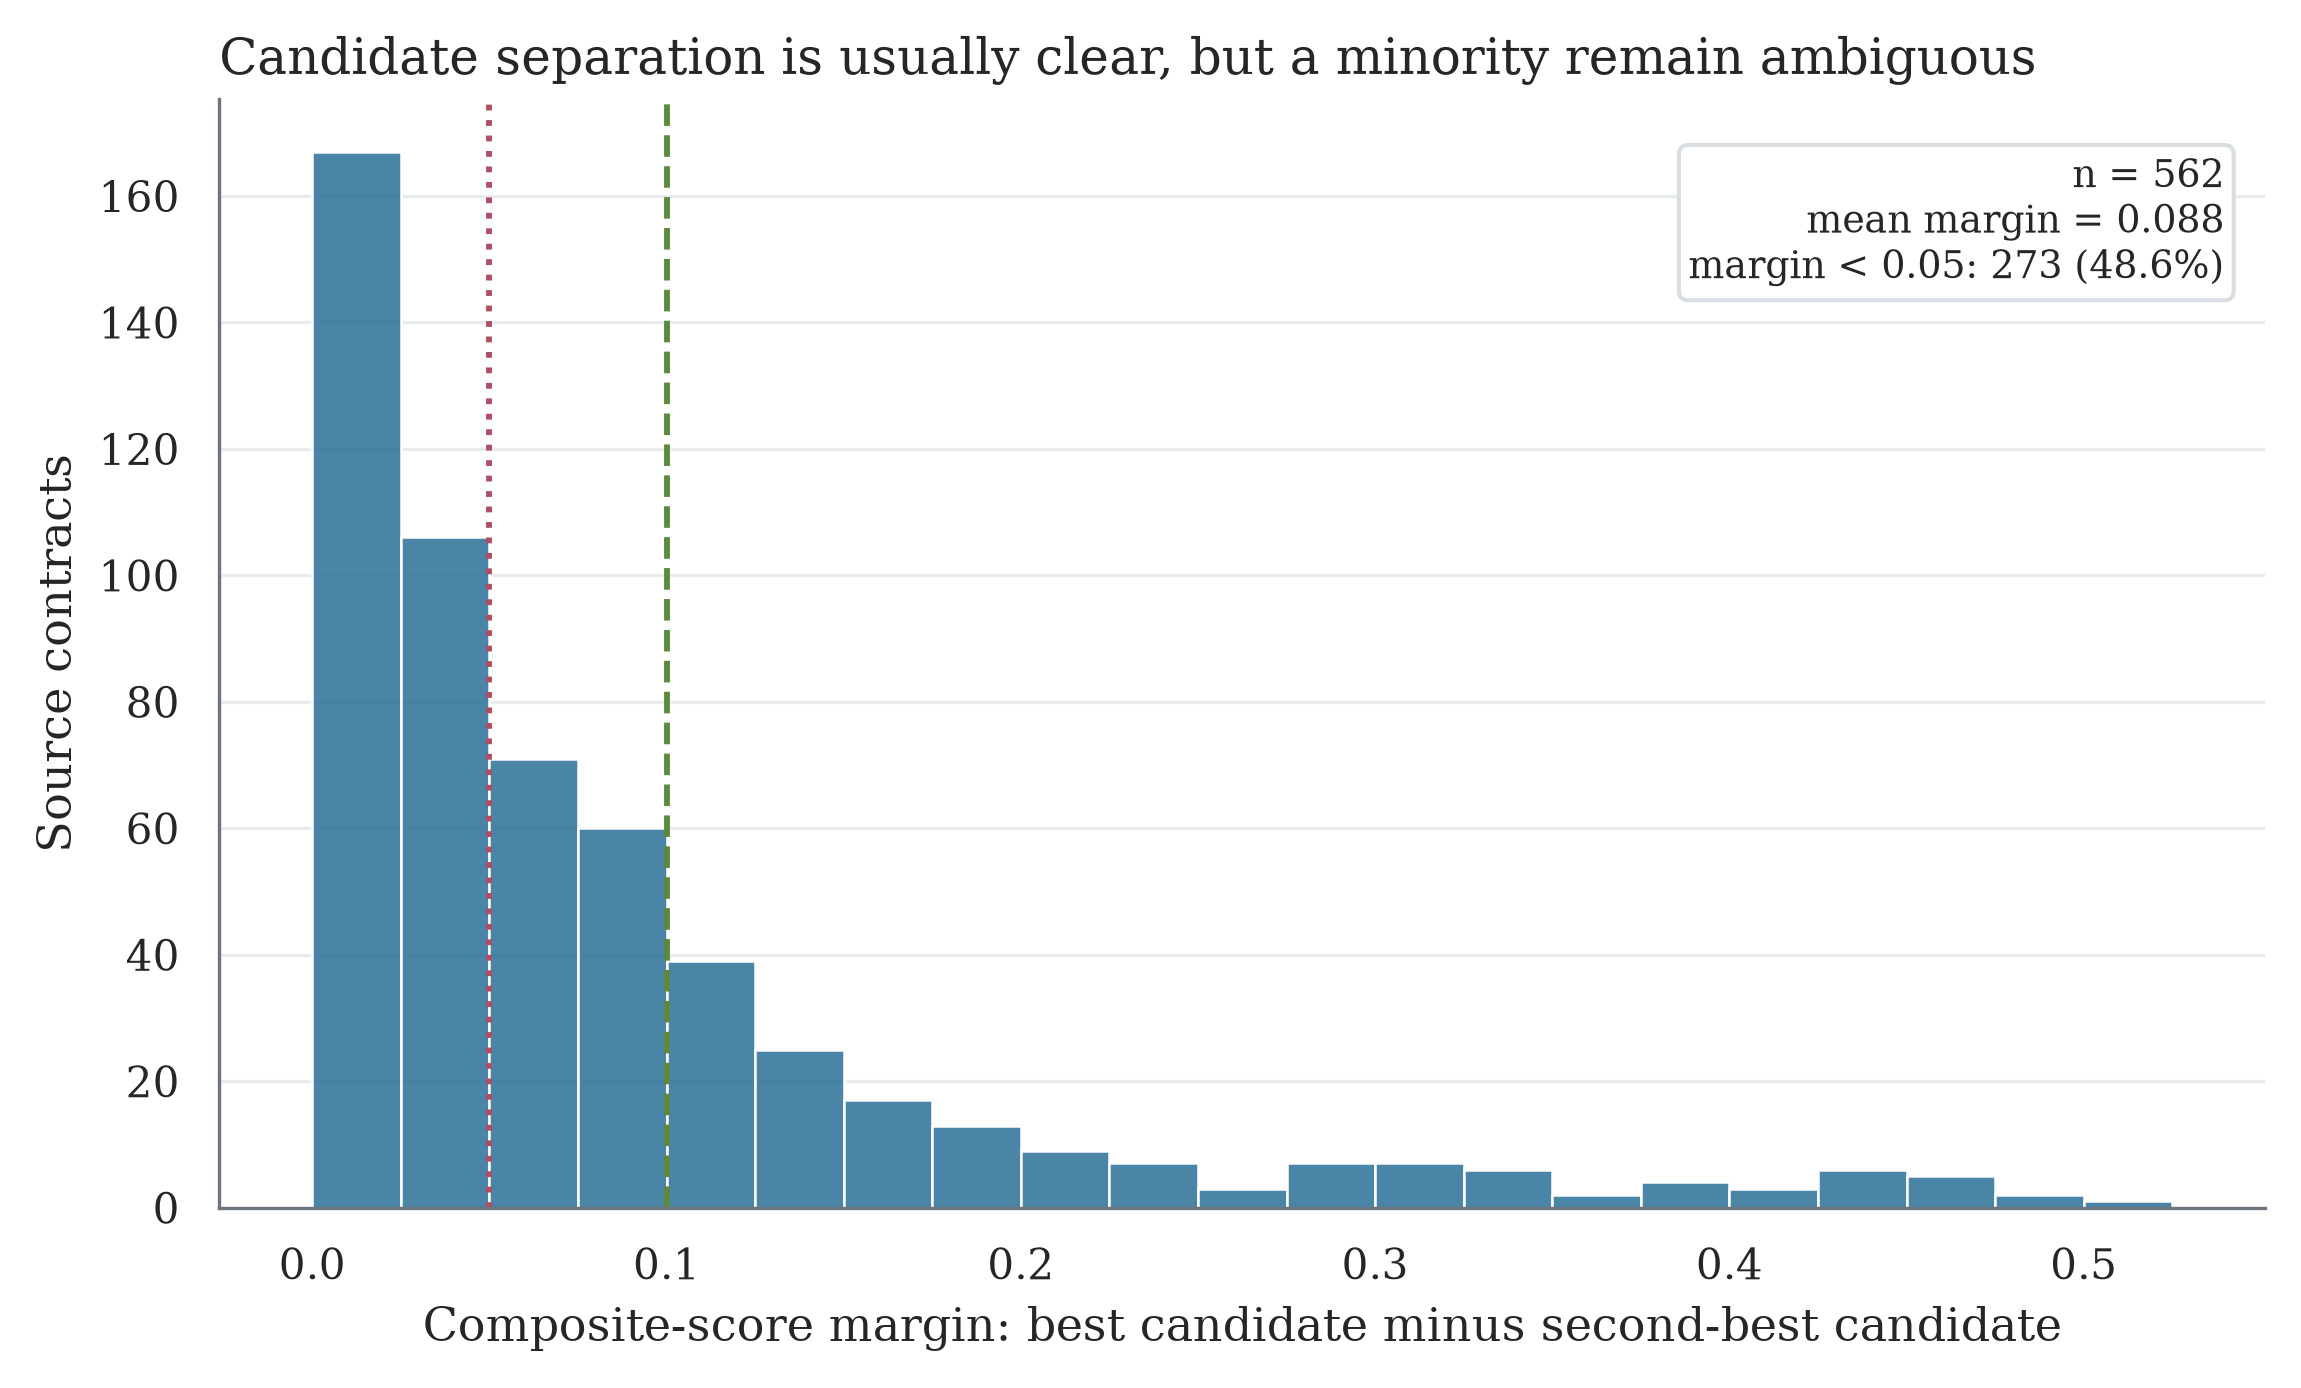
\includegraphics[width=0.82\textwidth]{figures/fig_score_margin}
\caption{Distribution of the score margin (best composite $-$ second-best
composite) for the 562 multi-candidate source contracts. The dotted red line
marks the 0.05 threshold below which 44.7\% of pairs are considered
\textit{ambiguous}: the algorithm selected one candidate, but an alternative
was within 0.05 of the same score. The dashed green line at 0.10 marks the
\textit{clear winner} zone (27.9\% of pairs). These ambiguous pairs are
concentrated in the LOW and MEDIUM confidence tiers and are the primary
motivation for the manual validation sample recommended in Section~11.}
\label{fig:score_margin}
\end{figure}

The 44.7\% ambiguous-margin rate does not mean the algorithm chose wrongly in
those cases --- it means the available signals were not strong enough to
distinguish the best candidate from the runner-up with high certainty. This is
a structural property of the data (multiple contracts from the same buyer in
similar time windows) and cannot be resolved by tuning thresholds. Manual
validation of a stratified sample is the appropriate mitigation.

\subsection{Ground-Truth Calibration}

An indirect calibration is possible using the \texttt{annonce\_lie} field on
ATTRIBUTION notices. These notices back-reference the original call-for-tender,
providing external evidence of real procurement activity on those AO records.
Among the 466 eligible AO notices that are referenced by at least one
ATTRIBUTION notice, 318 were linked (68.2\%), compared to 63.4\% overall.
The algorithm performs \textit{better} on contracts with external evidence of
activity, which is the expected direction.

\subsection{Summary of Reliability Findings}

\clearpage
\begin{landscape}
\thispagestyle{empty}
\begin{table}[p]
\centering
\caption{Reliability check results for \texttt{boamp\_renewal\_links.csv}}
\small
\begin{tabularx}{\linewidth}{@{}X P{4.2cm} X@{}}
\toprule
Check & Result & Interpretation \\
\midrule
Internal integrity (duplicates, impossible values) & All clean & No structural data errors \\[4pt]
Hard-filter compliance (all event=1 in [6,72] mo) & 100\% compliant & Algorithm applied correctly \\[4pt]
Temporal error mean (observed $-$ declared) & $-0.04$ months & No systematic temporal bias \\[4pt]
Temporal error std & 4.87 months & Tight; consistent with $\pm$12 mo window \\[4pt]
Duration imputed vs.\ non-imputed $|$error$|$ & 4.1 vs.\ 3.7 mo & Negligible difference \\[4pt]
Year-by-year rate stability (2015--2022) & 50--75\% & Stable; 2023 drop is structural \\[4pt]
\texttt{annonce\_lie} calibration & 68.2\% vs.\ 63.4\% & Positive signal \\[4pt]
Low text-similarity links ($s_{\text{text}} < 0.30$) & 89 pairs (12.8\%) & Highest false-positive risk \\[4pt]
Ambiguous score margin ($<0.05$) & 44.7\% of multi-cand. & Structural; not tunable \\[4pt]
HIGH + MEDIUM tier share & 553 / 697 (79.3\%) & Reliable core for modeling \\
\bottomrule
\end{tabularx}
\normalsize
\end{table}
\end{landscape}
\clearpage

% =============================================================================
\clearpage
\section{Output Files Summary}

\noindent The notebook produces five output files (four in the \texttt{outputs/}
directory plus the \texttt{boamp\_phase2\_survival.csv} handoff). The main modeling table is
the renewal links file. The other files preserve candidate pairs, aggregate
linking statistics, and diagnostic failure patterns for audit and sensitivity
analysis.

\begin{table}[H]
\centering
\caption{Output files produced by the BOAMP linking workflow}
\small
\begin{tabular}{@{}P{6.4cm}R{1.2cm}P{6.4cm}@{}}
\toprule
File & Rows & Purpose \\
\midrule
\texttt{boamp\_renewal\_links.csv}      & 1,100 & Notebook linking output. One row per eligible AO before final handoff standardisation. \\
\texttt{boamp\_phase2\_survival.csv}    & 1,100 & \textbf{Official modeling input.} BOAMP-only handoff with explicit renewal and censoring duration columns. \\
\texttt{boamp\_renewal\_candidates.csv} & 5,356 & All filtered candidate pairs before best-match selection. Useful for threshold sensitivity analysis. \\
\texttt{boamp\_linking\_stats.csv}      & 1     & Summary statistics: total AO, eligible, linked, linking rate. \\
\texttt{boamp\_bias\_report.csv}        & 62    & Failure reason $\times$ CPV cross-tabulation. Diagnoses which categories are under-linked. \\
\bottomrule
\end{tabular}
\normalsize
\end{table}

% =============================================================================
\section{Phase 2 --- Survival Analysis}
\label{sec:phase2}

Phase 2 fits survival models on \texttt{boamp\_phase2\_survival.csv}, the
official BOAMP-only handoff produced by Phase 1. The survival time is
\texttt{observed\_duration\_months} ($= \Delta(i, j^*)$ for linked contracts;
time-to-study-end for censored ones). The event indicator is \texttt{event}
(1 = renewal linked, 0 = right-censored).

\subsection{Dataset Overview}

\begin{table}[H]
\centering
\caption{Phase 2 dataset summary (\texttt{boamp\_phase2\_survival.csv})}
\begin{tabular}{lr}
\toprule
Metric & Value \\
\midrule
Total contracts (rows)          & 1,100 \\
Events (\texttt{event = 1})     & 697 (63.4\%) \\
Censored (\texttt{event = 0})   & 403 (36.6\%) \\
Median observed duration (all)  & 46.8 months \\
Median renewal gap (events)     & 37.0 months \\
Study period                    & 2015-03-02 to 2024-12-29 \\
\bottomrule
\end{tabular}
\end{table}

\subsection{Statistical Methods and Notation}
\label{sec:phase2_methods}

Let $Y_i$ denote the Phase 1 algorithmic linking outcome. In Phase 2, the
standard survival-analysis event indicator is defined as $\delta_i = Y_i$.
Thus $\delta_i = 1$ means that an identifiable BOAMP renewal was linked by the
algorithm, and $\delta_i = 0$ means that no renewal was observed under the
available data and matching rule.

Let $T_i$ denote the latent time-to-identifiable BOAMP renewal (in months) for contract $i$ and
$C_i$ the censoring time (time from contract start to end of study period for
right-censored observations). What is observed is the pair
$(T_i^{\text{obs}},\, \delta_i)$ where:

\begin{equation}
  T_i^{\text{obs}} = \min(T_i,\, C_i),
  \qquad
  \delta_i = \mathbf{1}[T_i \leq C_i].
\end{equation}

In the output file, $T_i^{\text{obs}}$ is stored in
\texttt{observed\_duration\_months} and $\delta_i$ in \texttt{event}.

\paragraph{Kaplan--Meier estimator.}
Let $t_1 < t_2 < \cdots < t_k$ be the distinct observed event times, $d_j$ the
number of events at time $t_j$, and $n_j$ the number of contracts at risk just
before $t_j$. The product-limit estimator of the survival function is:

\begin{equation}
  \hat{S}(t) = \prod_{j:\, t_j \leq t} \left(1 - \frac{d_j}{n_j}\right).
\end{equation}

\paragraph{Log-rank test.}
For two strata, the log-rank statistic can be written as:

\begin{equation}
  \chi^2_{\text{LR}}
  =
  \frac{\left(\sum_j (O_{1j} - E_{1j})\right)^2}
       {\sum_j V_{1j}},
\end{equation}

where $O_{1j}$ is the observed and $E_{1j}$ the expected number of events in
stratum 1 at time $t_j$, and $V_{1j}$ is the hypergeometric variance. For
$K>2$ strata, the test generalises to a vector/matrix form and follows a
$\chi^2$ distribution with $K - 1$ degrees of freedom under the null hypothesis
of equal survival.

\paragraph{Cox proportional hazards model.}
The hazard function for contract $i$ with covariate vector $\mathbf{x}_i$ is:

\begin{equation}
  h(t \mid \mathbf{x}_i)
  =
  h_0(t)\,\exp\!\bigl(\boldsymbol{\beta}^\top \mathbf{x}_i\bigr),
\end{equation}

where $h_0(t)$ is an unspecified baseline hazard. Parameters $\boldsymbol{\beta}$
are estimated by maximising the partial likelihood. For readability, the
no-ties form is:

\begin{equation}
  \mathcal{L}(\boldsymbol{\beta})
  =
  \prod_{i:\,\delta_i = 1}
  \frac{\exp\!\bigl(\boldsymbol{\beta}^\top \mathbf{x}_i\bigr)}
       {\displaystyle\sum_{j \in \mathcal{R}(T_i^{\text{obs}})}
        \exp\!\bigl(\boldsymbol{\beta}^\top \mathbf{x}_j\bigr)},
\end{equation}

where $\mathcal{R}(t) = \{j : T_j^{\text{obs}} \geq t\}$ is the risk set at
time $t$. The hazard ratio for covariate $k$ is $\mathrm{HR}_k = \exp(\beta_k)$;
a value $> 1$ indicates a higher instantaneous renewal rate (faster renewal).
Because the empirical durations are measured in months, tied event times can
occur; the software implementation handles ties internally.
All Cox and AFT models are fitted with a small ridge ($L_2$) penalty of
$\lambda = 0.1$ on the coefficients (the lifelines \texttt{penalizer}
parameter). This stabilises estimation in the presence of correlated dummy
covariates and mildly shrinks the reported hazard ratios and confidence
intervals toward the null; exact reproduction of the tabulated values requires
the same penalty.

\paragraph{Concordance index (C-index).}
In-sample ranking ability is measured by Harrell's C-index:

\begin{equation}
  C
  =
  \frac{
    \displaystyle\sum_{(i,j):\, T_i^{\text{obs}} < T_j^{\text{obs}},\; \delta_i = 1}
    \mathbf{1}\bigl[\hat{\eta}_i > \hat{\eta}_j\bigr]
  }{
    \displaystyle\sum_{(i,j):\, T_i^{\text{obs}} < T_j^{\text{obs}},\; \delta_i = 1}
    1
  },
\end{equation}

where $\hat{\eta}_i = \boldsymbol{\hat{\beta}}^\top \mathbf{x}_i$ is the
estimated linear predictor. $C = 0.5$ corresponds to random ranking;
$C = 1$ is perfect discrimination.

\paragraph{Accelerated failure time (AFT) models.}
Parametric AFT models assume:

\begin{equation}
  \log T_i = \mu + \boldsymbol{\gamma}^\top \mathbf{x}_i + \sigma \epsilon_i,
\end{equation}

where the distribution of $\epsilon_i$ determines the model family:

\begin{equation}
  \epsilon_i \sim
  \begin{cases}
    \mathcal{N}(0,1)  & \text{log-normal} \\
    \text{Logistic}(0,1) & \text{log-logistic} \\
    \text{Gumbel}(0,1) & \text{Weibull}
  \end{cases}
\end{equation}

Parameters $(\mu, \boldsymbol{\gamma}, \sigma)$ are estimated by maximum
likelihood with right-censored observations. Model selection uses the
Akaike Information Criterion:

\begin{equation}
  \mathrm{AIC} = -2\,\hat{\ell} + 2p,
\end{equation}

where $\hat{\ell}$ is the maximised log-likelihood and $p$ is the number of
free parameters.

\paragraph{Proportional hazards assumption.}
The PH assumption requires $h(t \mid \mathbf{x}_i) / h(t \mid \mathbf{x}_j)$
to be constant over time. A graphical check uses the log-log transformation:
if the PH assumption holds, $\log(-\log\hat{S}_k(t))$ curves across strata
$k$ should be approximately parallel.

\subsection{Kaplan--Meier Survival Estimates}

\subsubsection*{Global Kaplan--Meier Curve}

Figure~\ref{fig:km_global} shows the overall survival function estimated from
all 1,100 contracts. The global KM median survival is \textbf{48.0 months},
consistent with the dominant 48-month administrative duration cluster in the
declared duration distribution. The 95\% confidence interval widens beyond
60 months as fewer contracts remain at risk.

\begin{figure}[H]
\centering
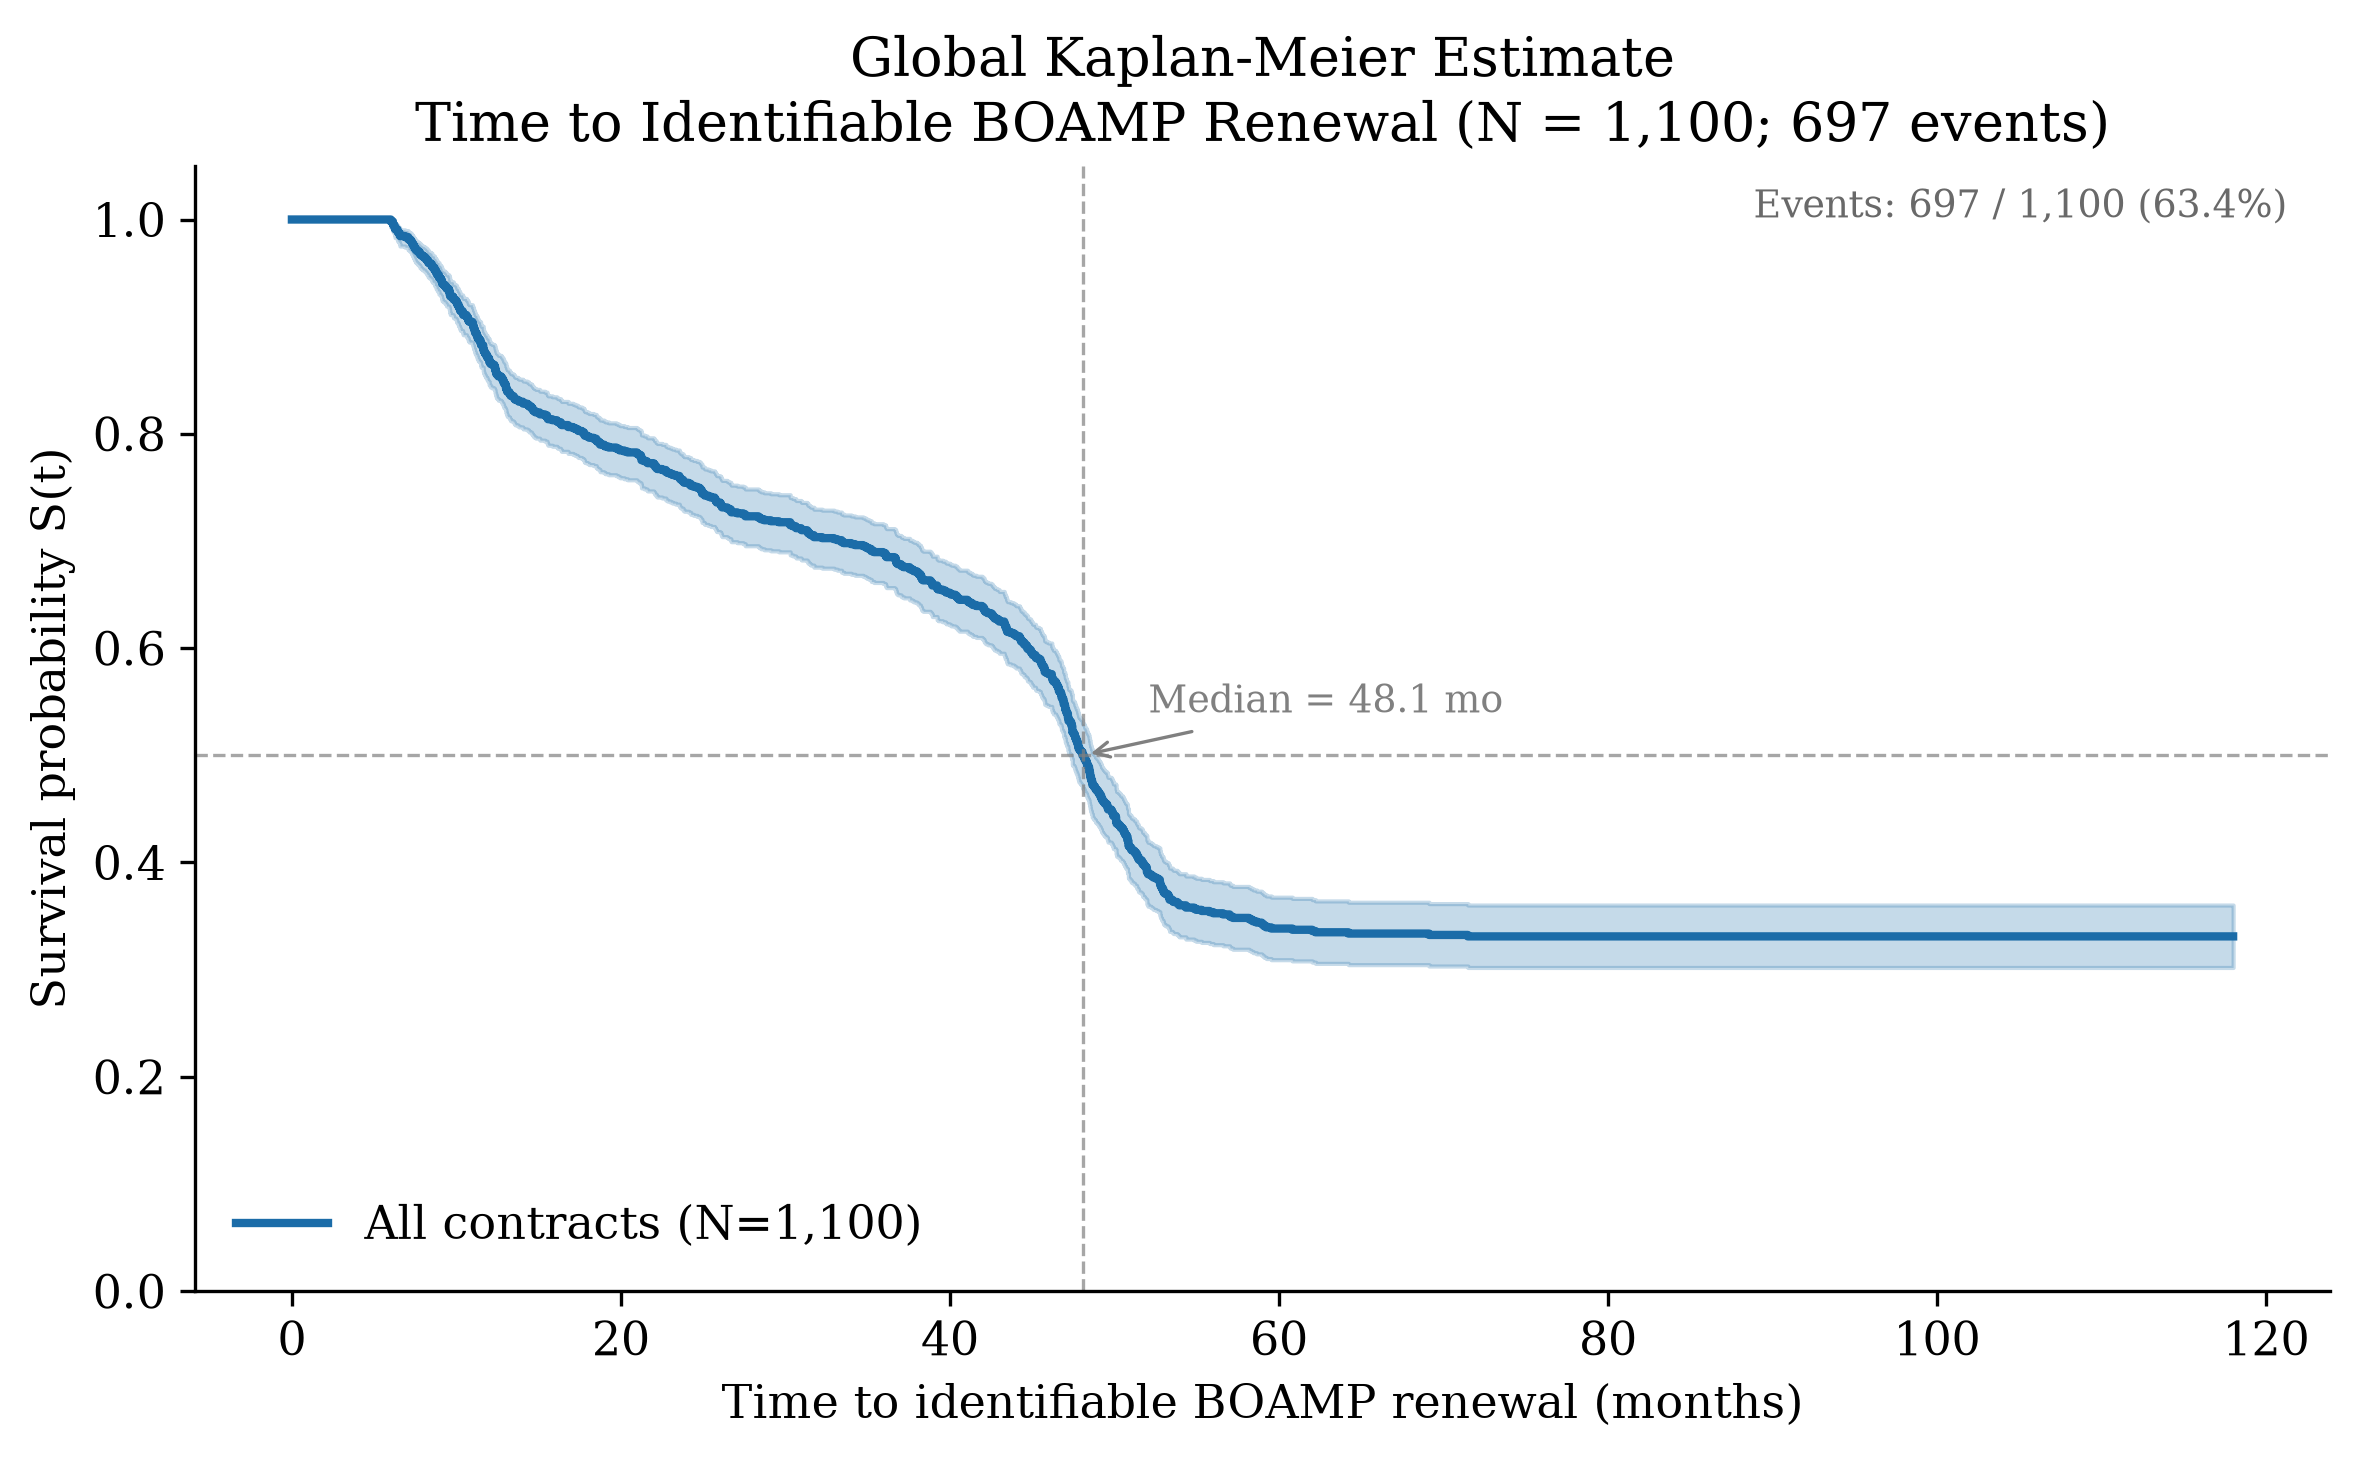
\includegraphics[width=0.88\textwidth]{figures/survival/km_global}
\caption{Global Kaplan--Meier survival curve for all 1,100 eligible contracts.
The solid blue line is the KM estimate; the shaded band is the 95\% pointwise
confidence interval. Censored observations are marked by tick marks.
Median survival = 48.0 months (vertical dashed line).}
\label{fig:km_global}
\end{figure}

\subsubsection*{Stratified Kaplan--Meier Curves}

\paragraph{By service category.}
Figure~\ref{fig:km_category} stratifies the KM curve by the five most
represented service categories (Cybersecurity, IT Services \& Consulting,
Software \& Applications, Telecom \& Networks, and Other). The log-rank test
gives a test statistic of 6.23 ($p = 0.182$, $\mathrm{df} = 4$), indicating
no statistically significant difference in renewal timing across ICT categories
at the 5\% level.

\begin{figure}[H]
\centering
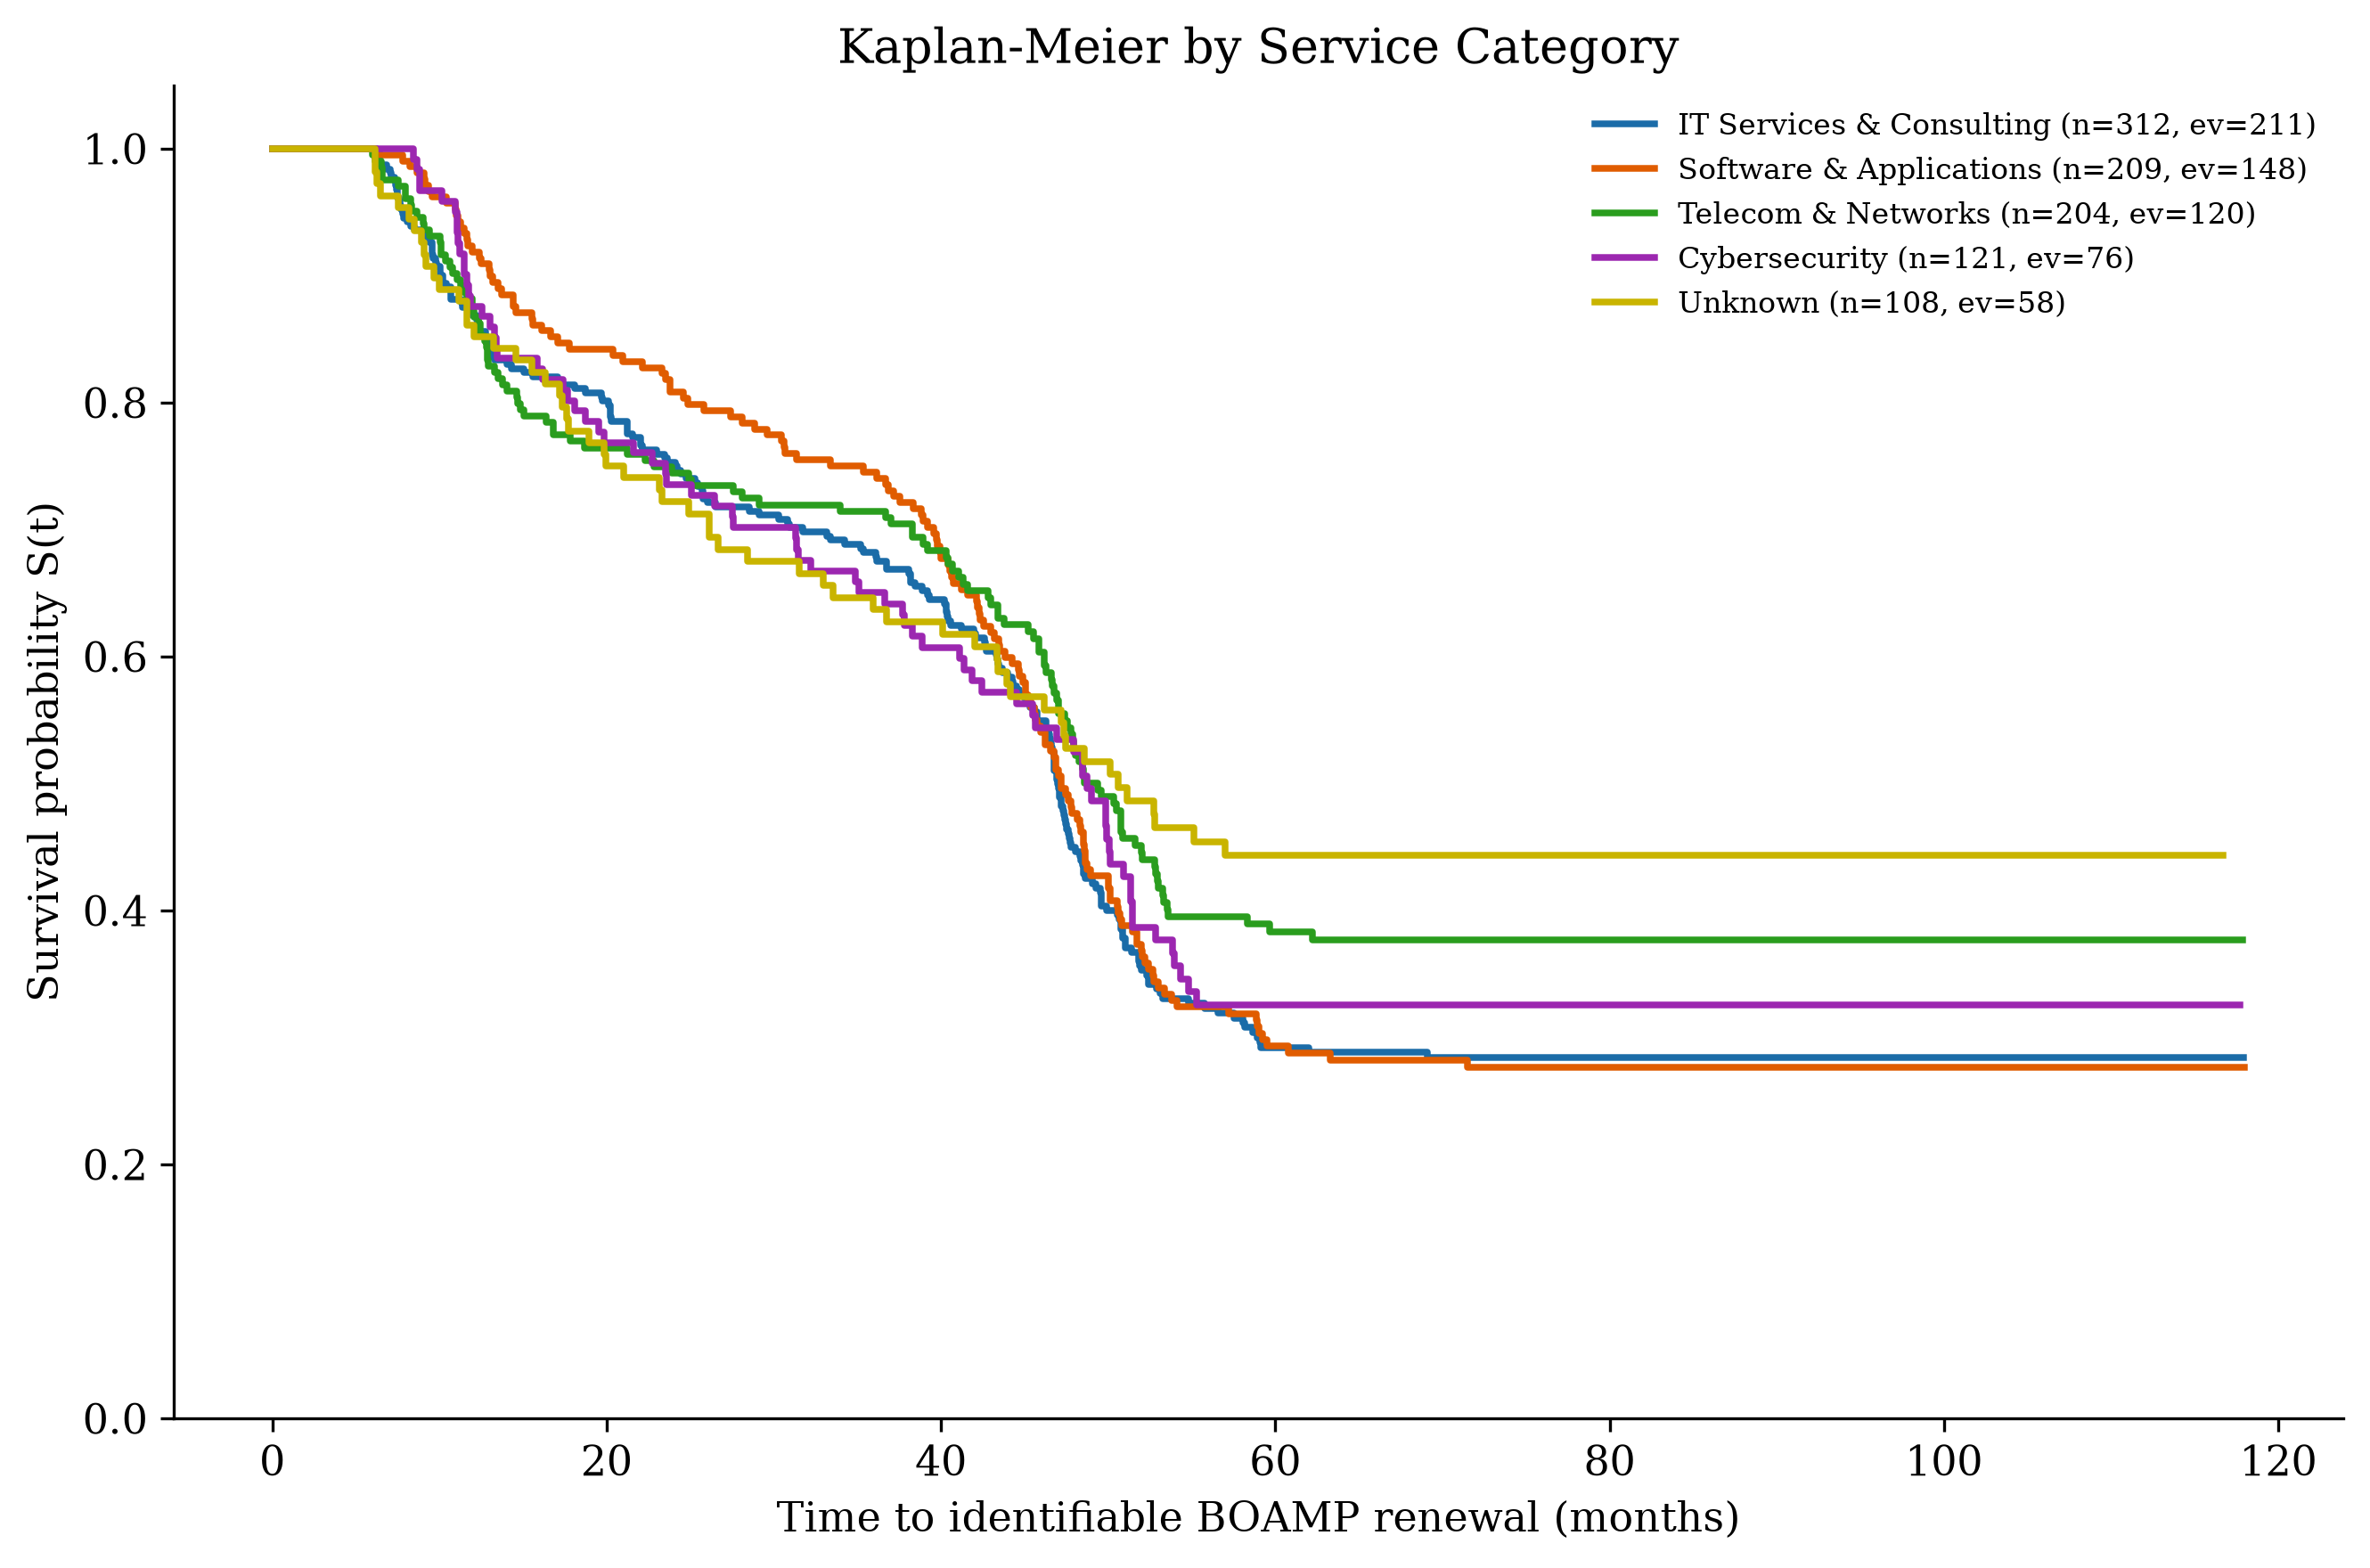
\includegraphics[width=0.88\textwidth]{figures/survival/km_by_category}
\caption{Kaplan--Meier survival curves stratified by service category.
Log-rank test: $\chi^2 = 6.23$, $p = 0.182$, $\mathrm{df} = 4$.
No category shows a statistically significant difference in time-to-renewal.}
\label{fig:km_category}
\end{figure}

\paragraph{By declared duration group.}
Figure~\ref{fig:km_duration} stratifies contracts into three duration bins:
$\leq 24$ months, 25--48 months, and $> 48$ months. The log-rank test
gives $\chi^2 = 62.30$ ($p \approx 0$, $\mathrm{df} = 2$), confirming that
declared contract duration is the strongest predictor of renewal timing --- as
expected, since it defines the temporal search window.

\begin{figure}[H]
\centering
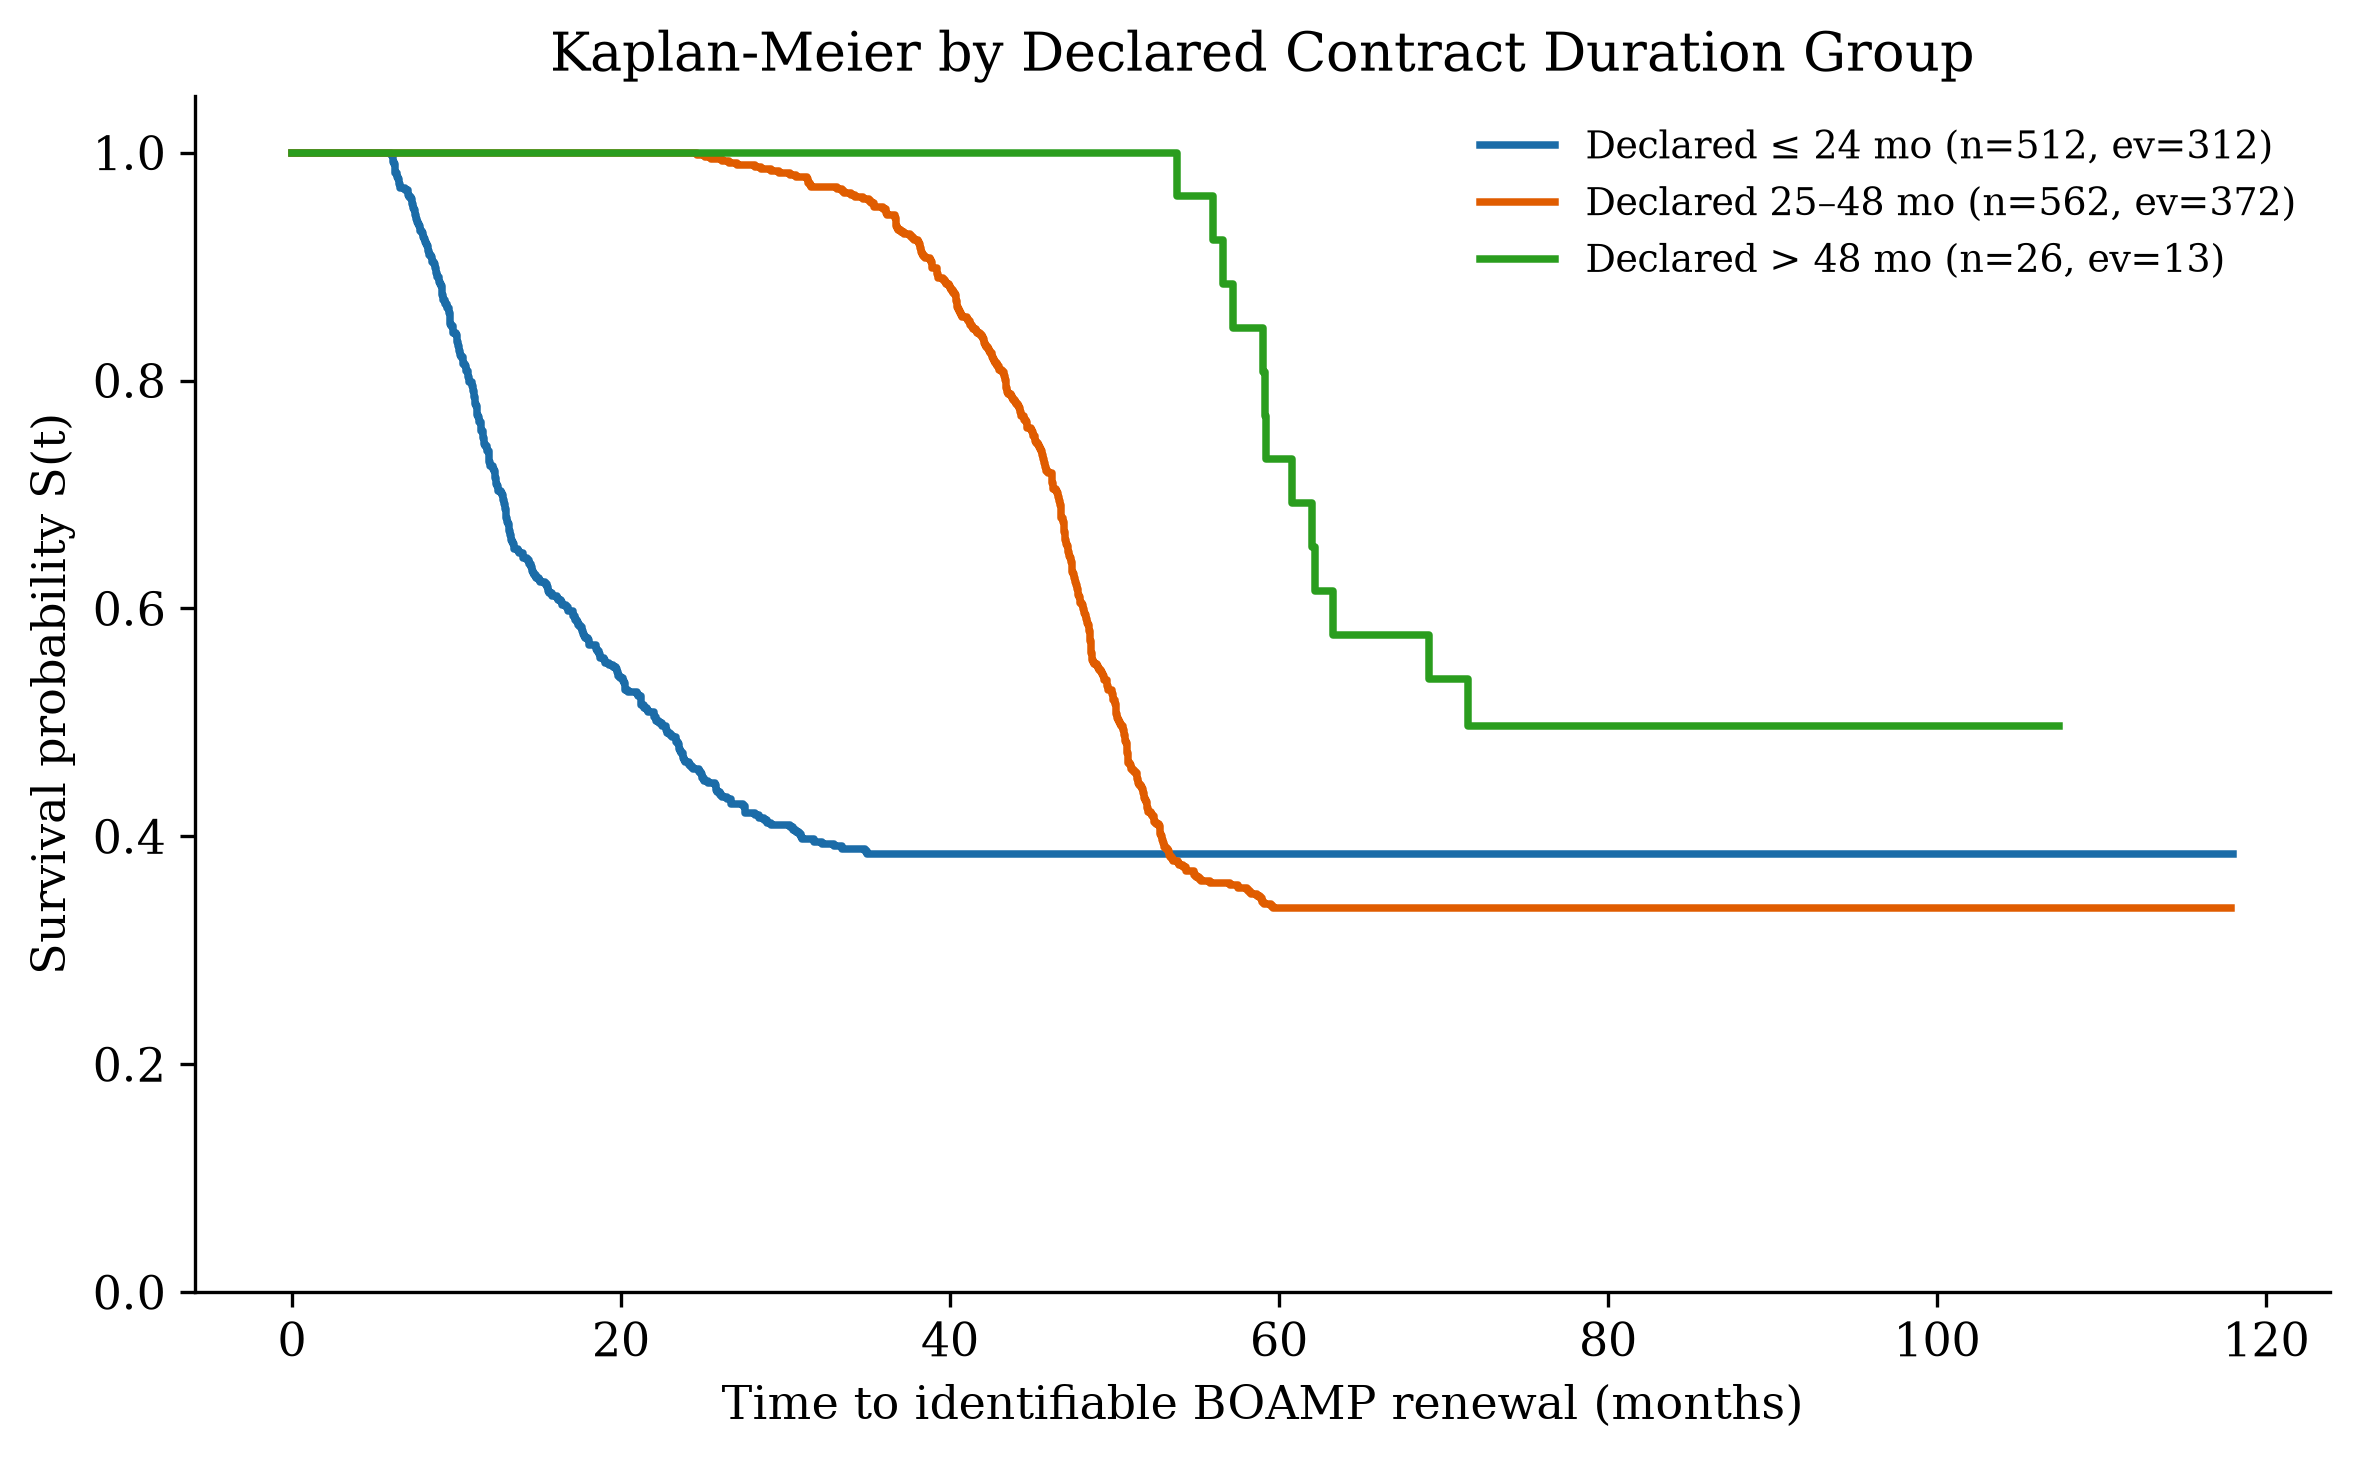
\includegraphics[width=0.88\textwidth]{figures/survival/km_by_declared_group}
\caption{Kaplan--Meier survival curves stratified by declared duration group
($\leq 24$ mo, 25--48 mo, $> 48$ mo).
Log-rank test: $\chi^2 = 62.30$, $p \approx 0$, $\mathrm{df} = 2$.
Shorter declared durations are associated with earlier renewal events.}
\label{fig:km_duration}
\end{figure}

\paragraph{By imputation status.}
Figure~\ref{fig:km_imputed} compares contracts whose duration was observed
(non-imputed) against those whose duration was set to the 48-month default
(\texttt{dur\_was\_imputed = True}, 25.1\% of the dataset). The log-rank
test gives $\chi^2 = 24.58$ ($p \approx 0$, $\mathrm{df} = 1$): imputed
contracts renew later on average, consistent with the imputed value (48 months)
being larger than the median observed duration (24 months among non-imputed AO).

\begin{figure}[H]
\centering
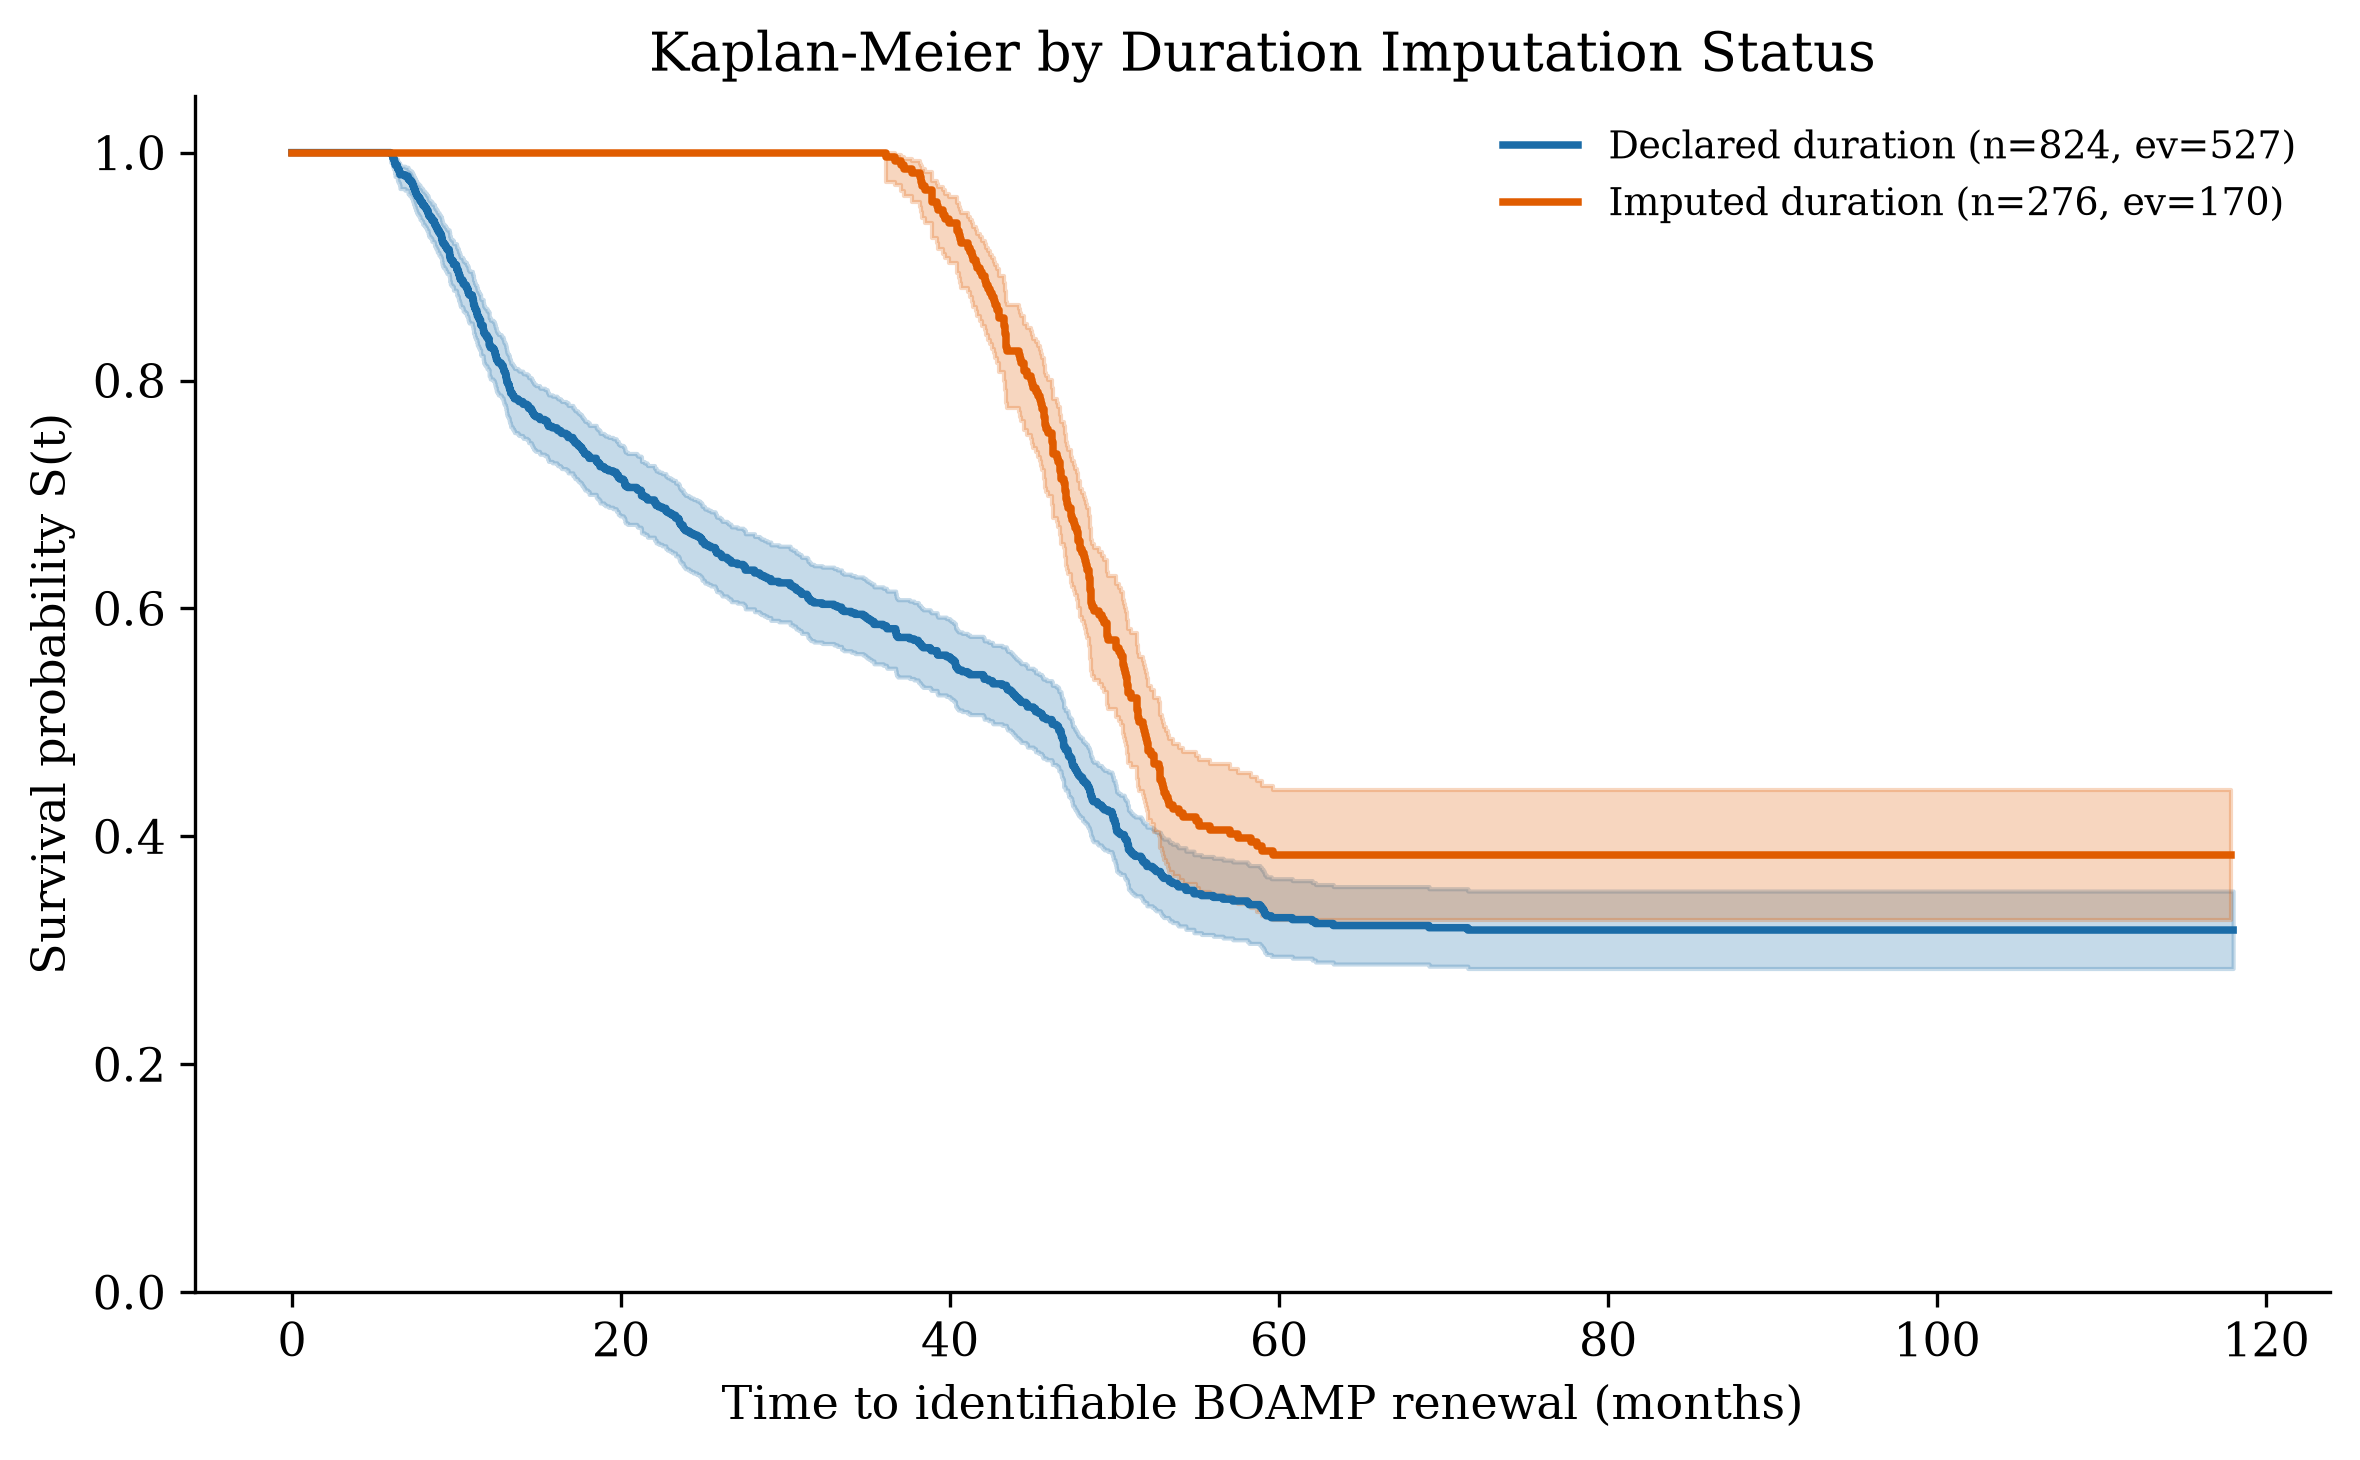
\includegraphics[width=0.88\textwidth]{figures/survival/km_by_imputed}
\caption{Kaplan--Meier survival curves by duration imputation status.
Log-rank test: $\chi^2 = 24.58$, $p \approx 0$, $\mathrm{df} = 1$.
Contracts with imputed durations (48-month default) renew later than
those with observed durations.}
\label{fig:km_imputed}
\end{figure}

\subsection{Log-Rank Test Summary}

Table~\ref{tab:logrank} collects all log-rank test results. Declared duration
group and imputation status are both highly significant. Service category and
procedure type are not significant at the 5\% level.

\begin{table}[H]
\centering
\caption{Log-rank test results for stratified Kaplan--Meier comparisons}
\label{tab:logrank}
\begin{tabular}{@{}P{6.5cm}R{2.4cm}R{1.8cm}R{1.0cm}@{}}
\toprule
Variable & $\chi^2$ statistic & $p$-value & df \\
\midrule
\texttt{declared\_duration\_group} ($\leq 24$, 25--48, $> 48$ mo) & 62.30 & $<0.001$ & 2 \\
\texttt{dur\_was\_imputed} (imputed vs.\ observed) & 24.58 & $<0.001$ & 1 \\
\texttt{category\_label} (5-level ICT category) & 6.23 & 0.182 & 4 \\
\texttt{type\_procedure} (3-level collapsed) & 2.06 & 0.357 & 2 \\
\bottomrule
\end{tabular}
\end{table}

\subsection{Cox Proportional Hazards Model}

\subsubsection*{Univariate Cox Results}

Table~\ref{tab:cox_univariate} reports univariate Cox models for each
covariate. A hazard ratio $> 1$ indicates a higher instantaneous renewal
rate (faster time-to-renewal). Declared duration has the strongest predictive
signal (concordance 0.660), followed by imputation status (0.571).

\begin{table}[H]
\centering
\caption{Univariate Cox proportional hazards results}
\label{tab:cox_univariate}
\small
\begin{tabular}{@{}P{5.0cm}R{1.3cm}R{2.8cm}R{1.8cm}R{2.0cm}@{}}
\toprule
Covariate & HR & 95\% CI & $p$-value & Concordance \\
\midrule
\texttt{declared\_duration\_months}        & 0.985 & [0.981,\ 0.989] & $<0.001$ & 0.660 \\
\texttt{dur\_was\_imputed}                 & 0.652 & [0.548,\ 0.776] & $<0.001$ & 0.571 \\
\texttt{start\_year}                       & 1.167 & [1.119,\ 1.217] & $<0.001$ & 0.591 \\
\midrule
\multicolumn{5}{l}{\textit{--- Category (ref: Cybersecurity) ---}} \\
IT Services \& Consulting                  & 1.152 & [0.980,\ 1.355] & 0.086 & 0.512 \\
Other                                      & 0.846 & [0.704,\ 1.017] & 0.076 & 0.505 \\
Software \& Applications                   & 1.085 & [0.905,\ 1.301] & 0.377 & 0.498 \\
Telecom \& Networks                        & 0.896 & [0.736,\ 1.092] & 0.277 & 0.505 \\
\midrule
\multicolumn{5}{l}{\textit{--- Procedure (ref: N\'egoci\'e) ---}} \\
OUVERT                                     & 1.113 & [0.958,\ 1.293] & 0.162 & 0.526 \\
Other procedure                            & 0.665 & [0.392,\ 1.129] & 0.131 & 0.504 \\
PROCEDURE\_ADAPTE                          & 0.910 & [0.779,\ 1.063] & 0.232 & 0.522 \\
\bottomrule
\end{tabular}
\normalsize
\end{table}

\subsubsection*{Multivariate Cox Model}

Table~\ref{tab:cox_multi} reports the final multivariate Cox model including
all covariates. Two predictors are statistically significant at the 1\% level:
\texttt{declared\_duration\_months} and \texttt{start\_year}. The model is fitted
on the 1,097 contracts (696 events) with complete category and procedure
covariates; three rows are dropped for missing covariate values. The model
concordance (C-index) is \textbf{0.6528}, indicating moderate in-sample ranking
ability beyond a random ranking.

\begin{table}[H]
\centering
\caption{Multivariate Cox proportional hazards model (C-index = 0.6528)}
\label{tab:cox_multi}
\small
\begin{tabular}{@{}P{5.8cm}R{1.2cm}R{3.0cm}R{2.0cm}@{}}
\toprule
Covariate & HR & 95\% CI & $p$-value \\
\midrule
\texttt{declared\_duration\_months}        & 0.990 & [0.986,\ 0.995] & $<0.001$\rlap{$^{***}$} \\
\texttt{start\_year}                       & 1.098 & [1.054,\ 1.143] & $<0.001$\rlap{$^{***}$} \\
\texttt{dur\_was\_imputed}                 & 0.862 & [0.716,\ 1.037] & 0.116 \\
\midrule
\multicolumn{4}{l}{\textit{--- Category (ref: Cybersecurity) ---}} \\
IT Services \& Consulting                  & 1.120 & [0.920,\ 1.363] & 0.258 \\
Software \& Applications                   & 1.175 & [0.947,\ 1.457] & 0.143 \\
Telecom \& Networks                        & 0.919 & [0.736,\ 1.147] & 0.453 \\
Other                                      & 0.870 & [0.705,\ 1.074] & 0.194 \\
\midrule
\multicolumn{4}{l}{\textit{--- Procedure (ref: N\'egoci\'e) ---}} \\
OUVERT                                     & 0.979 & [0.789,\ 1.215] & 0.846 \\
PROCEDURE\_ADAPTE                          & 1.028 & [0.821,\ 1.288] & 0.808 \\
Other procedure                            & 0.662 & [0.403,\ 1.088] & 0.104 \\
\midrule
\multicolumn{4}{l}{\small $^{***}\ p < 0.001$} \\
\bottomrule
\end{tabular}
\normalsize
\end{table}

Figure~\ref{fig:forest} shows the forest plot of hazard ratios with 95\%
confidence intervals for all covariates in the multivariate model.

\begin{figure}[H]
\centering
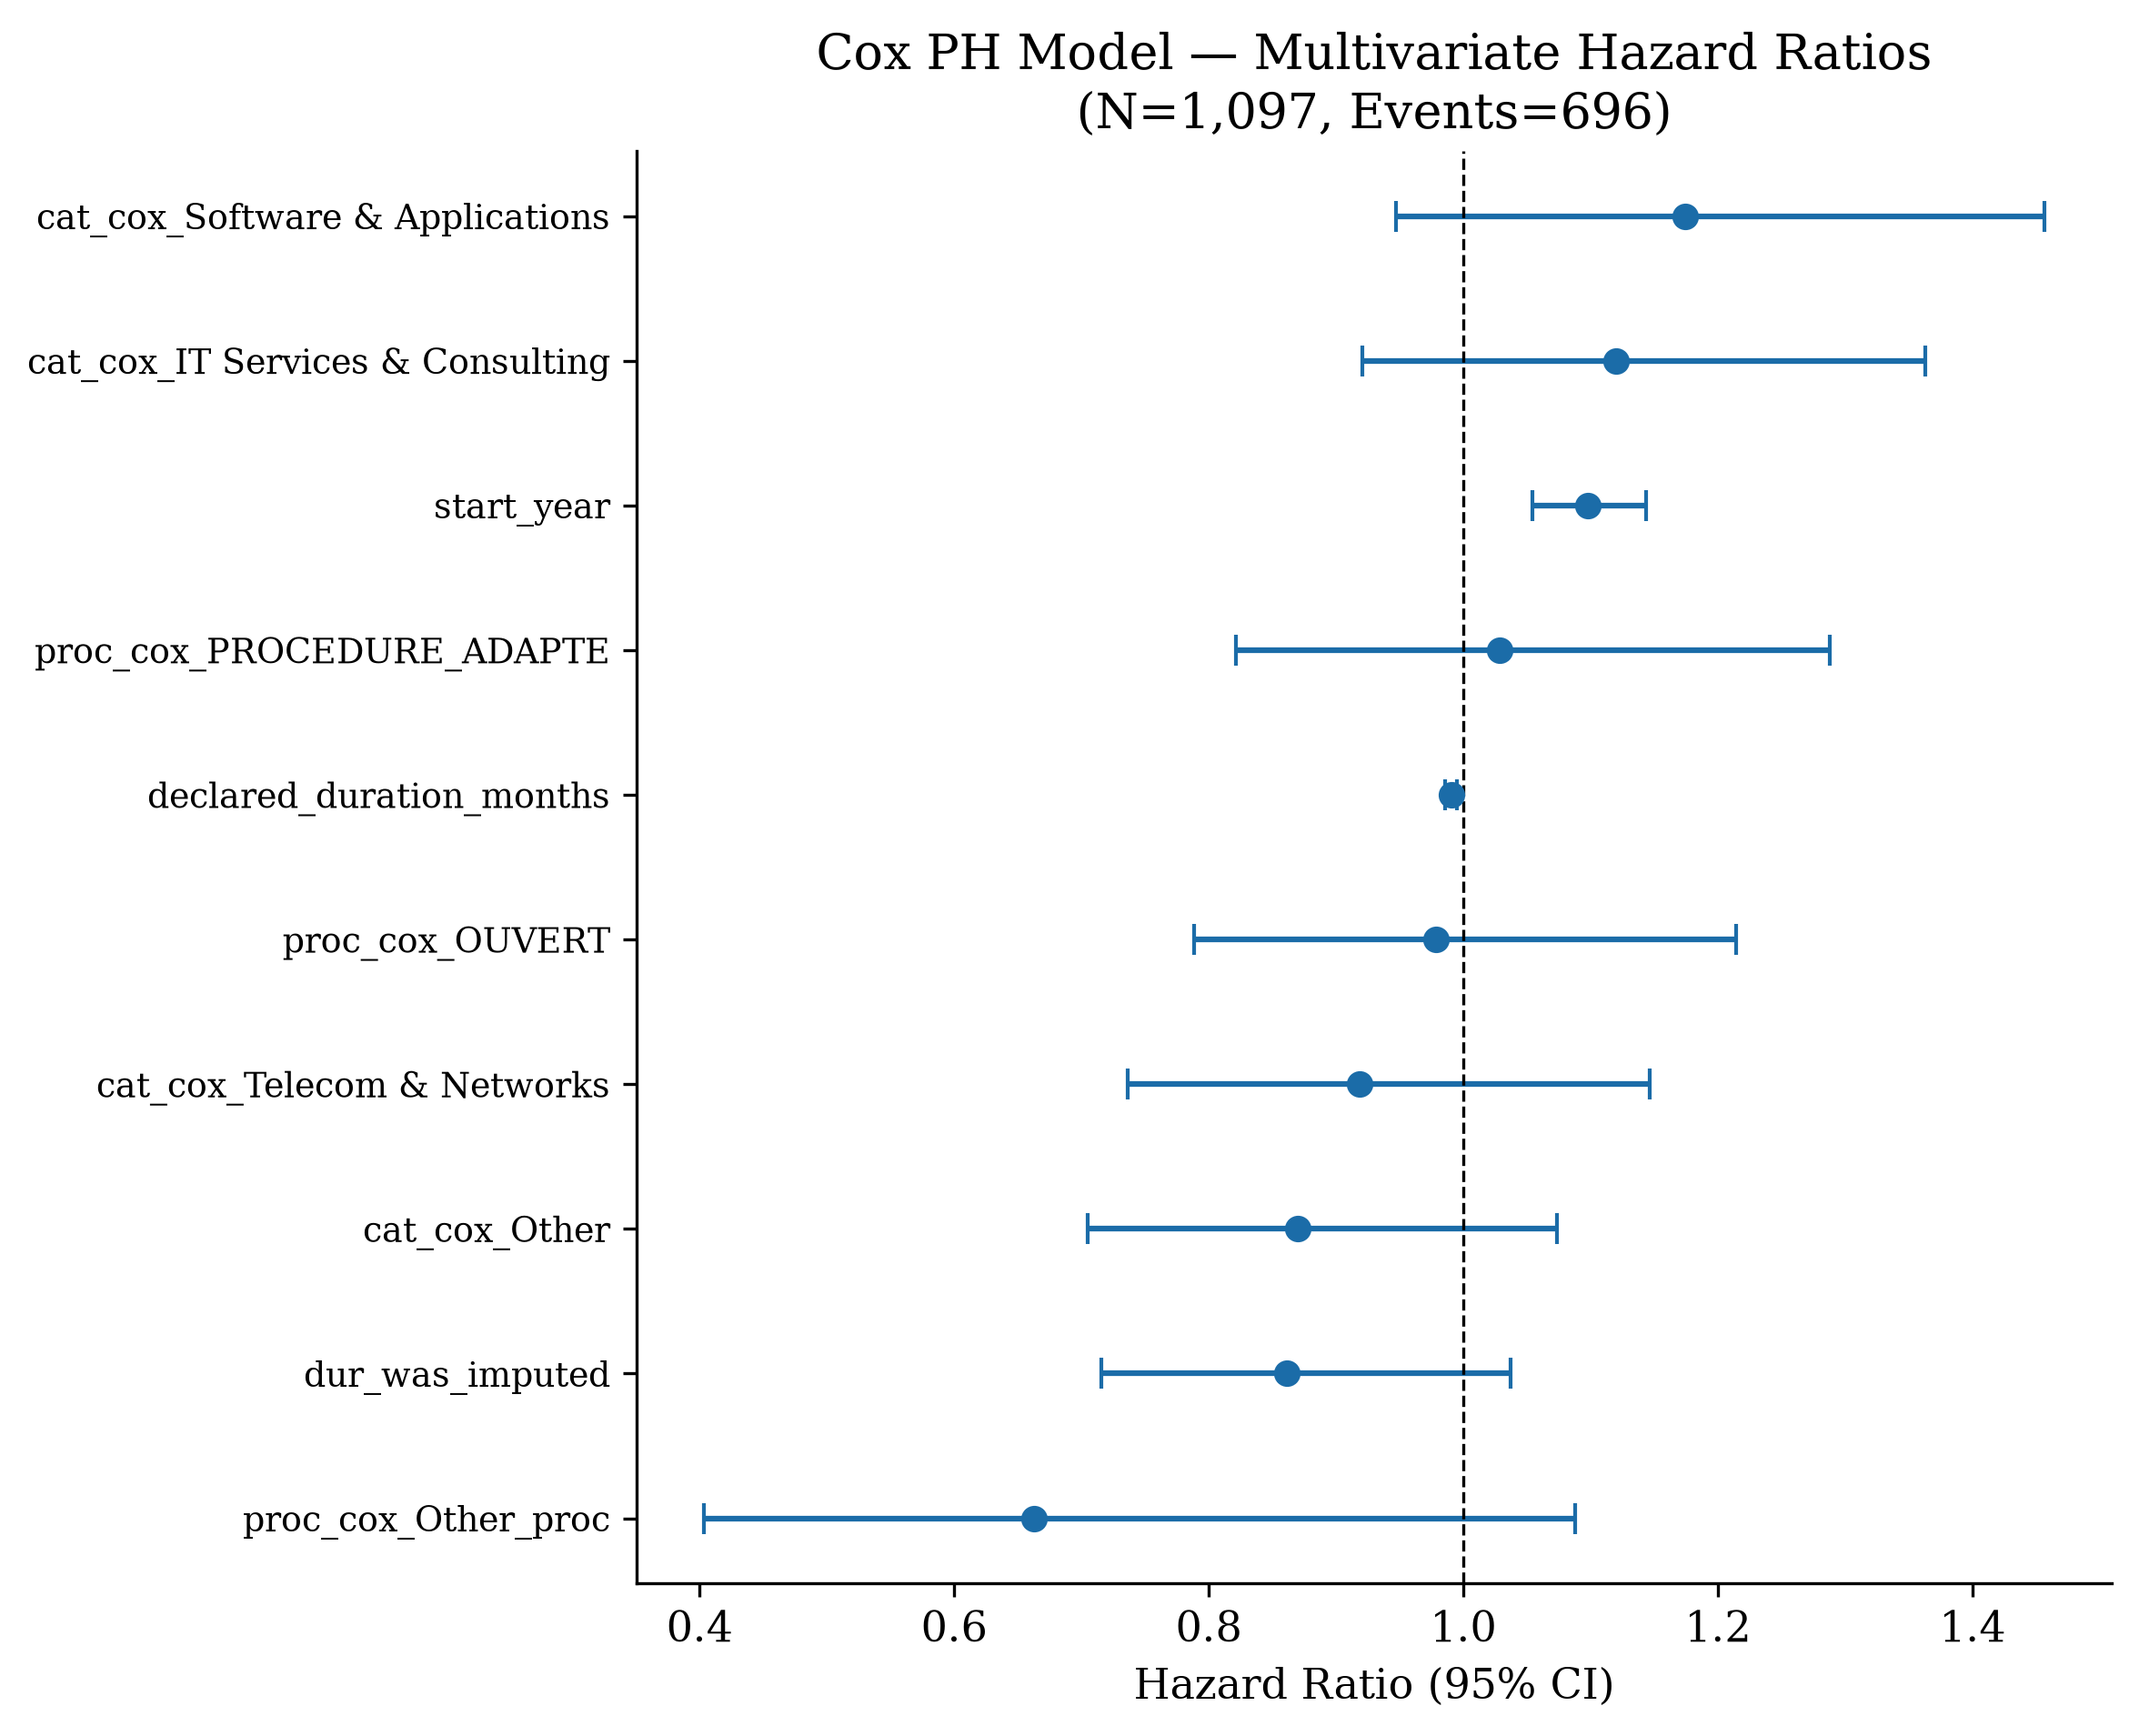
\includegraphics[width=0.90\textwidth]{figures/survival/cox_forest_plot}
\caption{Forest plot of multivariate Cox hazard ratios. Points indicate the
estimated HR; horizontal bars are 95\% confidence intervals. The vertical
dashed line at HR = 1 indicates no effect. Blue/filled markers are
statistically significant at the 5\% level.}
\label{fig:forest}
\end{figure}

\subsubsection*{Proportional Hazards Assumption Check}

The proportional hazards assumption was checked two ways: a formal Schoenfeld
residual test (lifelines \texttt{check\_assumptions}) and a graphical log-log
transformation of the KM survival function. The Schoenfeld test flags a
violation for \texttt{declared\_duration\_months} ($p < 5\times10^{-5}$), the
strongest predictor in the model; the remaining covariates pass. This indicates
a time-varying (non-proportional) effect for declared duration. We interpret
this with caution rather than as invalidating: the Schoenfeld test is highly
sensitive to functional-form misspecification, and the likely cause here is a
mildly non-linear relationship between declared duration and the log-hazard
rather than a true reversal of effect over time. Two facts limit the practical
impact: (i) the parametric AFT models reported below do not rely on the PH
assumption and yield the same directional conclusions; and (ii) the
\texttt{declared\_duration\_months} hazard ratio (HR = 0.990) is consistent in
sign and magnitude across the univariate, multivariate, and sensitivity
specifications. A fully rigorous treatment would stratify on binned declared
duration or add a time interaction; this is flagged as future work.

Figure~\ref{fig:ph_check} shows the $\log(-\log(\hat{S}(t)))$ curves stratified
by imputation status. Approximately parallel lines are consistent with the PH
assumption for that covariate; crossing or diverging lines suggest a violation.

\begin{figure}[H]
\centering
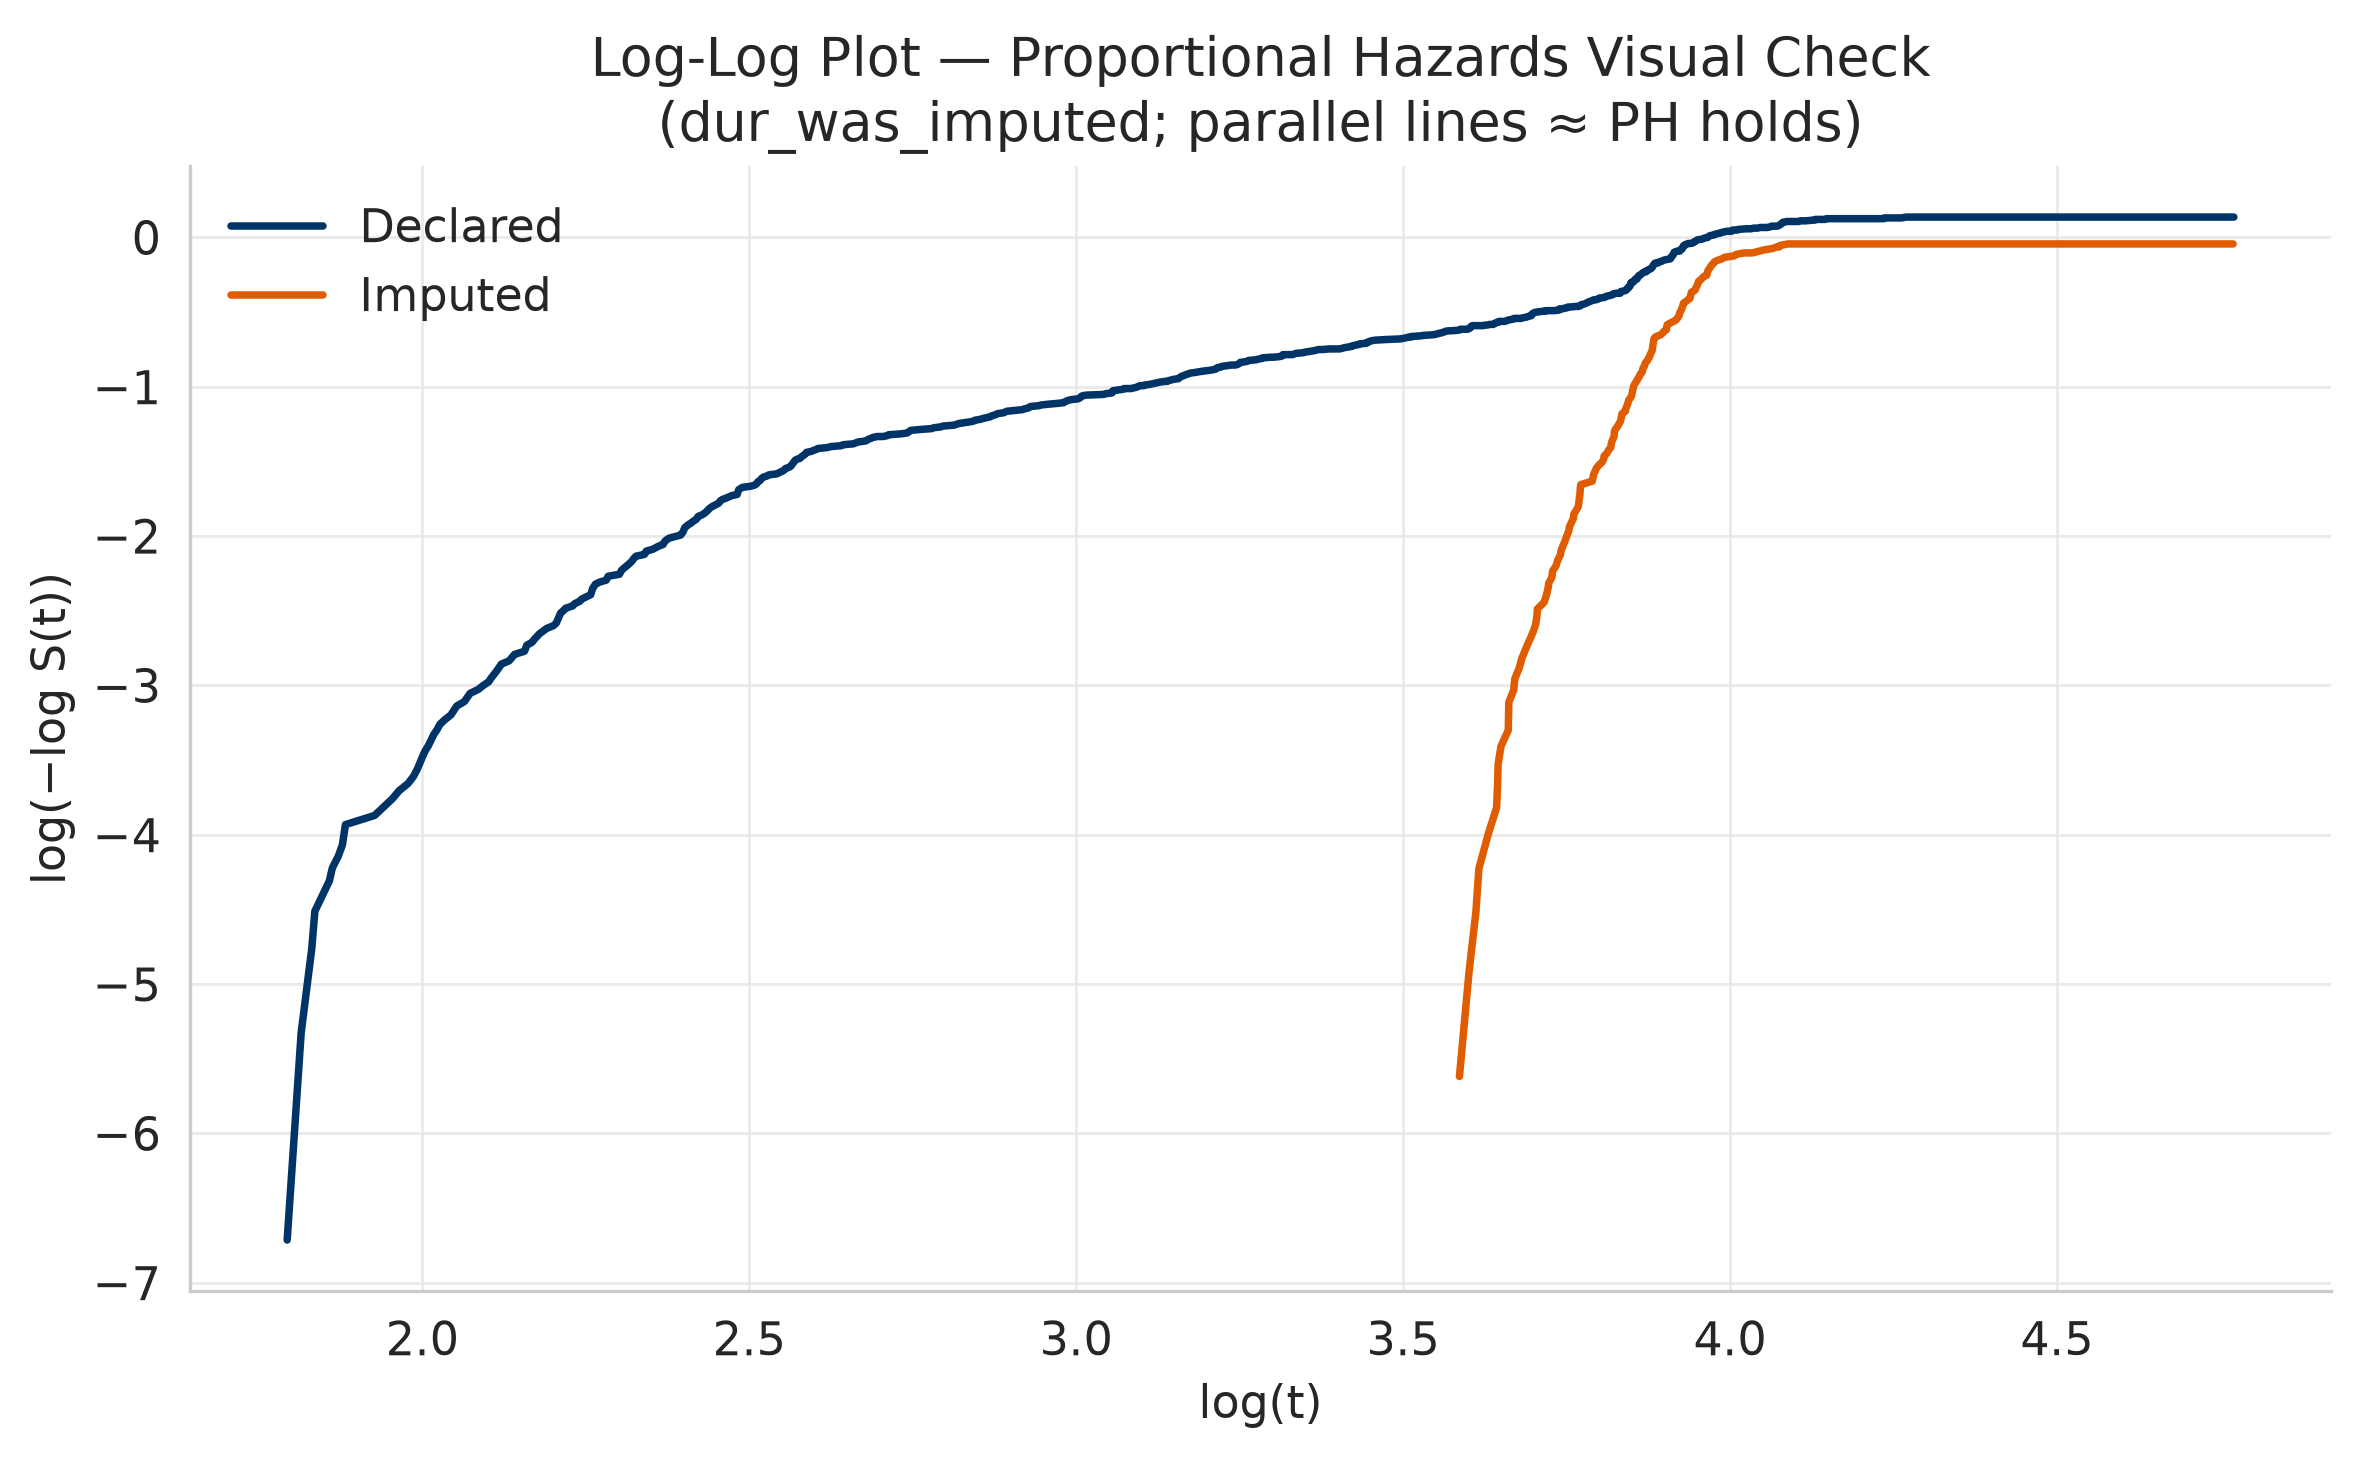
\includegraphics[width=0.88\textwidth]{figures/survival/cox_assumptions}
\caption{Log-log plot for the proportional hazards assumption check,
stratified by duration imputation status (declared vs.\ imputed). The curves
are approximately parallel over the observable time range, consistent with the
PH assumption for this covariate. Note that the formal Schoenfeld test flags
\texttt{declared\_duration\_months} as non-proportional (see text).}
\label{fig:ph_check}
\end{figure}

\subsection{Parametric Survival Models}

Three accelerated failure time (AFT) models were fitted to assess parametric
alternatives to the semi-parametric Cox model. Table~\ref{tab:aft} compares
goodness-of-fit (AIC) and concordance across distributional families.

\begin{table}[H]
\centering
\caption{Parametric AFT model comparison}
\label{tab:aft}
\begin{tabular}{@{}lR{2.4cm}R{2.4cm}@{}}
\toprule
Model & AIC & Concordance \\
\midrule
\textbf{Log-Normal}   & \textbf{7\,119.9} & \textbf{0.671} \\
Log-Logistic          & 7\,196.1          & 0.675 \\
Weibull               & 7\,319.8          & 0.635 \\
\bottomrule
\end{tabular}
\end{table}

The log-normal model achieves the lowest AIC (7\,119.9) and a concordance of
0.671, marginally above the Cox model (0.653). The log-logistic model achieves
the highest concordance (0.675) at the cost of a higher AIC. The Weibull model
performs worst on both metrics. These results suggest that the renewal gap
distribution has a heavier tail than the Weibull's exponential hazard allows,
and that the non-monotone hazard shape of the log-normal/log-logistic models
better captures the data.

Figure~\ref{fig:aft} overlays the three parametric predicted survival curves
against the empirical Kaplan--Meier estimate.

\begin{figure}[H]
\centering
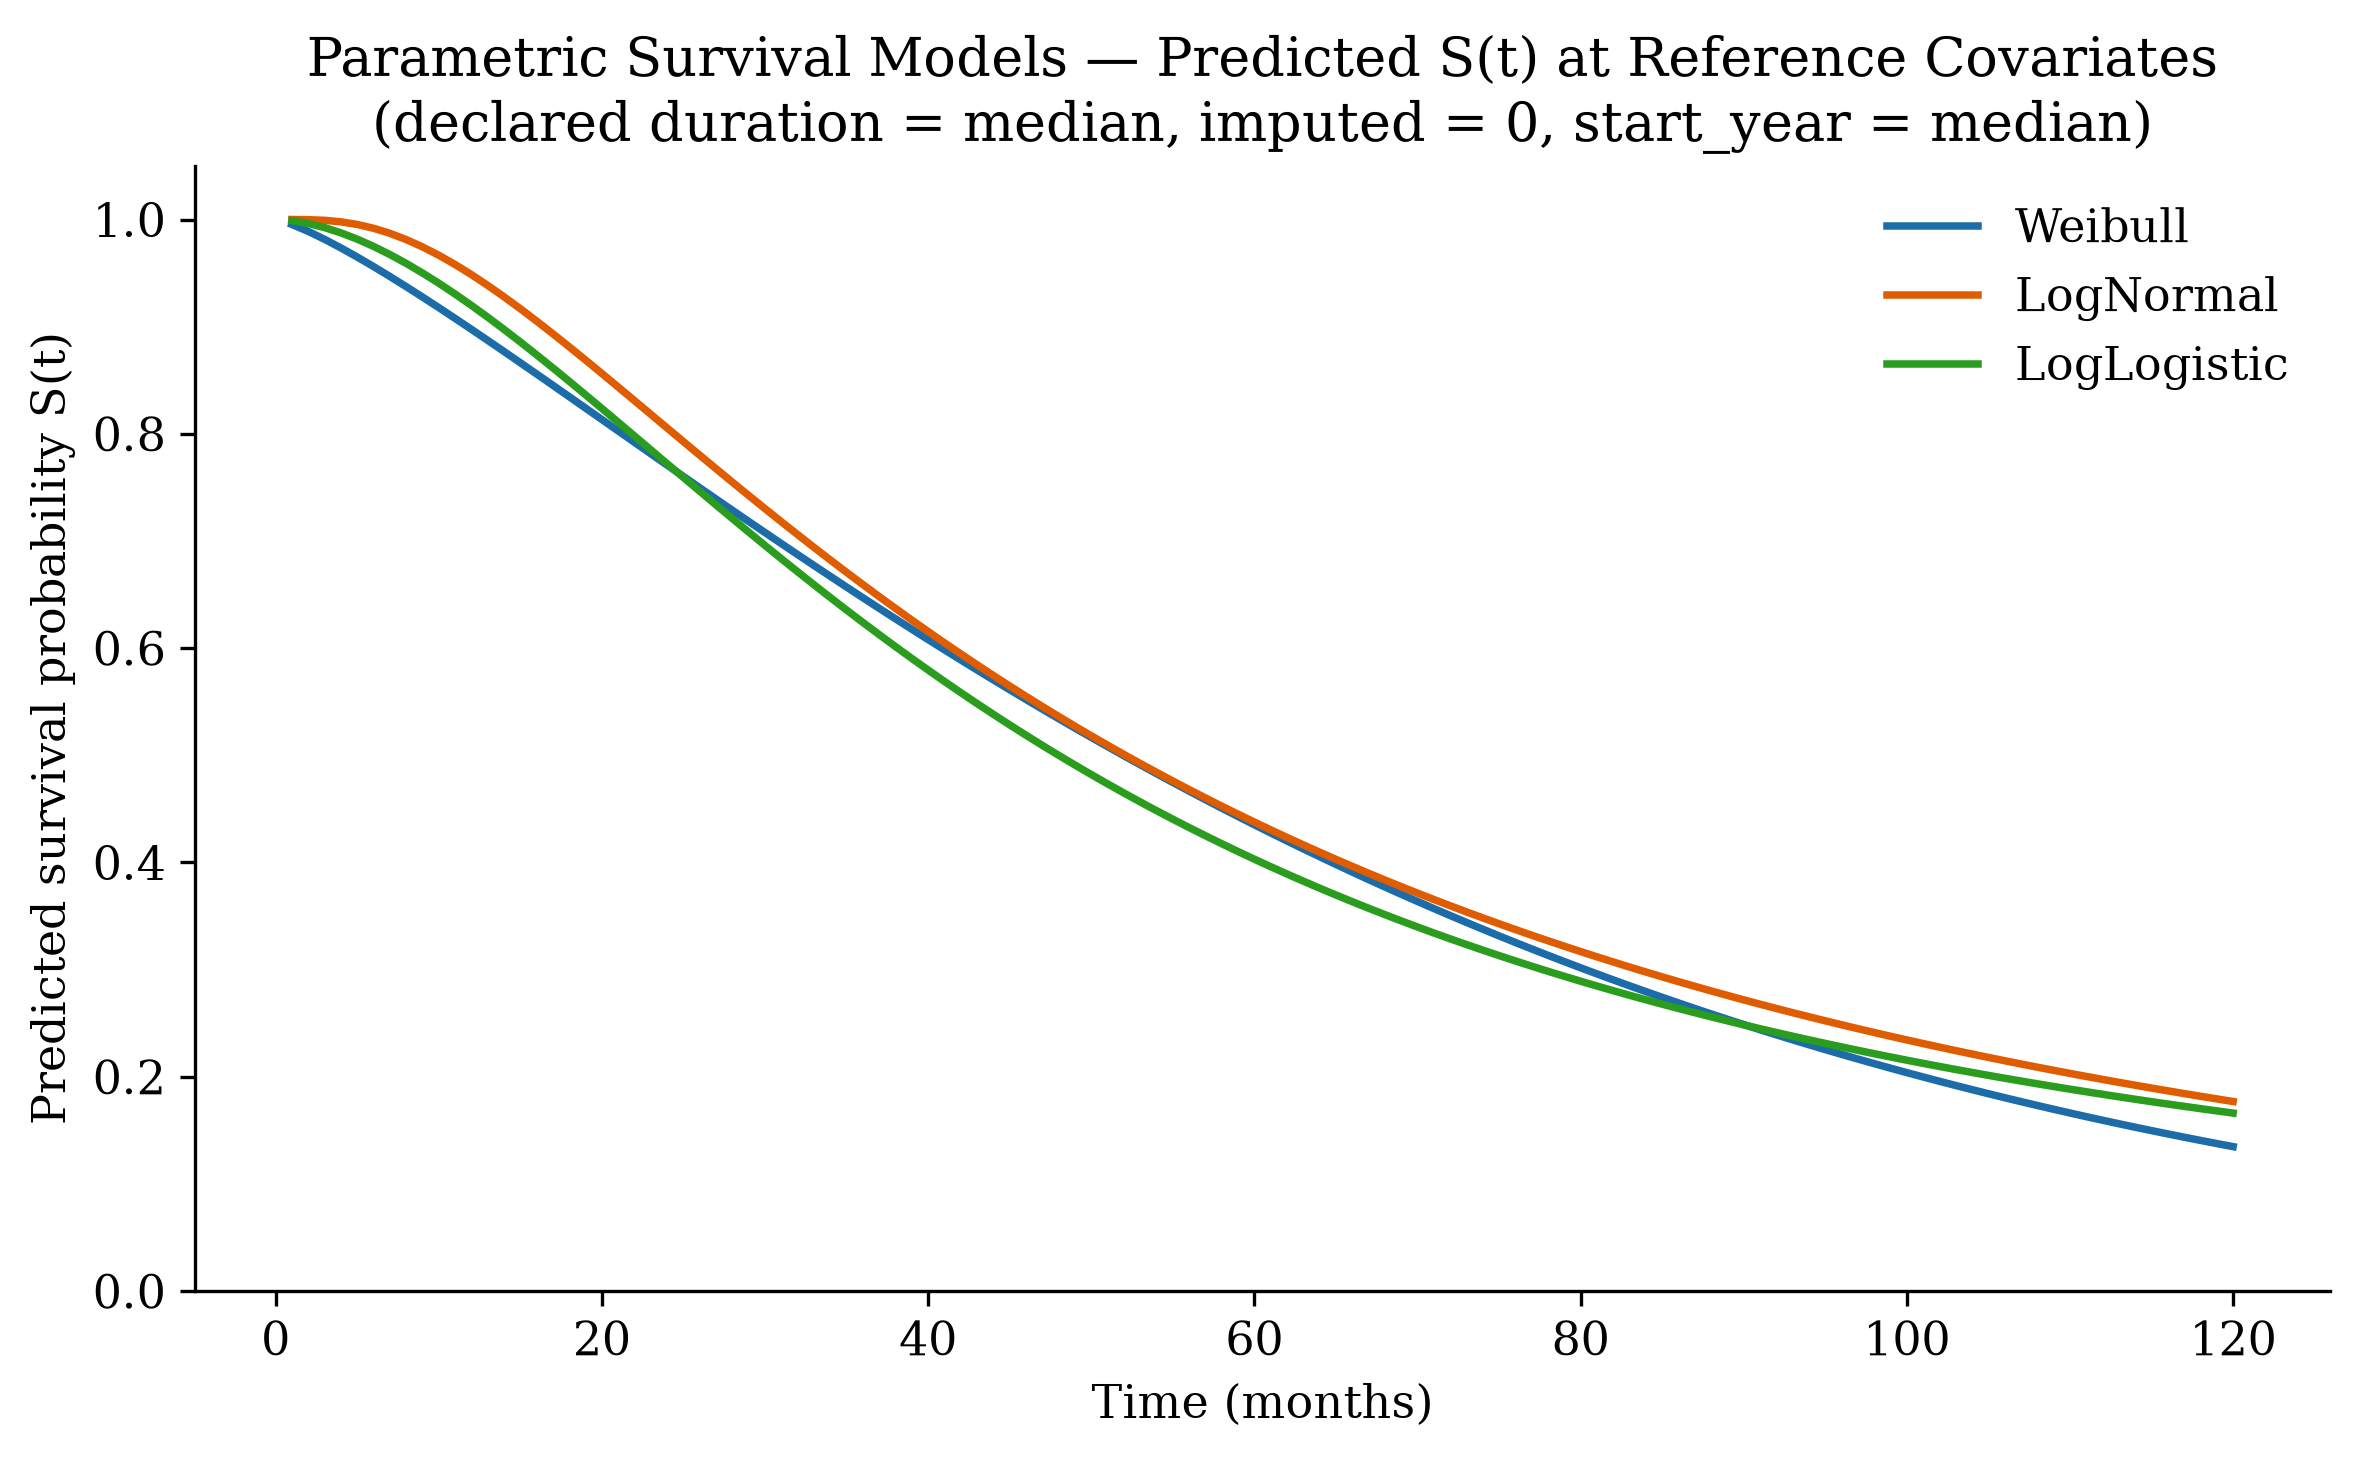
\includegraphics[width=0.90\textwidth]{figures/survival/weibull_survival}
\caption{Parametric survival predictions from the three AFT models (Weibull,
Log-Normal, Log-Logistic) overlaid on the empirical Kaplan--Meier curve.
The log-normal fit is closest to the KM estimate, consistent with its lower AIC.
The Weibull model underestimates survival at early times and overestimates at
late times.}
\label{fig:aft}
\end{figure}

\subsection{Sensitivity Analysis: Model A vs.\ Model B}

Two model configurations were compared to assess the impact of low-confidence
links (Section~\ref{sec:reliability}) on the survival estimates.

\begin{table}[H]
\centering
\caption{Sensitivity analysis: Model A (baseline) vs.\ Model B (conservative)}
\label{tab:sensitivity}
\begin{tabular}{@{}P{6.5cm}R{2.0cm}R{2.0cm}@{}}
\toprule
Metric & Model A & Model B \\
\midrule
Event threshold & composite $\geq 0.20$ & composite $\geq 0.50$ \\
Events & 697 & 553 \\
Censored & 403 & 547 \\
Event rate & 63.4\% & 50.3\% \\
KM median survival & 48.0 mo & 53.0 mo \\
Cox C-index & 0.6528 & 0.6202 \\
\bottomrule
\end{tabular}
\end{table}

\noindent\textbf{Interpretation.} Restricting to high- and medium-confidence
links (Model B) shifts the KM median upward by 5 months, consistent with the
excluded LOW-tier links being concentrated at shorter observed gaps (lower text
similarity often corresponds to borderline temporal matches). The Cox concordance
decreases slightly from 0.653 to 0.620 because the smaller event count reduces
statistical power, not because the conservative definition produces a worse
model. The qualitative conclusions --- declared duration and start year as the
dominant predictors, no significant category or procedure effect --- are stable
across both models.

Figure~\ref{fig:sensitivity} overlays the KM curves from both models.

\begin{figure}[H]
\centering
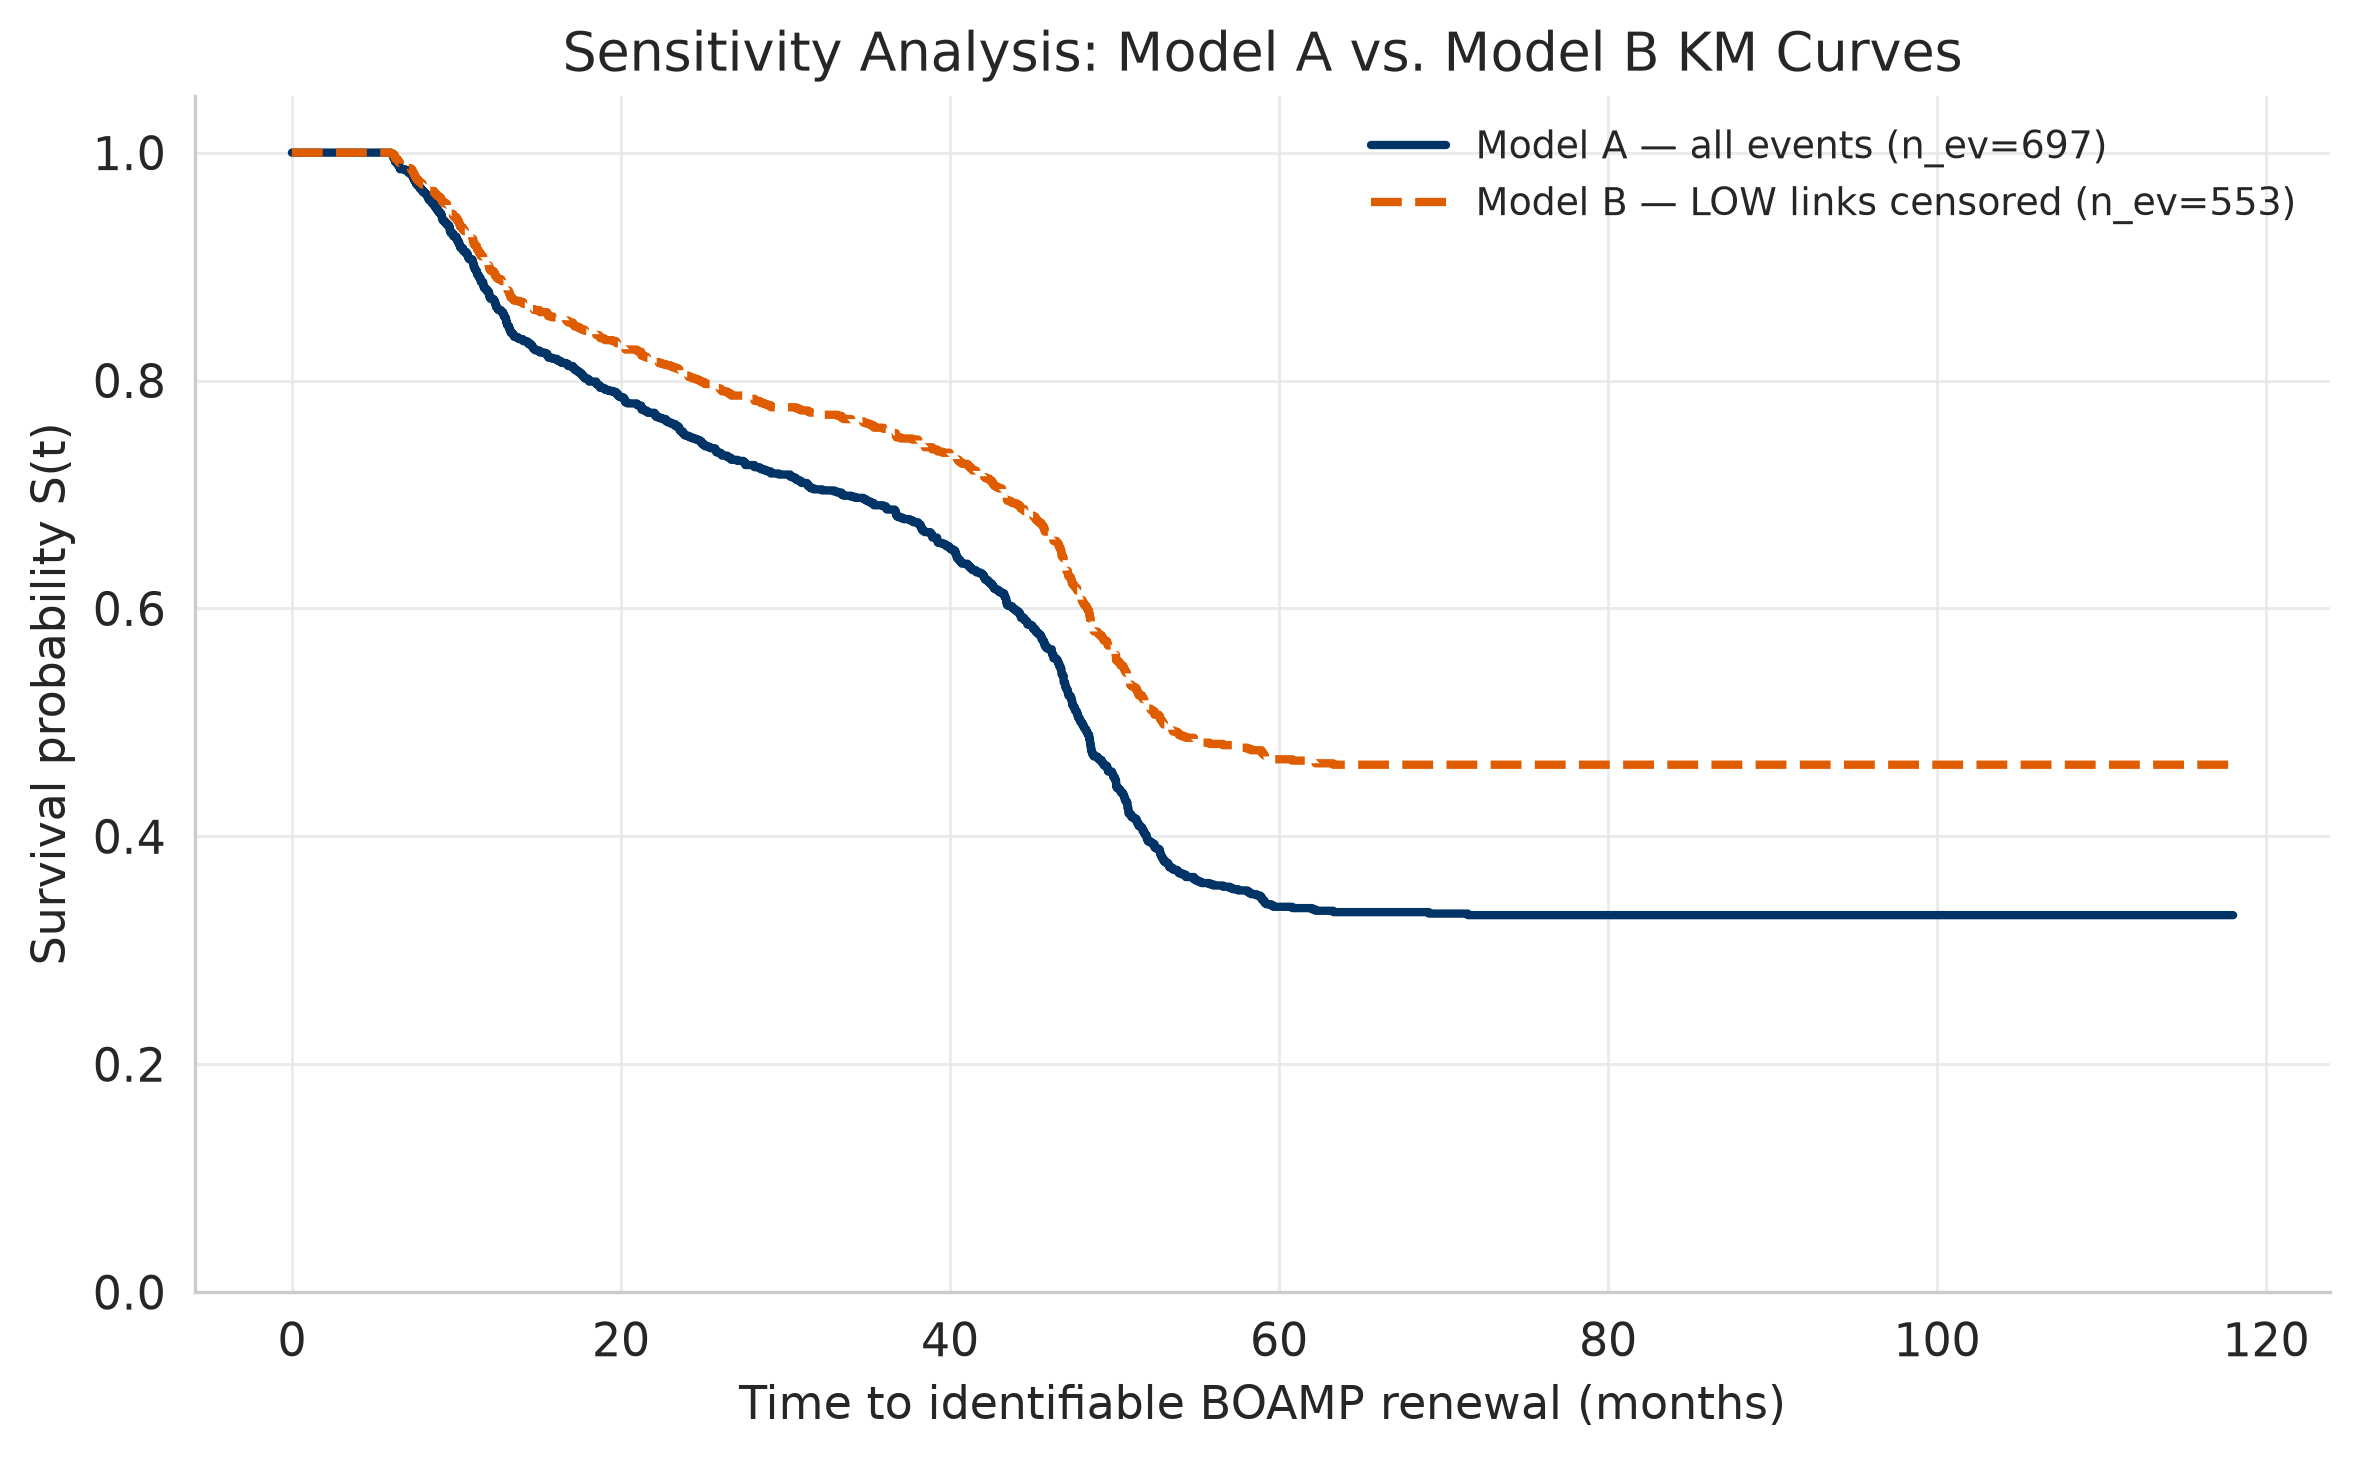
\includegraphics[width=0.88\textwidth]{figures/survival/sensitivity_km_comparison}
\caption{Kaplan--Meier comparison: Model A (all 697 linked contracts, blue) vs.\
Model B (553 high/medium-confidence contracts, orange). The conservative model
produces a higher median estimate (53.0 mo vs.\ 48.0 mo) but the overall curve
shapes and confidence intervals are broadly consistent, confirming that the
LOW-confidence links add noise but do not introduce systematic bias.}
\label{fig:sensitivity}
\end{figure}

\subsection{Summary of Phase 2 Findings}

\begin{enumerate}[leftmargin=*, label=\textbf{F\arabic*.}]

  \item \textbf{Global median renewal time: 48 months.} The KM estimate
        confirms that the 48-month administrative duration is the dominant
        pattern in public procurement renewal. The distribution is right-skewed:
        roughly 25\% of contracts renew within 24 months.

  \item \textbf{Two statistically significant predictors.} In the multivariate
        Cox model, only \texttt{declared\_duration\_months} (HR = 0.990,
        $p < 0.001$) and \texttt{start\_year} (HR = 1.098, $p < 0.001$) are
        significant. Shorter declared durations predict faster renewal.
        The positive \texttt{start\_year} hazard ratio indicates that more
        recent contracts renew faster, possibly reflecting an accelerating
        procurement cycle or left-truncation of older contracts in the study period.

  \item \textbf{No significant category or procedure effect.} None of the
        ICT service categories or procurement procedure types differ
        significantly from their reference in the multivariate model ($p > 0.10$
        for all). Log-rank tests confirm this at the bivariate level.

  \item \textbf{Log-normal AFT model preferred.} Among parametric models, the
        log-normal achieves the best trade-off between fit (AIC = 7\,119.9) and
        concordance (0.671), outperforming the Cox model marginally. The Weibull
        model is the worst fit.

  \item \textbf{Sensitivity check supports qualitative stability.} Restricting to
        high/medium-confidence links (Model B) shifts the median by $+5$ months
        but leaves the covariate effects qualitatively unchanged. The primary
        model (Model A) is retained as the official result.

\end{enumerate}

% =============================================================================
\section{Remaining Next Steps}

Phase 2 is complete. The remaining planned phases are:

\begin{enumerate}
  \item \textbf{Phase 3 --- Validation:} Manual annotation of a stratified sample
        of 50--100 linked pairs to estimate precision. Sensitivity analysis on
        the composite score threshold and temporal window width.
  \item \textbf{Phase 4 --- Optional enrichment:} Revisit DECP integration only
        after the BOAMP-only model is stabilized and a defensible cross-source
        linkage strategy is defined.
  \item \textbf{Phase 5 --- Production pipeline:} Operationalise as a monthly
        batch job on new BOAMP notices.
\end{enumerate}

\end{document}
